%                                     MMMMMMMMM
%
%  MMA    MM   MMMMMM  MMMMMMM   MM    MMMMMMMM   MMA   MM  MMMMMMM MMMMMMM
%  MMMA AMMM   MM        MM     MMMM              MMMM  MM  MM        MM
%  MM MMM MM   MMMMMM    MM    IM  MI   MMMMMMM   MM MMxMM  MMMMMM    MM
%  MM  M  MM   MM        MM   .MMMMMM.            MM  MMMM  MM        MM
%  MM     MM   MMMMMM    MM   MM    MM            MM   MMM  MMMMMMM   MM
%
%
%            - META-NET Language White Paper | Croatian content -
% 
% ----------------------------------------------------------------------------

\begin{document}

\maketitle

% --------------------------------------------------------------------------
\bsection*{Predgovor --- Preface}

\null
\pagestyle{empty} 

\pagenumbering{Roman} 
\setcounter{page}{3}
\pagestyle{scrheadings}

\begin{Parallel}[c]{78mm}{78mm}
\ParallelLText{\selectlanguage{croatian}
Ova bijela knjiga dio je niza koji promiče jezične tehnologije i njihove mogućnosti. Namijenjena je novinarima, političarima, jezičnim zajednicama, učiteljima, predavačima i ostalima. Dostupnost i uporaba jezičnih tehnologija u Europi različita je od jezika do jezika. Susljedno, različite su i aktivnosti potrebne za daljnju potporu istraživanjima i razvoju jezičnih tehnologija od jezika do jezika. Potrebne akcije ovise o mnogo čimbenika kao što su složenost pojedinoga jezika i veličina dotične jezične zajednice. 

Mreža izvrsnosti META-NET, koju podupire Europska komisija, provela je analizu trenutačno raspoloživih jezičnih resursa i tehnologija u ovome nizu bijelih knjiga (s.~\pageref{whitepaperseries}). Ta je analiza usredotočena ponajprije na 23 službena jezike Europske unije, ali i na ostale važne nacionalne i regionalne jezike u Europi. Rezultati ove analise ukazuju na nesrazmjerne nedostatke u tehnološkoj potpori i značajne istraživačke nedostatke za svaki od promatranih jezika. Predstavljena podrobna stručna analiza i procjena trenutačne situacije pomoći će u učinkovitosti dodatnih istraživanja u tome smjeru.

Od mjeseca studenoga 2011. META-NET se sastoji od 54 istraživačka središta iz 33 europske zemlje (s.~\pageref{metanetmembers}). META-NET surađuje s ključnim dionicima iz gospodarstva (tvrtke koje izgrađuju programsku podršku, tehnološki isporučitelji, korisnici), vladinim agencijama, istraživačkim organizacijama, nevladinim organizacijama, jezičnih zajednicama i europskim sveučilištima. Zajedno s njima META-NET stvara zajedničku tehnološku viziju i strateški plan za višejezičnu Europu 2020.
}

\ParallelRText{\selectlanguage{english}
This white paper is part of a series that promotes knowledge about language technology and its potential. It addresses journalists, politicians, language communities, educators and others. The availability and use of language technology in Europe varies between languages. Consequently, the actions that are required to further support research and development of language technologies also differs. The required actions depend on many factors, such as the complexity of a given language and the size of its community.

META-NET, a Network of Excellence funded by the European Commission, has conducted an  analysis of current language resources and technologies in this white paper series (p.~\pageref{whitepaperseries}). The analysis focused on the 23 official European languages as well as other important national and regional languages in Europe. The results of this analysis suggest that there are tremendous deficits in technology support and significant research gaps for each language. The given detailed expert analysis and assessment of the current situation will help maximise the impact of additional research.

As of November 2011, META-NET consists of 54 research centres from 33 European countries (p.~\pageref{metanetmembers}). META-NET is working with stakeholders from economy (software companies, technology providers, users), government agencies, research organisations, non-governmental organisations, language communities and European universities. Together with these communities, META-NET is creating a common technology vision and strategic research agenda for multilingual Europe 2020.} 
\ParallelPar
\end{Parallel}

\makefundingnotice

% --------------------------------------------------------------------------

\cleardoublepage

\bsection*{Sadržaj --- Contents}

\renewcommand\contentsname{}
\tableofcontents

\addtocontents{toc}{\protect\thispagestyle{empty}\protect}
\addtocontents{toc}{{\Large\textsf{\centerline{HRVATSKI JEZIK U DIGITALNOM DOBU}}\par}}

% --------------------------------------------------------------------------

\cleardoublepage

\setcounter{page}{1}
\pagenumbering{arabic} 
\pagestyle{scrheadings}

%\ssection[Sažetak]{Sažetak}

\selectlanguage{croatian}

\ssection[Sažetak]{Sažetak}

\selectlanguage{croatian}

\begin{multicols}{2}
Informacijske tehnologije mijenjaju naš svakodnevni život. Uobičajeno se služimo računalima za pisanje, uređivanje, računanje, pretragu obavijesti i sve više za čitanje, slušanje glazbe, pregledavanje fotografija i gledanje filmova. U svojim džepovima nosimo mala računala koja koristimo za obavljanje telefonskih poziva, pisanje e-pošte, prikupljanje obavijesti i za zabavu gdje god se nalazili. Kako ta masovna digitalizacija obavijesti, znanja i svakodnevnih komunikacija utječe na naš jezik? Hoće li se naš jezik promijeniti ili čak nestati? Kakve su mogućnosti hrvatskoga jezika za preživljavanje?

Mnogi od šest tisuća jezika na svijetu ne će preživjeti u globaliziranom digitalnom informacijskom društvu. Procjenjuje se kako je barem dvije tisuće jezika osuđeno na izumiranje u sljedećem desetljeću. Preostali će nastaviti igrati ulogu u privatnome krugu obitelji ili susjedstva, ali ne nužno i na razini općega poslovanja ili na akademskoj razini. Status jezika ne ovisi samo o broju njegovih govornika ili broju knjiga, filmova i TV-postaja koje se njime služe, nego i o prisutnosti toga jezika u digitalnome informacijskome prostoru i u adekvatnoj programskoj podršci.

Ova bijela knjiga o hrvatskome jeziku pokazuje kako u Hrvatskoj postoji temeljno okružje za istraživanje jezičnih tehnologija, međutim to nije rezultiralo i razvojem jezične industrije. Unatoč tome što su za hrvatski izrađeni neki jezični resursi i tehnologije, znatno ih je manje nego za druge slavenske jezike, npr. češki, a još ih je manje razvijeno u usporedbi s većim europskim jezicima kao što su engleski, njemački ili francuski. Prema procjenama podrobnije iznesenim u ovome izvješću, potrebno je poduzeti niz ciljanih mjera kako bi se hrvatski jezični resursi i alati doveli na istu razinu razvijenosti glede njihove kakvoće i količine, kakva je razina već dosegnuta za druge europske jezike.

Vizija META-NET-a su visokokvalitetne jezične tehnologije za sve jezike koje podupiru političko i gospodarsko jedinstvo kroz kulturnu raznolikost. Ove će tehnologije pomoći u uklanjanju prepreka i u izgradnji mostova između jezika u Europi. To, međutim, traži od svih dionika ovoga procesa – politike, istraživanja, gospodarstva i društva u cjelini – objedinjavanje svojih napora u budućnosti.

Ovaj niz bijelih knjiga nadopunjuje ostale strateške aktivnosti koje poduzima META-NET. Najnovije obavijesti, kao što su trenutačna inačica vizije META-NET-a \cite{str1} ili Strateški istraživački plan (SIP) može se pronaći na META-NET-ovim mrežnim stranicama: http://www.meta-net.eu.

\end{multicols}

\clearpage

% --------------------------------------------------------------------------

\ssection[Jezici u opasnosti: izazov za jezične tehnologije]{Jezici u opasnosti: izazov za jezične tehnologije}

\begin{multicols}{2}

U ovome trenutku svjedočimo digitalnoj revoluciji koja korjenito utječe na našu komunikaciju i naše društvo. Najnoviji razvoj digitalnih i mrežnih komunikacijskih tehnologija ponekad se uspoređuju s Gutenbergovim izumom tiska pomičnim slovima. Što nam ta analogija može reći o budućnosti europskoga informacijskoga društva i o našim vlastitim jezicima?

\boxtext{Digitalna revolucija usporediva je s Gutenbergovim izumom tiska pomičnim slovima.}

Nakon Gutenbergova izuma pravi su proboji u komunikaciji i razmjeni znanja postignuti pothvatima kao što je Lutherov prijevod Biblije na narodni jezik (ili u hrvatskome slučaju, glagoljički prvotisak Misala iz 1483. kao prve tiskanje knjige na hrvatskome jeziku). U nadolazećim stoljećima razvijeni su razni kulturni postupci koji su omogućili  obradbu jezika i razmjenu znanja:

\begin{itemize}
\item pravopisno i gramatičko normiranje većih jezika omogućilo je brzu razmjenu novih znanstvenih ideja;
\item uspostavljanje službenih jezika omogućilo je građanima komu-ni¬kaciju unutar određenih (često političkih) granica;
\item poučavanje jezika i prevođenje omogućilo je razmjenu preko jezičnih granica;
\item stvaranje uredničkih i bibliografskih normi osiguralo je kakvoću tiskovina;
\item stvaranjem različitih medija kao što su knjige, novine, radio, televizija i drugi, zadovoljavaju se komunikacijske potrebe pučanstva.
\end{itemize}

U zadnjih je dvadeset godina informacijska tehnologija omogućila olakšavanje i automatizaciju mnogih procesa:

\begin{itemize}
\item računalna priprema za tisak zamijenila je tipkanje i grafički slog;
\item Microsoft PowerPoint zamijenio je projiciranje s prozirnica;
\item e-pošta omogućuje odašiljanje i primanje dokumenata brže od telefaks uređaja;
\item Skype nudi jeftine internetske telefonske pozive i održavanje virtualnih sastanaka;
\item zajednički formati zapisa zvučnih i vizualnih podataka omogućuju jednostavnu razmjenu multimedijskih sadržaja;
\item tražilice omogućuju pristup www-stranicama na temelju pretrage uporabom ključnih riječi;
\item mrežne usluge poput Google prevoditelja nude brze, ali zato približne prijevode;
\item društvene mreže kao što su Facebook, Twitter i Google+ pospješuju komunikaciju, omogućuju suradnju i dijeljenje obavijesti.
\end{itemize}

Premda su takve aplikacije i usluge višestruko korisne, ipak još ne mogu podupirati u cijelosti održivo, višejezično europsko društvo u kojem informacije i robe mogu slobodno kolati.

\subsection{Jezične granice koče europsko informacijsko društvo}
  
Ne možemo točno predvidjeti kako će izgledati buduće informacijsko društvo, ali s velikom se vjerojatnošću može očekivati kako će revolucija u komunikacijskim tehnologijama na nove načine zbližiti ljude koji govore različite jezike. To će kod pojedinaca rezultirati potrebom za učenjem novih jezika, a kod razvijatelja aplikacija potrebom za stvaranjem novih tehnoloških aplikacija, ne bi li se osiguralo uzajamno razumijevanje i omogućio pristup razmjenjivome znanju. U globalnome gospodarskom i informacijskome prostoru raste interakcija između različitih jezika, govornika i sadržaja koja se odvija zahvaljujući novim vrstama medija. Trenutačna popularnost društvenih mreža (kao što su Wikipedia, Facebook, Twitter, YouTube i od nedavno Google+) predstavlja samo vršak ledene sante. 

\boxtext{Globalizacija gospodarstva i informacijskoga prostora suočava nas sa sve više različitih\\ jezika, govornika i sadržaja.}

Danas bez ikakvih prepreka možemo u nekoliko sekunda na drugu stranu svijeta prebaciti gigabajte teksta prije nego što uopće shvatimo kako je on na jeziku koji uopće ne razumijemo. Prema nedavnome izvješću Europske komisije, 57\% internetskih korisnika u Europi putem mreže kupuje robu i usluge na jeziku koji nije njihov vlastiti. Engleski je najčešći strani jezik, a slijede ga francuski, njemački i španjolski. 55\% korisnika čita sadržaje na stranome jeziku dok ih se samo 35\% koristi stranim jezikom za pisanje poruka e-pošte ili ostavljanje komentara na www-u \cite{str2}. Prije nekoliko godina engleski je možda bio \emph{lingua franca} www-a jer je većina sadržaja na www-u tada bila na engleskome, međutim, danas su se prilike u mnogome promijenile. Moglo bi se reći kako je količina sadržaja na drugim jezicima (osobito azijskim i na arapskome) upravo eksplodirala. Iznenađujuće je kako ovaj sveprisutni digitalni jaz prouzrokovan jezičnim preprekama još uvijek nije privukao dovoljno pozornosti u javnim raspravama; pa ipak, upravo nas on navodi na goruće pitanje: „Koji će europski jezici napredovati i održati se u umreženome informacijskome društvu i društvu znanja, a koji će biti osuđeni na izumiranje?“

\subsection{Opasnost za naše jezike}

Dok je otkriće tiska neizmjerno pridonijelo razmjeni obavijesti u Europi, ono je istodobno dovelo do izumiranja mnogih europskih jezika. Kako se na regionalnim i manjinskim jezicima tiskalo rijetko, mnogi su jezici, npr. cornwallski ili dalmatski, bili ograničeni samo na govorni oblik komunikacije što je ograničilo doseg njihove uporabe. Hoće li Internet imati isti utjecaj na naše današnje jezike? Osamdesetak europskih jezika najbogatiji je i najvažnijih dio njezina kulturnoga nasljeđa i neizostavni dio jedinstvenoga društvenoga modela \cite{str3}. Dok će široko korišteni jezici kao engleski ili španjolski zacijelo održati svoju prisutnost na rastućem tržištu digitalnoga društva, mnogi bi europski jezici mogli biti isključeni iz digitalnih komunikacijskih kanala i postati nevažni za takvo umreženo društvo. Time bi se s jedne strane oslabio globalni položaj Europe, a s druge strane, takav bi razvoj bio u suprotnosti sa strateškim ciljem osiguravanja jednakoga sudjelovanja svakoga građanina EU bez obzira na njegov jezik.

Prema izvješću UNESCO-a o višejezičnosti jezici su ključni medij za ostvarivanje temeljnih ljudskih prava kao što su iskazivanje političkoga stava, obrazovanje i sudjelovanje u društvu \cite{str4}. 

\boxtext{Znatna raznolikost jezika u Europi jedno\\ je od najvažnijih kulturnih dobara i bitan\\ je dio europskoga uspjeha.}

\subsection{Jezične su tehnologije ključne potporne tehnologije}

U prethodnim razdobljima ulaganje u jezike usredotočivalo se na učenje jezika i prevođenje. Na primjer, prema nekim procjenama europsko tržište prevođenja, tumačenja, lokalizacije programske podrške i prevođenja www-stranica vrijedilo je 8,4 milijarde eura, a očekivao se njegov rast od 10\% godišnje \cite{str5}. No čak i uz takve prognoze rasta postojeći kapaciteti nisu dovoljni za zadovoljenje potreba niti sadašnjih, a kamoli budućih potreba. Najuvjerljivije rješenje koje bi osiguralo širinu i dubinu uporabe jezika u sutrašnjoj Europi jest uporaba odgovarajućih tehnologija, upravo kao što rabimo razne tehnologije pri rješavanju npr. svojih transportnih ili energetskih potreba.

Jezične tehnologije usmjerene na sve vrste pisanoga ili govorenoga teksta, pomažu ljudima u suradnji, obavljanju poslova, razmjeni znanja i sudjelovanju u društvenim i političkim raspravama neovisno o stupnju usvojenih jezičnih ili računalnih vještina. One već često djeluju skrivene unutar složenih računalnih sustava koji nam pomažu kad:

\begin{itemize}
\item tražimo obavijesti korištenjem internetskih tražilica;
\item provjeravamo pravopis ili gramatiku u obradniku teksta;
\item gledamo preporuke za proizvode u on-line dućanima;
\item slušamo glasovne upute navigacijskoga sustava;
\item prevodimo www-stranice uporabom usluge on-line prevođenja.
\end{itemize}

Jezične tehnologije, o kojima se podrobnije govori u ovoj bijeloj knjizi, čine srž budućih inovativnih aplikacija. Jezične su tehnologije uobičajena potporna tehnologija unutar veće aplikacije kao što su navigacijski sustav ili tražilica. Ove bijele knjige prikazuju stanje osnovnih postignuća u jezičnim tehnologijama za svaki pojedini jezik.

\boxtext{Svi će europski jezici trebati jezične\\ tehnologije koje će biti dostupne i prihvatljive.}

Jezične se tehnologije sastoje od niza osnovih aplikacija koje omogućuju uporabu i obradbu jezika i govora unutar složenijih aplikacijskih sustava. Svrha je ovih META-NET-ovih bijelih knjiga prikazati koliko su te osnovne potporne jezične tehnologije razvijene za svaki od europskih jezika. Europa treba robusne i dostupne jezične tehnologije za sve europske jezike. Kako bi održala svoj položaj globalnoga predvonika u inovacijama, Europa treba jezične tehnologije prilagođene svakome od svojih jezika, a one moraju biti robusne i dostupne ne bi li se što lakše integrirale u šire aplikacijsko okružje. Bez jezičnih tehnologija uskoro više ne ćemo moći postići stvarno interaktivno, multimedijsko i višejezično korisničko iskustvo.

\subsection{Mogućnosti jezičnih tehnologija}

U svijetu tiska tehnološki je proboj predstavljalo brzo umnožavanje slike teksta uporabom tiskarskoga stroja pomičnim slovima. Međutim, istodbno je ljudima prepušten težak posao traženja, pristupa, prevođenja i sažimanja znanja širenoga i prenošenoga tako umnoženim tekstovima. Morali smo čekati do Edisona koji je otkrio kako zabilježiti govor, ali ponovno je njegova tehnologija stvarala analogne preslike.

Jezične nam tehnologije danas omogućuju pojednostavnjivanje i automatizaciju postupaka kao što su strojno prevođenje, stvaranje sadržaja, i upravljanje znanjem na svim europskim jezicima. Jezične tehnologije također stoje u pozadini intuitivnih govornih sučelja za kućansku elektroniku, strojeve, vozila, računala i robote. Premda već postoje mnogi prototipovi, komercijalne i industrijske primjene su još uvijek u ranim stupnjevima razvoja. Međutim, neka su nedavna postignuća u istraživanjima i razvoju otvorila jedinstvene mogućnosti. Na primjer, strojnim prevođenjem već se mogu dobiti prijevodi prihvatljive točnosti unutar posebnih područja, dok istodobno neke eksperimentalne aplikacije već omogućuju dohvat višejezičnih obavijesti i upravljanje znanjem, kao i proizvodnju sadržaja istodobno na mnogim europskim jezicima.

Kao što je to bio slučaj i s mnogim drugim tehnologijama, prve su jezične aplikacije, kao što su govorna korisnička sučelja i razgovorni sustavi, ponajprije razvijene u visokospecijaliziranim područjima uporabe, ali nerijetko uz ograničenu kakvoću. Pa ipak i za takve aplikacije postoje ogromne tržišne mogućnosti u obrazovanju i zabavnoj industriji s uključivanjem jezičnih tehnologija u računalne igre, obrazovne sustave, knjižnice, simulacijske sustave i sustave za uvježbavanje. Mobilne obavijesne usluge, strojno potpomognuti programi učenja jezika, okružja za e-učenje, alati za samoprocjenu i sustavi za pronalaženje plagijata samo su još neki od primjera gdje jezične tehnologije igraju značajnu ulogu. Popularnost društvenih mreža kao što su Twitter ili Facebook nagoviještaju dodatne potrebe za razrađenim jezičnih tehnologijama koje bi mogle nadgledati poruke, sažimati rasprave, predlagati opća kretanja u stavovima i mišljenima sudionika, otkrivati emocionalne afinitete, uočavati kršenje autorskih prava ili pratiti zloporabu.

\boxtext{Višejezičnost je pravilo, a ne iznimka.} 

Jezične tehnologije Europskoj uniji pružaju upravo nesagledive ekonomski i kulturno značajne mogućnosti. One mogu pomoći u problemima koje donosi višejezičnost u Europi s obzirom da različiti jezici prirodno supostoje u europskom poslovanju, ustanovama  i školama. Građani žele komunicirati onkraj jezičnih granica koje još uvijek postoje na europskome zajedničkome tržištu, a upravo bi jezične tehnologije mogle pomoći u nadilaženju tih preostalih prepreka uz potpomaganje slobodne i otvorene uporabe bilo kojega jezika. Nadalje, inovativne, višejezične jezične tehnologije nama bi Europljanima također pomogle u komunikaciji s našim globalnim partnerima, a njima bi pomogle pri razvoju jezičnih tehnologija u njihovim višejezičnim zajednicama. Jezične tehnologije postaju svojevrsne „potporne“ tehnologije koje omogućuju nadići „prepreke“ jezične raznolikosti i čine različite jezične zajednice međusobno pristupačnijima. Konačno, jedno od aktivnijih područja istraživanja jest uporaba jezičnih tehnologija u spasilačkim operacijama u unesrećenim područjima. U takvim okružjima visoke opasnosti točnost prijevoda može značiti razliku između života i smrti: u budućnosti će inteligentni roboti s višejezičnim sposobnostima moći ljudske spašavati živote.

\subsection{Izazovi koji stoje pred jezičnim tehnologijama}

Premda su u nekoliko proteklih godina jezične tehnologije napravile znatan napredak, trenutačan je tempo tehnološkoga napretka i stvaranja novih proizvoda prespor. Jezične tehnologije, koje su već u širokoj uporabi, kao što su provjernici pravopisa ili gramatike u obradnicima teksta, uobičajeno su jednojezične, a dostupne su samo za ograničen broj jezika.

\boxtext{Tehnološki se napredak mora ubrzati.} 

Usluge \emph{on-line} strojnoga prevođenja, premda korisne za stvaranje općega dojma o čemu je u nekom dokumentu riječ, bore se s mnogim poteškoćama kad su nam potrebni visokokvalitetni i potpuni prijevodi. Zahvaljujući složenosti prirodnih jezika, njihovo modeliranje u obliku računalnih programa i provjera u stvarnome životu, dugotrajan je i skup posao koji zahtijeva stalnu financijsku potporu. Europa mora zadržati svoju vodeću ulogu u sučeljavanju s tehnološkim izazovima višejezičnoga društva otkrivanjem novih načina za ubrzavanje razvoja na tom području. To može uključiti i raznorodne pristupe kao što su napredak u računarstvu, ali i tehnike distribuirane ljudske potpore.

\subsection{Usvajanje jezika kod ljudi i strojeva}

Kako bismo prikazali na koji se način računala nose s prirodnim jezikom i zašto je iznimno težak zadatak programirati ih za obradbu različitih jezika, pogledajmo na kratko kako ljudi usvajaju svoj prvi i ostale jezike, a potom pogledajmo kako djeluju jezičnotehnološki sustavi.

Ljudi usvajaju jezične sposobnosti na dva različita načina. Mala djeca usvajaju jezik slušanjem i praćenjem interakcija između svojih roditelja, braće i sestara te ostalih u obitelji. U otprilike dvogodišnjoj dobi sami počinju proizvoditi prve riječi i kratke fraze. To je moguće samo zato jer ljudski rod već ima genetsku predispoziciju za imitiranje i racionalizaciju onoga što čuju.

Učenje drugoga jezika u kasnijoj dobi obično traži više kognitivnoga napora ukoliko dijete nije uronjeno u jezičnu zajednicu izvornih govornika. U školskoj se dobi strani jezici obično usvajaju učenjem njihove gramatičke strukture, rječnika i pravopisa iz knjiga i obrazovnih materijala koji opisuju jezično znanje u obliku apstraktnih pravila, tablica i primjera.

\boxtext{Ljudi usvajaju jezičnu sposobnost na\\ dva različita načina: učeći na primjerima\\ i učeći temeljna jezičnih pravila.}

Kod jezičnotehnoloških sustava dvije su osnovne vrste usvajanja jezične sposob
nosti, na sličan način kao i kod ljudi. Statistički (ili podatkovno utemeljeni) pristupi stječu jezično znanje iz golemih zbirki pojedinačnih tekstnih primjera. Dok je dovoljno koristiti tekst na jednome jeziku za treniranje npr. pravopisnoga provjernika, usporedni tekstovi na dva (ili više) jezika potrebni su za treniranje strojnoprevoditeljskih sustava. Algoritmima strojnoga učenja prepoznaju se obrasci kako se pojedine riječi, kratke fraze ili čitave rečenice prevode s jednoga jezika na drugi.

Međutim, za takve statističke pristupe potrebni su milijuni usporednih rečenica za povećenje kakvoće izvedbe takvih sustava. To je jedan od razloga zašto sastavljači tražilica teže skupiti što je više moguće pisanoga teksta. Provjera pravopisa u obradnicima teksta i usluge kao što su Google Search ili Google Translate počivaju u cijelosti na statističkim pristupima. Prednost statističkih sustava je što strojevi uče brzo i u kontinuiranim ciklusima treniranja premda kakvoća takvih sustava nerijetko oscilira.

Sustavi temeljeni na pravilima predstavljaju drugu osnovnu vrstu jezičnih tehnologija, a time i sustava za strojno prevođenje. Stručnjaci s područja jezikoslovlja, računalnoga jezikoslovlja i računarstva moraju kodirati gramatičke analise (prijevodna pravila) i sastaviti popise riječi (rječnike). Izgradnja sustava temeljenoga na pravilima iznimno je vremenski i poslovno zahtjevna, a ne može se provesti bez visokospecijaliziranih stručnjaka. Neki od vodećih strojnoprevoditeljskih sustava temeljenih na pravilima u stalnom su razvoju već dvadesetak godina. Prednost sustava temeljenih na pravilima je u tome što stručnjaci imaju mogućnost istančanijega upravljanja obradbom jezika. Zbog toga je moguće sustavno ispravljati pogrješke u programskoj podršci i pružati korisniku podrobne povratne obavijesti, osobito kad se na pravilima temeljeni sustavi koriste za učenje jezika. Na žalost, zbog svoje visoke cijene, jezične tehnologije temeljene na pravilima isplative su samo za jezike s velikim brojem govornika.

Kako su prednosti i nedostatci statističkih pristupa i pristupa temeljenih na pravilima međusobno nadopunjući, trenutačna se istraživanja usredotočuju na hibridne pristupe koji kombiniraju ova dva pristupa. Međutim, hibridni sustavi do sad su bili znatno manje uspješni u industrijskim uvjetima nego u istraživačkim laboratorijima.

\boxtext{Dvije osnovne vrste jezičnih tehnologija\\ usvajaju jezično znanje na sličan način.}

Kao što smo vidjeli u ovome poglavlju, mnoge aplikacije, koje se svakodnevno na široko koriste u današnjem informacijskome društvu, u mnogome ovise o jezičnih tehnologijama, osobito europskome gospodarskom i informacijskome prostoru. Premda su te tehnologije postigle znatan napredak u nekoliko proteklih godina, još uvijek postoje ogomne mogućnosti za poboljšanje kakvoće jezičnotehnoloških sustava. U sljedećem ćemo poglavlju opisati ulogu hrvatskoga jezika u europskome informacijskome društvu i procijeniti trenutačno stanje jezičnih tehnologija za hrvatski jezik.

\end{multicols}

\clearpage

% --------------------------------------------------------------------------

\ssection[Hrvatski jezik u europskome informacijskome društvu]{Hrvatski jezik u europskome informacijskome društvu}

\begin{multicols}{2}

\subsection{Opće činjenice}

Hrvatski jezik pripada zapadnoj južnoslavenskoj podskupini slavenske grane inoeuropske jezične porodice. U ovome trenutku hrvatski jezik broji preko 5,5 milijuna izvornih govornika. Hrvatski se jezik sastoji od narječja i nacionalnoga standardnoga jezika Hrvata, koji je službeni jezik više od 4 milijuna stanovnika Republike Hrvatske, a uz bošnjački i srpski također je jedan od tri službena jezika Bosne i Hercegovine gdje ga govori oko 700.000 govornika. Također, hrvatskim jezikom govore i mnogi pripadnici nacionalnih manjina u Hrvatskoj kao i autohtone hrvatske etničke i jezične manjine u Srbiji, Crnoj Gori, Sloveniji, Madžarskoj, Austriji, Slovačkoj i Italiji, koje ili obitavaju na teritorijima nekadašnjih hrvatskih zemalja ili su iselili tijekom stoljeća u povijesno uvjetovanim selidbama. Zbog znatne gospodarski i politički uvjetovane emigracije u 20. stoljeću i nakon dvaju svjetskih ratova, hrvatski se također govori u mnogobrojnim hrvatskim zajednicama u cijelome nizu europskih i prekomorskih zemalja. Najveće hrvatsko gospodarsko iseljeništvo smješteno je u Njemačkoj, potom u SAD, Kanadi i Australiji. Aktivna uporaba hrvatskoga uglavnom ovisi o iseljeničkome naraštaju kojem govornici pripadaju. Pa ipak, u mnogim zemljama, osobito europskima, postoje dodatni školski programi programi na hrvatskome koje organizira i podupire hrvatska Vlada.

Službeni je status hrvatskoga jezika u Hrvatskoj određen Ustavom Republike Hrvatske. Prema Članku 12 Ustava: „U Republici Hrvatskoj u službenoj je uporabi hrvatski jezik i latinično pismo. U pojedinim lokalnim jedinicama uz hrvatski jezik i latinično pismo u službenu se uporabu može uvesti i drugi jezik te ćirilićno ili koje drugo pismo pod uvjetima propisanima zakonom.“ Kako se 2013. očekuje pristup Hrvatske Europskoj uniji, hrvatski će jezik postati 24. službeni jezik EU-a.

\boxtext{Hrvatskim se jezikom služi vlada i administracija, sve razine obrazovanja, a i jezik je na kojem se odvija poslovanje i svakodnevna komunikacija u Republici Hrvatskoj.}

U Hrvatskoj još uvijek ne postoji jedinstven „jezični zakon“ koji bi regulirao službenu uporabu jezika u javnosti. Uvođenje zakona o jeziku pokušano je u nekoliko navrata od stjecanja hrvatske neovisnosti, ali niti u jednom slučaju nije dobivena dovoljna potpora hrvatske Vlade te niti jedan prijedlog nije ušao u saborsku proceduru. Zadnji se takav pokušaj dogodio u travnju 2010. Međutim, u zakonima o obrazovanju, sudskim postupcima itd. postoje članci koji reguliraju uporabu hrvatskoga kao službenoga državnoga jezika. Do sada, zakonodavstvo ne zahtijeva obvezatnu provjeru ili ispitivanje znanja hrvatskoga jezika kao uvjet za naturalizaciju. Zakon o hrvatskom državljanstvu \cite{str6} prepostavlja da stranac, koji traži stjecanje hrvatskoga državljanstva, poznaje hrvatski jezik i pismo.

Prema popisu stanovništva iz 2001. Hrvatska je imala 4.437.460 stanovnika od kojih su 89,63\% Hrvati. Srbi su najzastupljenija nacionalna manjina s 4,54\% stanovništva dok svaka od preostalih nacionalnih manjina zauzima manje od 0,5\% stanovništva: Bošnjaci (0,47\%), Albanci (0,34\%), Slovenci (0,30\%), Crnogorci (0,11\%) i ostali u još manjim postotcima. Hrvatski je jezik materinski jezik za 96\% stanovnika. Nacionalne manjine izjasnile su se kako govore sljedeće jezike: albanski, bošnjački, bugarski, češki, hebrejski, madžarski, njemački, istrorumunjski, talijanski, makedonski, crnogorski, poljski, romski, rumunjski, ruski, rusinski, slovački, srpski, turski i ukrajinski. Jezici četiri manjine, srpski, madžarski, talijanski i češki, stekli su status jezika i pisma u službenoj uporabi u određenim područjima prema udjelu njihovih govornika u ukupnome stanovništvu koji mora iznositi barem 1/3 svih stanovnika na području lokalne samoupravi. Od 2009. u Hrvatskoj postoji 27 područja gdje nacionalne manjine imaju pravo službene uporabe vlastitoga jezika u lokalnoj administraciji. To se pravo u visokome omjeru primjenjuje u Istarskoj županiji gdje je talijanski materinski jezik 20.521 stanovnika, ali su dvojezični cestovni natpisi prisutni i u dijelovima gdje nema talijanske manjine. Republika je Hrvatska ratificirala Europsku povelju o regionalnim i manjinskim jezicima 1997.

Još nije objavljena službena statistika o jezičnoj uporabi prikupljena nedavno provedenim popisom iz 2011. usklađenim s međunarodnim statističkim normama, koji je tako obuhvatio sve državljane Republike Hrvatske, strane državljane i apatride koji borave u Republici Hrvatskoj.

Hrvatska ima brojno iseljeništvo koje često još uvijek govori hrvatski jezik. Hrvatske etničke i jezične manjine žive u mnogim europskim zemljama kao posljedica povijesnih selidaba, započetih još u 16. stoljeću, kao nedavnih, mahom gospodarski i politički uvjetovanih. Najbrojnije skupine su tzv. Gradišćanski Hrvati u Austriji (pretpostavlja se oko 50.000), a otprilike sličan broj Hrvata živi u Madžarskoj. Gradišćanski se Hrvati u Austriji aktivno služe gradišćanskim hrvatskim. Ova je varijanta hrvatskoga jezika, standardizirana u skladu s ponešto drukčijim načelima od standardnoga hrvatskoga, jedan od austrijskih službenih manjinskih jezika. Čitav je niz dječjih vrtića i škola u Gradišću u kojima se rabi gradišćanski hrvatski. S druge strane, hrvatski standardni jezik službeni je manjinski jezik u Madžarskoj. U Italiji trenutačno živi oko 3.000 Hrvata koji se služe varijantom hrvatskoga zvanom moliški hrvatski i on se također uči u školama u tri općine nastanjene Hrvatima u Moliseu. Broj Hrvata u Srbiji, posebice u pokrajini Vojvodini gdje su Hrvati priznata nacionalna manjina, teško je točno utvrditi jer se dio etničkih Hrvata izjašnjava kao tzv. „Bunjevci“ uglavnom zbog političkih razloga. Premda je mnogo Hrvata izgnano iz Srbije nakon što je Hrvatska stekla svoju neovisnost od Jugoslavije, pretpostavlja se kako u Srbiji još uvijek živi više od 100.000 Hrvata. U ostalim europskim zemljama hrvatska autohtona manjina živi u Crnoj Gori (7.000 do 10.000), Češkoj (manje od 1.000), Slovačkoj (4.000) i Rumunjskoj (7.500). Broj Hrvata u Sloveniji je oko 50.000, ali samo je malen broj njih stvarna autohtona manjina, ponajprije u naseljima uz granicu, a većina ih predstavlja nedavno gospodarsko iseljeništvo. Hrvatski ima status manjinskoga jezika u Srbiji (kao jedan od sedam službenih jezika pokrajine Vojvodine), Crnoj Gori, Austriji, Madžarskoj i Italiji.

\begin{figure*}[htb]
  \colorrule{grey3}{\textwidth}{1.5pt}
  \center
  \includegraphics[width=\textwidth]{../_media/croatian/croats-in-neighbouring-states}
  \caption{Hrvati u susjednim državama \cite{boo2}}
  \label{fig:hrvati}
  \colorrule{grey3}{\textwidth}{1.5pt}
\end{figure*}

\subsection{Hrvatska narječja}

Slika hrvatskih narječja sastavljena je od tri narječne skupine: čakavske, kajkavske i štokavske. Mjesni govori, koji pripadaju nekom od triju narječja, govore se po cijeloj Republici Hrvatskoj. Sva hrvatska narječja pripadaju srednjo-južnoslavenskome dijasistemu slavenske jezične grane i u južnoslavenskom prostoru obuhvaća dio dijalekatnoga kontinuuma između slovenskoga tipa na sjeverozapadu i makedonsko-bugarskoga tipa na jugoistoku. Imena triju narječja izvedena su iz oblika upitne zamjenice \emph{ča}, \emph{kaj} i \emph{što} (lat. \emph{quid}). Međutim, na južnoslavenskome prostoru ta je klasifikacija relevantna samo za hrvatske dijalekte i rezultat je potreba hrvatske jezične zajednice. Slovenci koriste zamjenicu \emph{kaj}, ali slovenski jezik ne pripada u \emph{kajkavsko narječje}. Bošnjaci, Crnogorci, Srbi kao i Bugari, Makedonci i svi istočni Slaveni koriste \emph{što}, ali njihovi jezici ne pripadaju u \emph{štokavsko narječje} u istome smislu u kojem je štokavski hrvatsko narječje. Srbi, Crnogorci i Bošnjaci nemaju oblik te upitne zamjenice kao kriterij za razlikovanje svojih narječja. Kad je riječ o štokavskome, arhaični šćakavski (tzv. slavonski) govore samo Hrvati, novoštokavski ikavski i ijekavsko-šćakavski govore Hrvati i Bošnjaci, a novoštokavski ijekavski govore Hrvati iz širega dubrovačkoga područja, ali također i ostali južni Slaveni. Hrvati u Gradišću (Austrija, Madžarska, Slovačka) mahom govore čakavski, a rijetko štokavski ili kajkavski. Hrvati u talijanskoj pokrajini Molise govore arhaičnim štokavskim dok Hrvati u Karaševu, Rumunjska govore torlačkim narječjem.
 
Uslijed mnogobrojnih, često prisilnih iseljavanja, prostorna se raspodjela pojedinih hrvatskih narječja stubokom promijenila od srednjega vijeka. Čakavski i kajkavski su u prošlosti bili raspoređeni na znatno širem području, ali danas prevladava štokavsko narječje. Prije iseljavanja čakavsko se narječje rabilo na sjeveru do rijeka Kupe i Save a na istoku do crte Una-Dinara-Cetina. Nakon migracija čakavsko je narječje ograničeno na obalno područje i otoke, dok su se čakavski govori u unutrašnjosti počeli razlikovati prema količini štokavskoga utjecaja. Kajkavsko se narječje također nekad prostiralo istočnije gdje danas prevladava štokavsko.

Čakavsko, kajkavsko i štokavsko narječje razlikuju se na svim jezičnim razinama: fonološkoj, morfološkoj, sintaktičkoj i leksičkoj i svaka od tih razina uključuje brojne arhaizme, ali i inovacije karakteristične za određeno narječje.

\begin{figure*}[htb]
  \colorrule{grey3}{\textwidth}{1.5pt}
  \center
  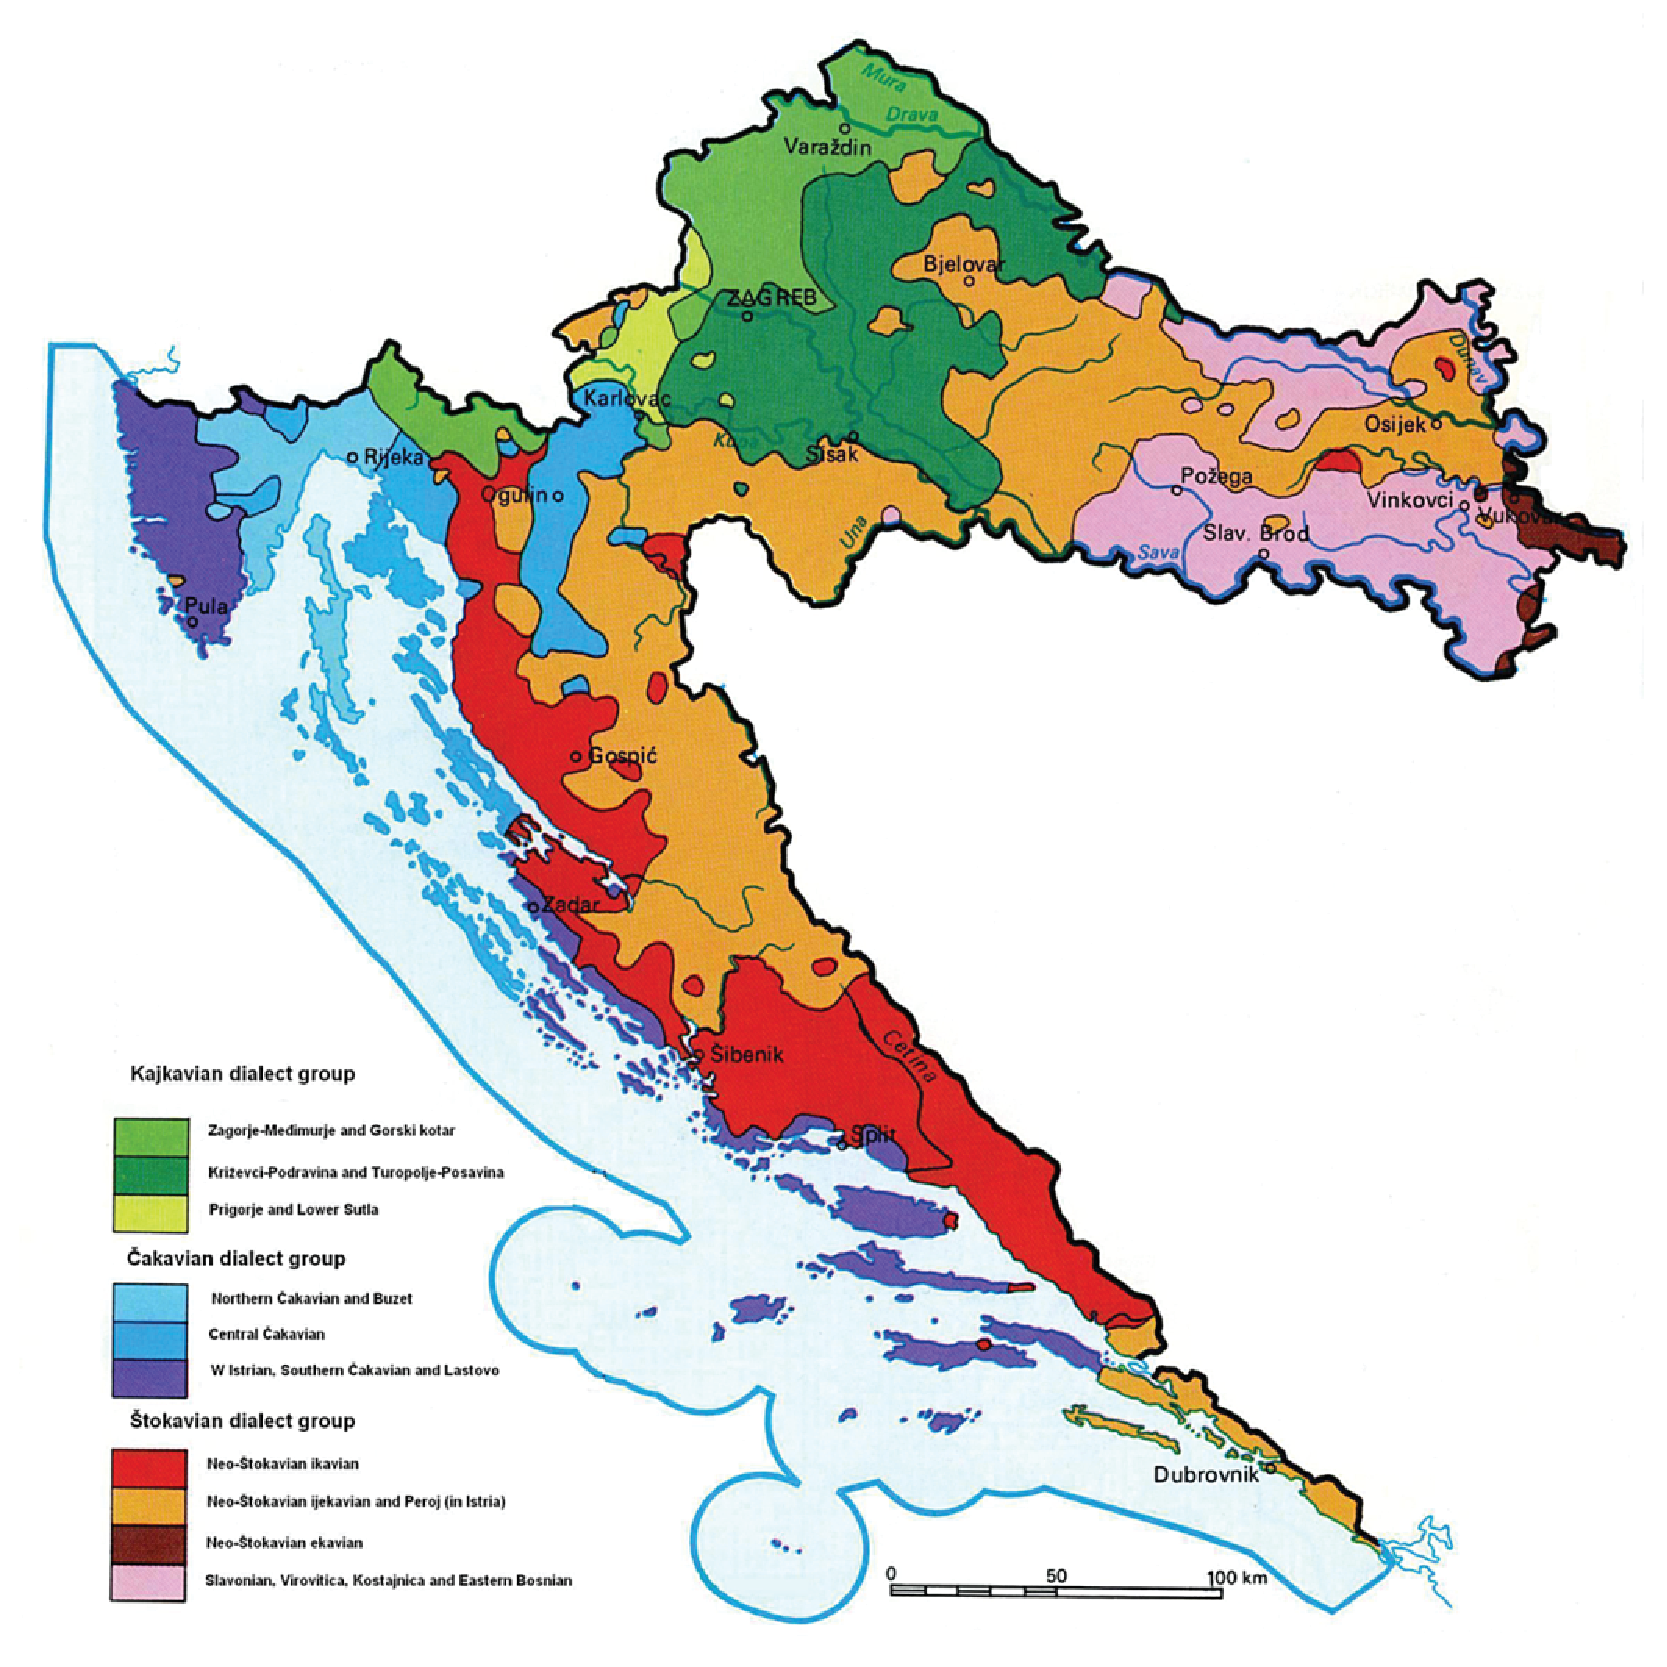
\includegraphics[width=\textwidth]{../_media/croatian/map-dialects}
  \caption{Zemljovid narječja u Republici Hrvatskoj}
  \label{fig:zemljovid}
  \colorrule{grey3}{\textwidth}{1.5pt}
\end{figure*}

\subsection{Standardizacija hrvatskoga jezika}

Tisućljetna povijest hrvatskoga jezika potvrđena je tekstovima pisanim još krajem 10. stoljeća ili početkom 11. stoljeća, u vrijeme kad su se tri hrvatska narječja (čakavski, štokavski i kajkavski) počela oblikovati. Sva su tri hrvatska narječja odigrala važnu ulogu u stvaranju hrvatskoga književnoga jezika (različitih narječnih osnovica) i oblikovanju hrvatske jezične kulture koja je dovela do standardnoga hrvatskoga jezika izgrađenoga na štokavskoj osnovici.

\boxtext{Jeste li znali da je etimologija riječi „kravata“ dolazi od „Croate“ i da se iz francuskoga proširila na ostale jezike u 17. stoljeću?}

Prvi jasni pokušaj oblikovanja hrvatskoga standardnoga jezika pojavio se u 17. stoljeću kad je većina hrvatske etničke zajednice — osobito nakon gramatike i drugih djela Bartola Kašića (1575-1650) i rascvjetale renesansne i barokne književnosti štokavskoga Dubrovnika — prepoznala jezičnu strukturu štokavskoga (isprva s ikavskim refleksom \emph{jata}, ali kasnije s \emph{jekavskim}) kao najbolje polazište za sastavljanje nadregionalnoga hrvatskoga književnoga jezika. Unatoč odabiru jedne jezične osnovice za sastavljanje svoga standardnoga jezika, Hrvati nisu odbacili postignuća višestoljetne jezične kulture različitih narječnih osnovica unutar hrvatskoga književnoga jezika (kajkavsko-štokavsko-čakavski hibrid) koji je obilježio i povijest hrvatske etničke zajednice. Premda je standardizacija jezika Hrvata temeljena na štokavskome narječju započela vrlo rano, narodno se jezično jedinstvo postiglo tek u vrijeme Ilirskoga narodnoga preporoda (počevši od 1835.) kad je mala skupina Hrvata, koji su se do tada služili kajkavskim idiomom, također prihvatili štokavski hrvatski standardni jezik. Tijekom većine 20. stoljeća hrvatski se standardni jezik razvijao u različitim južnoslavenskim državnim jedinicama pod različitim imenima, a bio je predstavljan kao varijanta tzv. hrvatsko-srpskoga (srpsko-hrvatskoga) jezika, ponajprije iz političkih razloga. To je napušteno s demokratskim društveno-političkim promjenama 1990.

Različite stilizacije hrvatskoga jezika oblikovane su još davno u iseljeništvu (npr. gradišćanski hrvatski, moliški hrvatski).
Hrvatska je pisana kultura obilježena uporabom triju pisama (glagoljica, ćirilica, latinica) među kojima je latinica među Hrvatima prevladava od 16. stoljeća. Njezina uporaba nije bila normirana niti usustavljena sve do 1835. kad je Ljudevit Gaj dao hrvatskoj latinici današnji oblik.

\subsection{Osobine hrvatskoga jezika}

\subsubsection{Fonetika, fonologija, morfonologija}

Fonemski inventar hrvatskoga standardnoga jezika sastoji se od 5 samoglasnika (\emph{a, e, i, o, u}) i 25 suglasnika (\emph{m, v, n, l, r, j, nj, lj, p, b, f, s, z, c, t, d, ć, đ, š, ž, č, dž, h, k, g}). Akustične i artikulacijske osobine samoglasnika ne mijenjaju se s obzirom na mjesto izgovora (bez obzira nalazi li se u kratkom, dugom, naglašenom ili nenaglašenom slogu). Uz tih 5 samoglasnika postoji i samoglasničko \emph{r} (\emph{crn} ‘niger’) i dvoglas \emph{ie}, koji se u pismu bilježi kao \emph{je/ije} (\emph{djelo},\emph{odijelo}).

Naglasni sustav sastoji se od 4 naglaska (dva duga naglaska: s uzlaznim i silaznim tonom i dva kratka naglaska: s uzlaznim i silaznim tonom) i zanaglasne dužine. Naglasni je sustav standardnoga hrvatskoga jezika novoštokavski premda danas postoje mnoga odstupanja od naglasnih modela kodificiranih u drugoj polovici 19. stoljeća. Mjesto naglaska nije vezano uz pojedini slog, nego raspodjela naglasaka podliježe stanovitim ograničenjima (npr. zadnji slog višesložne riječi u načelu ne može biti naglašen, silazni naglasci ostvaruju se samo na prvome slogu riječi koje nisu složenice, itd.) Ova se pravila krše u svakodnevnome govoru, osobito u velikim gradskim središtima koja su smještena izvan novoštokavskoga područja (npr. \emph{kontinuitêt} / \emph{kontinuìtēt}). Naglasak i dužina mogu se povremeno rabiti za razlikovanje značenja između leksičkih jedinica ili njihovih oblika, npr. \emph{grȁd : grâd}, \emph{žènē} (gen. jd.) : \emph{žène} (nom. mn.).

U hrvatskome neke riječi nemaju vlastiti naglasak (naslonjenice) već u naglasnoj riječi prednaglasnice mogu preuzeti naglasak prenesen s naglašene riječi ukoliko je naglasak silazni i na prvom je slogu (\emph{grâd} : \emph{ȕ grād}). Kod zanaglasnica to nije moguće. Prenošenje naglaska na prednaglasnicu postaje sve rjeđe, osobito u gradskim središtima izvan neoštokavskoga područja.

U hrvatskome se standardnome jeziku nalaze mnoge fonološki (nom. jd. \emph{sla\textbf{d}ak} : gen. jd. \emph{sla\textbf{t}koga}, nom. jd. dio : gen. jd. \emph{dijela}) i morfonološki uvjetovane promjene (nom. jd. \emph{maj\textbf{k}a} : dat. jd. \emph{maj\textbf{c}i}, nom. jd. \emph{juna\textbf{k}} : vok. jd. \emph{juna\textbf{č}e}).

Regionalna primjena hrvatskoga standardnoga jezika često je u govoru pod utjecajem lokalnoga narječja, npr. na čakavskome Kvarneru prevladava zatvorno \emph{t'} umjesto bezvučnoga poluzatvornoga \emph{ć}, ili u sjeverozapadnome kajkavskome znakovito je nerazlikovanje između \emph{č} – \emph{ć} ili \emph{đ} – \emph{dž}.

\subsubsection{Morfologija}

Hrvatski standardni jezik razlikuje 10 vrsta riječi od kojih su pet promjenljive (imenice, pridjevi, zamjenice, brojevi, glagoli), četiri nepromjenljive (prijedlozi, veznici, uzvici, čestice), a prilozi su promjenljivi samo u komparaciji.

Gramatičke kategorije koje se nalaze u većine promjenljivih riječi jesu rod (tri vrijednosti: muški, ženski, srednji), broj (dvije vrijednosti: jednina, množina), padež (sedam vrijednosti: nominativ, genitiv, dativ, akuzativ, vokativ, lokativ, instrumental). Neke sklonjive riječi imaju i neke posebne kategorije (npr. određenost se obilježava na pridjevima zasebnim nizom flektivnih nastavaka; živo/neživo se obilježava odabirom nastavka za akuzativ jednine imenica muškoga roda; imenice mogu biti konkretne, tvarne, kategorijalne ili zbirne; itd.). Konjugirane riječi (glagoli) obilježene su kategorijama: načina (četiri vrijednosti: indikativ, imperativ, kondicional, optativ), lica (tri vrijednosti: prvo, drugo, treće), broja (dvije vrijednosti: jednina, množina), stanja (dvije vrijednosti: aktiv, pasiv) i vremena (sedam vrijednosti: prezent, imperfekt, aorist, perfekt, pluskvamperfekt, futur I., futur II.). Glagoli \emph{biti} (‘esse’) and \emph{htjeti} (‘volere’) u hrvatskome su pomoćni glagoli. Glagoli također posjeduju složen sustav glagolskih vidova (svršeni i nesvršeni s dodatnim podvrijednostima kao što su početni, učestali itd.), a mogu uključivati i osobinu prijelaznosti. Pridjevi i prilozi mogu se pojaviti i u kompariranim oblicima (tri vrijednosti: pozitiv, komparativ, superlativ).

U hrvatskome postoje dvije osnovne vrste sklonidbe: imenična sklonidba (imenice i neodređeni oblici pridjeva) i zamjenično-pri-djevska sklonidba (zamjenice, određeni oblici pridjeva, brojevi). Svaki imenični rod ima svoju sklonidbu (a-vrsta za muški i srednji rod, e vrsta za ženski), a postoji i posebna i-vrsta (imenice ženskoga roda).

\begin{figure*}[htb]
\centering
	\begin{tabular}{ |l|l|l| }
  \hline
  \textbf{imenična sklonidba} & \textbf{nom. i gen. jd.} & \textbf{nom. mn.}  \\ 
  \hline \hline
  a-vrsta muški rod   & \emph{opis, opis\textbf{a}}     &  \emph{opis\textbf{i}} \\ 
  \hline
  a-vrsta srednji rod   & \emph{sunce, sunc\textbf{a}}     &  \emph{sunc\textbf{a}} \\ 
  \hline
  e-vrsta ženski rod   & \emph{žen\textbf{a}, žen\textbf{e}}     &  \emph{žen\textbf{e}} \\
  \hline
  i-vrsta ženski rod   & \emph{noć, noć\textbf{i}}     &  \emph{noć\textbf{i}} \\
  \hline
  \end{tabular}
  \caption{Imenička sklonidba u hrvatskome jeziku}
  \label{fig:imenicka}
\end{figure*}

Nastavci za zamjenično-pridjevsku sklonidbu prikazani su u ovoj tablici:

\begin{figure*}[htb]
\centering
    \begin{tabular}{|l|l|l|l|}
        \hline
        \textbf{padež} & \textbf{muški rod}         & \textbf{srednji rod}        & \textbf{ženski rod} \\ \hline
		\multicolumn{4}{|c|}{\textbf{jednina}} \\ \hline
        N     & -i                & -o -e             & -a          \\ 
        G     & -og(a) -eg(a)     & -og(a) -eg(a)     & -e          \\ 
        D     & -om(u/e) -em(u/e) & -om(u/e) -em(u/e) & -oj         \\ 
        A     & = N / = G         & = N               & -u          \\ 
        V     & = N               & = N               & = N         \\ 
        L     & -om(u/e) -em(u/e) & -om(u/e) -em(u/e) & = D         \\ 
        I     & -im               & -im               & -om         \\ \hline
		\multicolumn{4}{|c|}{\textbf{množina}} \\ \hline
		N     & -i        & -a         & -e          \\ 
        G     & -ih       & -ih        & -ih         \\ 
        D     & -im(a)    & -im(a)     & -im(a)      \\ 
        A     & -e        & = N        & = N         \\ 
        V     & = N       & = N        & = N         \\ 
        L     & = D       & = D        & = D         \\ 
        I     & = D       & = D        & = D         \\
        \hline
   \end{tabular}
  \caption{Zamjeničko-pridjevska sklonidba u hrvatskome jeziku}
  \label{fig:zamjenicka}
\end{figure*}

Riječi se u hrvatskome tvore derivacijom i slaganjem. Postoji nekoliko različitih načina tvorbe riječi: sufiksalna (\emph{star-ac}), prefiksalno sufiksalna (\emph{do-život-an}), nesufiksalno slaganje (\emph{plačidrug}), sufiksalno slaganje (\emph{vanjskopolitički}), srastanje (\emph{uz-brdo}), slaganje pokrata (\emph{Varteks}) i pretvorba (\emph{mlada}). Najčešća je sufiksalna tvorba.

\subsubsection{Rječnik, frazeologija, nazivlje}

Temeljni se leksički sloj hrvatskoga standardnoga jezika, osim praslavenskoga leksičkoga nasljeđa, sastoji od štokavskoga vokabulara uz primjese vokabulara drugih hrvatskih narječja i vokabulara naslijeđenoga iz književnoga jezika raznih dijalekatnih stilizacija starijega podrijetla (npr. iz kajkavskoga \emph{kukac}, \emph{hlače}, \emph{rječnik}, ili iz čakavskoga \emph{spužva}). Pored toga, cjelina hrvatskoga jezika bila je stalno izložena izravnim ili neizravnim dodirima s drugim jezicima i kulturama. Hrvatski se jezik ističe između ostalih južnoslavenskih jezika znatnim leksičkim utjecajima pristiglim iz romanskih jezika (supstratni tragovi dalmatskoga jezika jesu npr. \emph{jarbol}, \emph{tunj}). Talijanski je jezik bio utjecajan u priobalju (osobito u dijelovima pod negdašnjom mletačkom dominacijom), a njemački i do neke mjere madžarski, u kontinentalnoj Hrvatskoj.

Crkvenoslavenski je književni jezik ostavio tragove u starijim razdobljima hrvatskoga jezika, ali nije imao značajnijega utjecaja tijekom razdoblja u kojem se oblikovao standardni jezik. Ruski jezik nije ostavio tako dubokoga traga u hrvatskome kao što je to učinio u susjednome srpskome standardnome jeziku. Utjecaj vokabulara klasičnih jezika (latinskoga i grčkoga) sveprisutan je u hrvatskoj kulturi, a ponajprije u intelektualnom vokabularu i znanstvenome nazivlju. Tijekom razdoblja srednjohrvatskoga jezika (16.-18. stoljeće) intenzivno su u hrvatski ulazile posuđenice iz turskoga, osobito riječi za predmete iz svakodnevnoga života. Važno je napomenuti kako zbog ranoga iseljavanja, u gradišćanskome hrvatskome nema turskih posuđenica, pa čak niti onih koje se u standardnome hrvatskome više niti ne osjećaju stranim riječima (npr. \emph{bubreg, čizma, jastuk} itd.). Umjesto tih riječi u gradišćanskome hrvatskome rabe se starije hrvatske riječi zajedničkoga slavenskoga podrijetla, te je stoga on vrlo bitan za uvid u povijest hrvatskoga leksičkoga inventara. Njemački i francuski nekad su također utjecali na hrvatski vokabular, a od druge polovice 20. stoljeća utjecaj engleskoga jača. Češki, premda ne u izravnome kontaktu, imao je značajan utjecaj na hrvatski vokabular u nekoliko navrata, osobito tijekom 19. stoljeća za vrijeme izgradnje stručnoga nazivlja koju je bio izveo Bogoslav Šulek (npr. \emph{časopis, kisik, dušik, vodik}). Za vrijeme Jugoslavija, na hrvatski je utjecao i srpski, a osobitu je za to zaslugu imala federalna administracija. Purističke težnje u vokabularu pojavljivale su se od vremena do vremena od 16. do 20. stoljeća (npr. Zoranić, Ritter Vitezović, Reljković, razdoblje 1941.-1945.).

Kontinuitet od davnih vremena do suvremenoga hrvatskoga standardnoga jezika i sudjelovanje triju narječja u izgradnji hrvatskoga standardnoga jezika može se uočiti u njegovoj razvijenoj i bogatoj frazeologiji (npr. u svojim umjetničkim tekstovima iz 16. stoljeća Marulić rabi frazem \emph{zgubiti glas} = 'biti postiđen, izgubiti lice', dok Zoranić rabi frazem u \emph{magnutje oka} = 'odmah', koji su gotovo isti kao frazemi \emph{izgubiti glas} i \emph{u trenu oka} u današnjemu hrvatskome standardnome jeziku temeljenome na štokavskoj osnovici).

Nazivlje u pojedinim stručnim područjima započelo se razvijati već u 16. stoljeću, a to je potvrđeno mnogobrojnim hrvatskim (ponajviše višejezičnim) rječnicima sastavljenim od 16. do 20. stoljeća. U 19. stoljeću njemački i češki imali su iznimno jak utjecaj na hrvatsko nazivlje, a engleski je danas preuzeo tu ulogu.

\subsubsection{Sintaksa}

Hrvatski jezik pripada skupini jezika obilježenih SVO sintaktičkom strukturom (\emph{Marija voli Ivana}) i relativno slobodnim redom riječi (mnogobrojne permutacije sastavnica moguće su uz neka ograničenja kao što je smještaj nenaglasnica). Glede informacijske strukture rečenica, temeljno je pravilo u stilistički neutralnome diskursu da se na prvo mjesto smješta \emph{tema} (stara obavijest), a slijedi u \emph{rema} (nova obavijest, primjedba).

Subjekt u rečenici ne mora biti izrijekom naveden, a njegovo je ispuštanje poželjno ukoliko bi ga se trebalo ponavljati više puta unutar neposredne okoline. Obvezatna je dvostruka negacija (\emph{Nitko ga nije volio}). Sročnost sastavnica u rodu, broju i padežu je tipična za strukturu hrvatskih rečenica. 

U hrvatskome standardnome jeziku postoji sedam padeža, a oblici se mogu kombinirati s prijedlozima (obvezatni uz lokativ). Bitna odrednica hrvatskih glagola jest vid, a glagolski oblici također izražavaju glagolsko vrijeme i modalna značenja. Organizacija složenih rečenica može biti nezavisna ili zavisna (uz prisutnost veznika ili bez njih). Novija je pojava u suvremenome jeziku ograničenje uporabe zajedničkoga slavenskoga genitiva (\emph{Nije volio vina}), posvojne genitivne konstrukcije izbjegavaju se u korist posvojnih pridjeva (\emph{majčina kuća} umjesto \emph{kuća majke}), a uporaba prošlih vremena (imperfekt, aorist i pluskvamperfekt) je sve ograničenija. U suvremenome su hrvatskome pasivne konstrukcije znatno rjeđe nego u starijem hrvatskome.

\subsubsection{Pravopis}

Premda je povijest hrvatske kulture obilježena uporabom triju pisama (glagoljica, ćirilica, latinica), latinica u Hrvata prevladava od 16. stoljeća. Hrvatska latinična abeceda nije bila u cijelosti standardizirana do 1835. kad joj Ljudevit Gaj daje današnji oblik. Sastoji se od 30 slova, od koji su tri dvoslovi (\emph{dž, lj, nj}), a ostala su jednoslovi od čega pet s dijakritičkim znacima (\emph{č, ć, đ, š, ž}). U akademskim krugovima, osobito pri tiskanju tekstova hrvatske pismene baštine, dvoslovi \emph{dž, lj} i \emph{nj} se mogu zamijeniti s \emph{ģ, ļ} and \emph{ń}. Slova \emph{q, x, y, w} ne postoje izvorno u hrvatskoj abecedi premda se rabe za pisanje stranih imena.

\begin{figure*}[htb]
\centering
	\begin{tabular} {|c|c|c|c|c|c|c|c|c|c|c|c|c|c|c|}
        \hline
        \multicolumn{15}{|c|}{\textbf{velika slova}} \\ \hline
        A & B  & C & Č & Ć  & D & DŽ & Đ & E & F & G & H & I & J & K \\ \hline
        L & LJ & M & N & NJ & O & P  & R & S & Š & T & U & V & Z & Ž \\ \hline
        \multicolumn{15}{|c|}{\textbf{mala slova}} \\ \hline
        a & b  & c & č & ć  & d & dž & đ & e & f & g & h & i & j & k \\ \hline
        l & lj & m & n & nj & o & p  & r & s & š & t & u & v & z & ž \\
        \hline
   \end{tabular}
  \caption{Hrvatska latinična abeceda}
  \label{fig:abeceda}
\end{figure*}

Hrvatski je pravopis fonološko-morfonološki jer predstavlja stapanje dvaju pravopisnih načela: nadređenoga fonološkoga (npr. bilježenje asimilacije) i podređenoga morfonološkoga (npr. \emph{podcrtati}). Razmak između riječi je logički, a ne gramatički (kakav je bio nekada). Za hrvatski je pravopis tipično da se pisanje stranih imena ne prilagođuje izgovoru ili grafemskom sastavu hrvatske abecede, a i oblični se nastavci uklapaju u čitavu riječ (npr. \emph{John}, a ne \emph{Džon}; \emph{Washington}, a ne \emph{Vašington}; \emph{Johna}, a ne \emph{John-a}).

\subsubsection{Onomastika}

Hrvatska imena predstavljaju važne spomenike jezičnoga, kulturnoga i društvenoga nasljeđa ljudi koji su ih napravili. Stoga i osobna imena (antroponimi) i imena mjesta (toponimi) čine važan dio hrvatske jezične kulture. Ozemlje današnje Hrvatske, u grubo ograničeno rijekom Dravom na sjeveru, rijekom Dunavom na istoku i Jadranskim morem na jugu, vrlo se ilustrativno reflektira u bogatom raslojavanu zemljopisnih imena.

\boxtext{Jeste li znali kako su Hrvati prvi slavenski\\ narod koji je uveo prezimena u 12. stoljeću?} 

To obilno raslojavanje u hrvatskoj toponimiji odraz je višestoljetnoga suživota različitih etničkih skupina koje su nastanjivale istočnu obalu Jadrana i njezino zaleđe u povijesti. Stoljeća jezičnoga prožimanja i stapanja različitih kulturnih tradicija ostavila su neizbrisiv trag u hrvatskoj toponimiji. Štoviše, potvrđena imena mjesta počesto su svjedocima najstarijih promjena u samome hrvatskome jeziku.

Kako se hrvatski jezik razvijao preko vjerskih (pretkršćanstvo i kršćanstvo), kulturnih i civilizacijskih granica, tragovi i Istoka i Zapada mogu se uočiti u hrvatskim imenima. Kad je riječ o imenima osoba, Hrvati su prvi slavenski narod koji je uveo prezimena (od 12. stoljeća) uzduž jadranske obale uslijed izravnoga romanskoga kulturnoga utjecaja. Najstariji sloj hrvatskih imena oblikovan je u skladu s praslavenskim imenskim obrascima koji su pak slijedili zajedničke indoeuropske obrasce oblikovanja imena. Patronimici još uvijek čine najveći dio inventara prezimena, ali za razliku od ruskoga, danas više nisu produktivni i ostaju neizmijenjeni kao zamrznuta prezimena koja su uklopljena u flektivni sustav kao imenice. U suprotnosti s hrvatskim toponomastičkim sustavom gdje gotovo da i nema turskoga utjecaja, mnoga su hrvatska prezimena oblikovana iz turskih posuđenica hrvatskim tvorbenim nastavcima. Tome je razlog činjenica kako je većina prezimena u Hrvatskoj stvorena nakon tridentinskoga koncila u 16. stoljeću, u vrijeme kad je velik dio hrvatskih zemalja bio pod turskom vlašću.

\subsection{Odnos hrvatskoga standardnoga jezika s ostalim jezicima štokavske osnovice}

Četiri nacionalna jezika, hrvatski, srpski i od nedavna, bošnjački i crnogorski, svi dijele štokavsku strukturnu osnovicu, međutim, tradicije i nadstrukture ovih jezika su poprilično različite. Što razlikuje hrvatsku jezičnu povijest i kulturu od ostalih južnoslavenskih jezika jest odnos između svih triju narječja (kajkavsko, čakavsko, štokavsko) koji odnos postojano obogaćuje hrvatski standardni jezik štokavske osnovice. Zbog različitih polaznih uvjeta (nepostojanje osnovnoga, zajedničkoga standarda) i različitih tradicija u jezičnome kultiviranju i standardizaciji, zbog razjedinjenja neoštokavskih struktura i razlika u jezičnim nadstrukturama jedan zajednički monolitni standarni jezik nikad nije bio uspio biti oblikovan tijekom postojanja jugoslavenskih država, premda je postojalo nekoliko pokušaja političkoga nametanja zajedničkoga imena jezika (\emph{srpsko-hrvatsko-slovenački} za Kraljevine Jugoslavije; \emph{srpsko-hrvatski} ili \emph{hrvatsko-srpski} za komunističke Jugoslavije). Za vrijeme Drugoga svjetskoga rata i nekoliko godina nakon njega svi su službeni dokumenti u Jugoslaviji objavljivani na četiri službena jezika (hrvatskome, makedonskome, slovenskome, srpskome), no ubrzo je mnogo po-litičkoga napora uporabljeno za ponovnu konvergenciju hrvatskoga i srpskoga. Unatoč svim pokušajima da se službeno prizna postojanje hrvatskoga kao zasebnoga jezika, nametanje zajedničkoga nazivlja, vokabulara, pravopisa i drugih jezičnih normi u Jugoslaviji, dovelo je jedino do službenoga prihvaćanja jednoga zajedničkoga standardnoga jezika (\emph{srpsko-hrvatskoga}) s dvije varijante (\emph{istočnom ili srpskom} i \emph{zapadnom ili hrvatskom}). Reakcija iz Hrvatske došla je ubrzo u obliku \emph{Deklaracije o nazivu i položaju hrvatskog knjževnog jezika} koja se otvoreno zalagala za priznavanje samostalnoga hrvatskoga jezika i koju su jednoglasno 1967. potpisale vodeće znanstvene, kulturne i obrazovne ustanove, kao i vodeći intelektualci diljem Hrvatske, a koji su se tako otvorenim političkim potezom nesumnjivo doveli u opasnost u komunističkim vremenima.

Tijekom zadnjih 20 godina, četiri štokavski temeljena standardna jezika razvijaju se samostalno kao nacionalni standardni jezici u prirodno divergentnim smjerovima budući da ne postoji nikakav sporazum ili koordinacija glede njihovoga zajedničkoga normiranja, pa su se time među njima razlike uvećale.

\subsection{Skrb o jeziku u Hrvatskoj}

Vijeće za normu hrvatskoga standardnoga jezika ustanovljeno je odlukom Ministarstva znanosti, obrazovanja i športa, 14. travnja 2005. Njegova je temeljna zadaća sustavna i znanstveno utemeljena skrb o hrvatskome standardnome jeziku. Posebni zadatci Vijeća su:

\begin{itemize}
\item skrb o hrvatskome standardnome jeziku;
\item raspravljati o aktualnim nedoumicama i otvorenim pitanjima hrvatskoga standardnog jezika;
\item upozoravati na primjere nepoštivanja ustavne odredbe o hrvatskome kao službenome jeziku u Republici Hrvatskoj;
\item promicati kulturu hrvatskoga standardnog jezika u pisanoj i govornoj komunikaciji;
\item skrbiti o statusu i ulozi hrvatskoga standardnoga jezika u svjetlu integracije Hrvatske u Europsku uniju;
\item donositi odluke u daljnjem procesu standardizacije hrvatskoga standardnoga jezika;
\item brinuti o jezičnim pitanjima i postavljati načela za pravopisnu standardizaciju.
\end{itemize}

Vijeće za normu hrvatskoga standardnoga jezika sastaje se redovite i kroz temeljite rasprave dolazi do zaključaka. Institut za hrvatski jezik i jezikoslovlje udomljuje Vijeće, pruža mu tehničku i administrativnu podršku kao i jezikoslovne savjete kad je to potrebno.
Institut za hrvatski jezik i jezikoslovlje \cite{str7} središnja je hrvatska ustanova za istraživanje hrvatskoga jezika, a jedan je od njegovih odjela (Odjel za hrvatski standardni jezik) posvećen opisu hrvatskoga standardnoga jezika s osobitom pozornošću na jezičnu kulturu (npr. pružanje javnosti jezičnih savjeta ili pisanje jezičnih priručnika). Savjeti o ispravnoj jezičnoj uporabi i jezikoslovna ekspertiza stalne su dužnosti Instituta. Savjeti se daju telefonski, e-poštom ili u pisanome obliku. Uz to, odgovori na najčešće postavljana pitanja dostupni su na portalu Jezični savjeti \cite{str8} u sastavu institutova www-sjedišta.

\boxtext{Temeljna je zadaća Vijeća za normu\\ hrvatskoga standardnoga jezika sustavna i znanstveno utemeljena skrb o hrvatskome standardnome jeziku.}

Institutov projekt STRUNA \cite{str9}, unutar kojega se razvija hrvatsko stručno nazivlje zaslužuje posebno spominjanje. Cilj je ovoga projekta uspostava sustava koordinacije terminoloških poslova u svim stručnim područjima u Hrvatskoj i time pripomoći poboljšanju kakvoće i učinkovitosti višega obrazovanja i znanstvenih istraživanja izgradnjom jedinstvenoga provjerenoga nazivlja koje mogu rabiti stručnjaci svih polja, a i zainteresirani pojedinci i opće javnosti. Također se planira uspostava mreže istraživačkoga nazivlja kao i znanstvena suradnja između ustanova koje se bave različitim vidovima terminološkoga rada.

\boxtext{Danas su posuđenice iz engleskoga jezika česte u govornome, a rjeđe u hrvatskome pisanom jeziku.}

Pored toga, ostale hrvatske znanstvene ustanove (nekoliko sveučilišta s njihovim odsjecima za hrvatski jezik i književnost) i kulturne ustanove (kao što je \emph{Matica hrvatska}) također sudjeluju u skrbi o hrvatskome jeziku. Javna glasila, kao što su državna radio-televizija i neki novinski nakladnici imaju dobro razvijene korektorske i lektorske službe za hrvatski standardni jezik, te obraćaju posebnu pozornost na kakvoću jezika koji rabe u svojoj proizvodnji javno dostupnih tekstova.

\subsection{Jezik u obrazovanju}

Hrvatski je jezik služben u svim osnovnim i srednjim školama osim u područjima s pučanstvom nacionalnih manjina. Međutim, nije određen kao obvezatan na sveučilištima. Premda u Hrvatskoj postoje težnje, posebice u prirodnim znanostima, da se predavanja održavaju na engleskome jeziku, koje se težnje opravdavaju tvrdnjama kako je to svrhovito i korisno, sasvim je jasno da bi bilo iznimno štetno i neprihvatljivo ne poučavati na hrvatskome na sveučilištima. To bi imalo razarajući učinak na razvoj hrvatskoga znanstvenoga nazivlja i stručne frazeologije. Stoga je Vijeće za normu hrvatskoga standardnoga jezika preporučilo Ministarstvu da službeno odredi uporabu jezika u visokome obrazovanju.

U osnovnim i srednjim školama Hrvatski jezik i književnost poučava se kao predmet koji zauzimlje značajan dio školskih sati. Kao dio toga predmeta proučava se hrvatska gramatika, rječnik i književnost, a razvijaju se također pismeno i govorno izražavanje na hrvatskome jeziku. PISA testiranje, koje provjerava vještine učenika na svjetskoj razini, provodi se u Hrvatskoj od 2006, a prvi rezultati provjera pokazuju kako hrvatski petnaestogodišnjaci zauzimaju 26. mjesto na ljestvici svih zemalja svijeta i smješteni su ispred učenika iz deset zemalja-članica EU i SAD.

U osnovnim i srednjim školama uz hrvatski obvezatno je učenje barem jednoga stranoga jezika od četvrtoga razreda. Međutim, engleski se jezik (rijetko francuski ili njemački) nerijetko uče već u dječjem vrtiću. Engleski je uobičajeno prvi strani jezik u osnovnoj školi. Najrašireniji drugi strani jezik je njemački, potom slijede talijanski i francuski. U srednjim školama ponekad se uče ruski i španjolski kao drugi ili treći strani jezik. Latinski i starogrčki uče se u klasičim programima koji počinju u petome razredu osnovne škole. K tome je latinski obvezatan u svim humanističkim srednjim školama. U školi židovske manjine (koja ima pravo javnosti), moguće je učiti i hebrejski. Obrazovanje na manjinskim jezicima dostupno je od dječjega vrtića do srednje škole i hrvatska ga Vlada financira za srpsku, češku, madžarsku i talijansku manjinu.

\subsection{Međunarodni odnosi}

Uporaba hrvatskoga standardnoga jezika u zemljama regije regulirana je zakonima tih zemalja. Status hrvatskoga standardnoga jezika kao jednoga od službenih jezika susjedne Bosne i Hercegovine od osobite je važnosti, pa hrvatske ustanove posvećuju osobitu pozornost suradnji sa znanstvenim i kulturnim ustanovama hrvatskoga naroda u Bosni i Hercegovini. Također, kulturne ustanove iz Republike Hrvatske uspostavljaju suradnju s mnogim hrvatskim iseljeničkim ustanovama diljem svijeta.

\boxtext{Kad Republika Hrvatska pristupi Europskoj\\ uniji u 2013., hrvatski će jezik postati 24. službeni jezik EU.}

Poučavanje hrvatskoga jezika organizirano je u inozemnim školama za djecu hrvatskih državljana koji privremeno ili trajno žive u drugim zemljama. Hrvatski se jezik poučava na mnogim inozemnim ustanovama i u središtima za slavenske jezike (tako postoji 36 službenih razmjenskih lektorata za hrvatski jezik i književnosti kao i dva središta za Hrvatske studije u Australiji i Kanadi koje sve podupire Ministarstvo znanosti, obrazovanja i športa Republike Hrvatske). Velik broj središta za učenje hrvatskoga kao drugoga ili stranoga jezika postoji u Hrvatskoj, a najpoznatiji je \emph{Croaticum} \cite{str10}.

\subsection{Hrvatski na Internetu}

Statistika Državnoga zavoda za statistku o uporabi informacijskih i komunikacijskih tehnologija u poduzećima i kućanstvima dana je u sljedećoj tablici:

\begin{figure*}[htb]
\centering
    \begin{tabular}{|c|c|c|c|}
        \hline
      \multicolumn{4}{|c|}{\textbf{Uporaba informacijskih i komunikacijskih tehnologije (ICT) u poduzećima (\%)}} \\ \hline
        ~                                              & 2008 & 2009 & 2010 \\ \hline
        \emph{uporaba računala}                        & 98   & 98   & 97   \\ \hline
        \emph{pristup Internetu}                       & 97   & 95   & 95   \\ \hline
        \emph{www-sjedište}                            & 64   & 57   & 61   \\ \hline
        \emph{uporaba financijskih i bankovnih usluga} & 84   & 84   & 85   \\ \hline
        \emph{uporaba usluga e-uprave}                 & 56   & 61   & 63   \\
        \hline
   \end{tabular}
  \caption{ICT u poduzećima}
  \label{fig:IST_pod}
\end{figure*}

\begin{figure*}[htb]
\centering
	\begin{tabular}{|c|c|c|c|}
        \hline
      \multicolumn{4}{|c|}{\textbf{Kućanstva opremljena informacijskim i komunikacijskim tehnologijama (ICT) (\%)}} \\ \hline
        ~                                              & 2008 & 2009 & 2010 \\ \hline
        \emph{osobno računalo}   & 53   & 55   & 60   \\ \hline
        \emph{pristup Internetu} & 45   & 50   & 57   \\ \hline
        \emph{mobilni telefon}   & 81   & 82   & -    \\
        \hline
   \end{tabular}
  \caption{ICT u kućanstvima}
  \label{fig:IST_kuc}
\end{figure*}

Najposjećenija hrvatska www-sjedišta su: \emph{net.hr} (portal za vijesti, sport, zabavu i zbivanja), \emph{index.hr} (opći www-portal, informacije, usluge, vijesti, sport, zabava, vozila, gastronomija), \emph{jutarnji.hr} (www sjedište dnevnih novina“Jutarnji list”), \emph{24sata.hr} (www-sjedište dnevnih novina “24 sata”), \emph{tportal.hr} (portal HT-a, Hrvatskih telekomunikacija), \emph{njuskalo.hr} (“Njuškalo” portal s oglasima), \emph{vecernji.hr} (www-sjedište dnevnih novina “Večernji list”), \emph{forum.hr} (najveći hrvatski www-forum na kojem se raspravlja o temama iz društva, kulture, zabave itd.). Sedam dnevnih novina svakodnevno objavljuje svoje članke i na vlastitim www-sjedištima pored papirnatih izdanja.

\boxtext{Rastuća uloga Interneta važna\\ je i za jezične tehnologije.}

Institut za hrvatski jezik i jezikoslovlje održava www-stranicu o hrvatskome jeziku koja donosi iscrpan popis hrvatskih jedno- i višejezičnih rječnika, gramatika i pravopisnih priručnika. Na Filozofskome fakultetu Sveučilišta u Zagrebu održava se slična www stranica \cite{str11}. Na istome se fakultetu od 1999. održava i portal Jezične tehnologije za hrvatski jezik \cite{str12}.
Wikipedija na hrvatskome jeziku osnovana je 2003. i trenutačno broji 100.708 članaka, te je 30. Wikipedija po službenome broju članaka.

Pristup jezičnim resursima za hrvatski jezik u zadnje je vrijeme olakšan zbog broja hrvatskih ustanova i organizacije koje provode postupke digitalizacije (uključujući značajne projekte koje podupire Ministarstvo znanosti, obrazovanja i športa i Ministarstvo kulture u digitalizaciji hrvatske kulturne baštine), a koja je uvećala vidljivost hrvatskoga jezika među ostalim internetskim izvorima.
\end{multicols}

\clearpage

% --------------------------------------------------------------------------

\ssection[Jezičnotehnološka podrška za hrvatski]{Jezičnotehnološka podrška za hrvatski}

\begin{multicols}{2}
Jezične se tehnologije koriste za razvoj sustava namijenjenih za obradbu prirodnoga jezika, te se mogu pojaviti i pod nazivom „prirodnojezične tehnologije“. Prirodni se jezik pojavljuje u govorenom i pisanom obliku. Dok je govor najstariji i najprirodniji oblik jezičnoga priopćavanja, složene obavijesti i većina ljudskoga znanja sadržana je i prenosi se s pomoću teksta. Govorne tehnologije i tehnologije obradbe teksta obrađuju jezik u ovim dvama načinima njegova ostvaraja služeći se rječnicima, gramatičkim pravilima i značenjem. To znači da jezične tehnologije povezuju jezik s različitim oblicima znanja, neovisno o mediju (govoreni ili pisani tekst) u kojem se ostvaruje. Slika ~\ref{fig:ltincontext_cro} prikazuje okružje jezičnih tehnologija.

U našem priopćavanju miješamo jezik s ostalim oblicima priopćavanja i drugim medijima, npr. govor uključuje gestikulaciju i mimiku. Digitalni tekst povezujemo sa slikama i zvukovima. U filmovima se jezik pojavljuje u govorenom i pisanom obliku. Stoga se govorne tehnologije i tehnologije obradbe teksta preklapaju i prožimaju se s mnogim drugim tehnologijama koje pospješuju obradbu multimedijskoga priopćavanja i multimedijskih tehnologija.

U ovome ćemo poglavlju prikazati glavna područja primjene jezičnih tehnologija, kao što su jezična provjera, www-tražilice, govorna interakcija i strojno prevođenje. Te aplikacije i temeljnje tehnologije uključuju:
\begin{itemize}
\item provjeru pravopisa
\item potpora stvaranju tekstova
\item računalno potpomognuto učenje jezika
\item pretraga obavijesti
\item crpljenje obavijesti
\item sažimanje teksta
\item odgovaranje na pitanja
\item prepoznavanje govora
\item generiranje govora
\end{itemize}

\begin{figure*}[htb]
  \colorrule{grey3}{\textwidth}{1.5pt}
  \center
  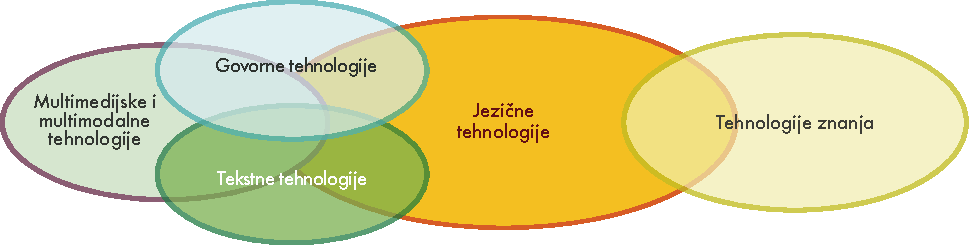
\includegraphics[width=\textwidth]{../_media/croatian/language_technologies}
  \caption{Jezične tehnologije}
  \label{fig:ltincontext_cro}
  \colorrule{grey3}{\textwidth}{1.5pt}
\end{figure*}

Jezične su tehnologije već čvrsto uspostavljeno zasebno istraživačko područje s širokim rasponom uvodne literature. Zainteresirani čitatelj se upućuje na sljedeće referencije: \cite{pro12, boo7, boo8, str37, boo9}.

Prije nego što krenemo prikazivati navedena područja istraživanja, na kratko bismo opisali arhitekturu uobičajenoga jezičnotehnološkoga sustava.

\subsection{Arhitekture jezičnotehnoloških aplikacija}

Uobičajena se programska aplikacija za obradbu jezika sastoji od nekoliko dijelova koji se bave različitim jezičnim slojevima. Dok takve aplikacije mogu biti vrlo složene, slika ~\ref{fig:textprocessingarch_cro} pokazuje znatno pojednostavnjenu arhitekturu kakva se može naći u sustavima za obradbu teksta. Prva tri modula bave se strukturom i značenjem ulaznoga teksta:

\begin{figure*}[b]
  \colorrule{grey3}{\textwidth}{1.5pt}
  \center
  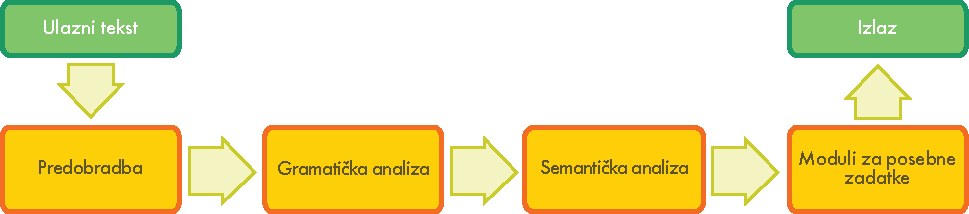
\includegraphics[width=\textwidth]{../_media/croatian/text_processing_app_architecture}
  \caption{Tipična aplikacija za obradu teksta}
  \label{fig:textprocessingarch_cro}
  \colorrule{grey3}{\textwidth}{1.5pt}
\end{figure*}

\begin{enumerate}
\item predobradba: čišćenje ulaznih podataka, analiza i uklanjanje oblikovanja teksta, određivanje ulaznoga jezika, ponekad umetanje nedostajućih dijakritičkih znakova u hrvatskome, itd.
\item gramatička raščlamba: pronalaženje glagola i njegovih objekata, subjekata, njihovih atributa itd.; prepoznavanje rečenične strukture.
\item semantička raščlamba: razobličenje (npr. koje značenje riječi „glava“ je primjereno u danom kontekstu?), razrješenje anafore (određivanje na što se točno odnosne zamjenice kao što su „ona“, „kojemu“, itd. u tekstu odnose); predstavljanje značenje rečenice u strojno čitljivome obliku.
\end{enumerate}

Nakon te analize zadatkovno-orijentirani moduli izvode mnoge specifične postupke kao što su npr. automatsko sažimanje ulaznoga teksta, pretraga baza podataka i mnoge druge.

Nakon uvodnoga dijela o osnovim područjima primjene jezičnih tehnologija, dat će se kratak pregled stanja jezičnih tehnologija u istraživanjima i obrazovanju koji će se zaključiti pregledom prošlih, sadašnjih i budućih istraživačkih programa razvoja jezičnih tehnologija za hrvatski jezik \cite{boo5}. Na kraju ovoga poglavlja prikazat će se stručna procjena stanja osnovnih jezičnih resursa i alata za hrvatski jezik sagledanoga kroz niz kategorija kao što su dostupnost, zrelost ili kakvoća. Opće stanje jezičnih tehnologija za hrvatski jezik je sažeto u obliku tablice. Najvažniji resursi i alati koji se opisuju u tekstu su dani masnim slovima, a može ih se također naći u tablici ~\ref{fig:resursi_cro} na kraju poglavlja. Jezične tehnologije za hrvatski jezik uspoređene su i s jezičnim tehnologijama za druge jezicima uključene u niz ovih bijelih knjiga.

\subsection{Osnovna područja primjene jezičnih tehnologija} 

\subsubsection{Jezična provjera}

Svatko tko koristi obradnike teksta kao što je npr. Microsoft Word, naišao je pravopisni provjernik koji obilježava pogrješke u tipkanju i predlaže ispravke. Prvi pravopisni provjernici uspoređivali su riječi iz teksta s rječnikom ispravno napisanih riječi. Danas su ovi programi znatno razrađeniji. Uz dodatak jezično ovisnih algoritama za obradbu morfologije (npr. prepoznavanje različitih padeža), neki već mogu prepoznati i sintaktičke pogrješke kao što je ispuštanje glagola ili nesročnost između subjekta i predikata u broju i rodu, npr. „Ona je *pisao pismo.“ Pa ipak, i najnapredniji provjernici ne mogu pronaći pogrješke u prvoj strofi pjesme Jerrolda H. Zara (1992):

\begin{figure*}[t]
  \colorrule{grey3}{\textwidth}{1.5pt}
  \center
  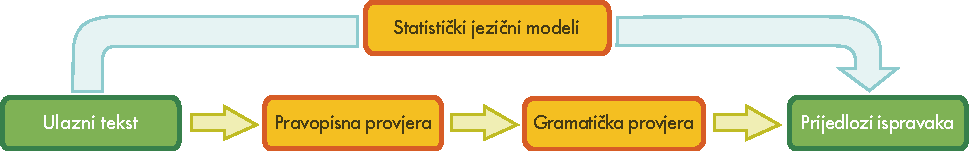
\includegraphics[width=\textwidth]{../_media/croatian/language_checking}
  \caption{Tipična aplikacija za jezičnu provjeru}
  \label{fig:langcheckingaarch_cro}
  \colorrule{grey3}{\textwidth}{1.5pt}
\end{figure*}

\begin{itemize}
\item[] I have a spelling checker,\\
  It came with my PC.\\
  It plane lee marks four my revue\\
  Miss steaks aye can knot sea.
\end{itemize}

Za razrješivanje ovakvih pogrješaka u mnogim je slučajevima potrebna raščlamba konteksta, npr. treba li u hrvatskome imenicu pisati velikim  (žensko osobno ime) ili malim (opća imenica) početnim slovom kao u slučaju:

\begin{itemize}
\item \textbf{Slatka je ova višnja.}.\\
  {[}This cherry is sweet.{]} 
\item \textbf{Slatka je ova Višnja.}.\\
  {[}This Cherry is sweet.{]}
\end{itemize}

Takva raščlamba zahtijeva bilo oblikovanje jezično posebnih \textbf{gramatičkih pravila}, izradba kojih uključuje visoku stručnost i mnogo radnih sati, ili uporabu tzv. statističkih jezičnih modela. Takvim je modelima točno izračunana vjerojatnost pojavljivanja neke riječi u određenome kontekstu (tj. s obzirom na prethodeću ili slijedeću riječ). Na primjer, u hrvatskome je \textbf{jaz između} mnogo češći niz dviju riječi nego \textbf{jaz generacija}. Statistički se jezični model može proizvesti automatski iz velike količine (ispravnih) jezičnih podataka (tj. iz \textbf{korpusa}). Do sada su se ova dva pristupa mahom razvila i provjerila na jezičnim podatcima za engleski jezik. Međutim, na hrvatski jezik takva rješenja nisu izravno primjenljiva zbog njegove bogate fleksije i slobodnijega reda riječi u rečenici koji u mnogome pridonose takvim sustavima problematičnoj raspršenosti podataka.

Uporaba jezičnih provjernika nije ograničena samo na obradnike teksta, već se koristi i u potpornim alatima za stvaranje teksta kao što su opsežni priručnici i ostala tehnička dokumentacija kad je riječ o primjeni računalnih sustava u informacijskim tehnologijama, zdravstvu, strojarstvu i drugdje. Bojeći se korisničkih pritužaba o pogrješnoj uporabi ili odštetnih zahtjeva zbog nepreciznih ili loše shvaćenih korisničkih uputa, tvrtke se sve više okreću prema stvaranju što kvalitetnijih korisničkih uputa i tehničke dokumentacije dok se istodobno pokušavaju širiti na međunarodnome tržištu (kroz prevođenje i lokalizaciju). Napredak u računalnoj obradbi prirodnoga jezika doveo je do razvoja potpornih programa za pisanje teksta koji pomažu piscima tehničke dokumentacije pri uporabi kontroliranoga jezika u kojem je u skladu s (korporativnim) pravilima ograničena uporaba leksičkih jedinica, stručnoga nazivlja ili jednostavijih sintaktičkih struktura. Za hrvatski takvi alati još nisu na raspolaganju.

\boxtext{Jezični provjernici nisu ograničeni samo\\ na obradnike teksta, već se koriste i u potpornim alatima za stvaranje teksta.}

Premda su istraživanja računalnih modela hrvatske flektivne morfologije postojala još u 1980-ima, prvi je komercijalni prvopisni provjernik \emph{Hrvatski računalni pravopis} objavljen tek 1996. \cite{boo2} Ubrzo ga je preuzeo Microsoft i danas je sastavni dio Microsoft Officea te je u najširoj uporabi. Nekoliko je privatnih tvrtki također razvilo pravopisne provjernike, ali niti jedan nije bio toliko uspješan. \emph{On-line Hrvatski akademski spelling checker} (Hascheck) \cite{str13} postoji od 1994 i još uvijek je u uporabi. Za hrvatski također postoji i besplatni prvopisni provjernik temeljem na ispell/aspell aplikaciji, a uporabiv je na svim platformama na kojima je dostupan OpenOffice. Svi se ovi programi temelje na vrlo velikim leksikonima ispravno napisanih riječi, a taj pristup ima dvije osnovne manjkavosti: 1) nizovi pismena koji predstavljaju ispravno napisane riječi mogu se pojaviti u pogrješnome kontekstu; 2) nemogućnost prepoznavanja ispravno napisanih riječi koje su nepoznate leksikonu. Osim provjernika pravopisa i potpornih programa za stvaranje teksta, jezična je provjera važna i na području strojno potpomognutoga učenja jezika, a primjenjuje se i kod automatskoga ispravljanja upita poslanih www-tražilicama, npr. Googleove „Jeste li mislili...“ preporuke. 

\subsubsection{WWW tražilice}

Pretraga na mreži, na intranetima ili u digitalnim knjižnicama danas je vjerojatno najšire korištena, a ipak još nedovoljno razvijena, jezična tehnologija. Tražilica Google, koja je započela 1998., danas se rabi za otprilike 80\% svih pretraga u svijetu \cite{str14}. Od 2004. u hrvatskome se koristi glagol guglati/googlati i njegove tvorenice (\emph{iz-/na-/pre-/pro-/u-})guglati/(\emph{iz-/na-/pre-/pro-/u-})googlati premda si još nije izborio mjesto u tiskanim rječnicima (zabilježeni su čak i složenije tvorenice kao npr. ugugljiv). Ni sučelje za pretragu, niti prikaz dohvaćenih rezultata nisu se značajno promijenili od prve inačice. U trenutačnoj inačici Google nudi pravopisnu provjeru za pogrješno napisane riječi, a uključuje u pretragu i osnovne semantičke elemente kojima je moguće poboljšati točnost pretrage analizom značenja upita u danome kontekstu \cite{str15}. Uz pomoć ovoga algoritma Google je počeo pokrivati hrvatske riječi u nekima od oblika u kojima se pojavljuju u tekstu. Za razliku od npr. engleskih imenica gdje postoje samo četiri moguća oblika (\emph{hand, hand’s, hands, hands’}), hrvatske se teoretski mogu pojaviti u 14 različitih oblika, ali su prosječno predstavljeni s 10 različitih nizova (\emph{ruka, ruke, ruci, ruku, rukom, rukama}...). Googleova tražilica može pronaći oblike kao što su \emph{ruka} ili \emph{ruke}, ali oblik \emph{ruci} već nije više povezan uz imenicu \emph{ruka}. Ima još dosta prostora za poboljšanja u Googleovoj tražilici kod flektivno bogatih jezika kod kojih se mora nositi s činjenicom da se pojedine riječi mogu pojaviti u većem broju oblika. Međutim, uspjeh Googlea pokazuje kako s golemim količinama podataka i učinkovitim tehnikama njihova indeksiranja, pretežito statistički utemeljeni pristup može dovesti do zadovoljavajućih rezultata, no njihova kakvoća također ovisi i o samoj strukturi prirodnoga jezika na kojem se pretražuje.

\begin{figure*}[htb]
  \colorrule{grey3}{\textwidth}{1.5pt}
  \center
  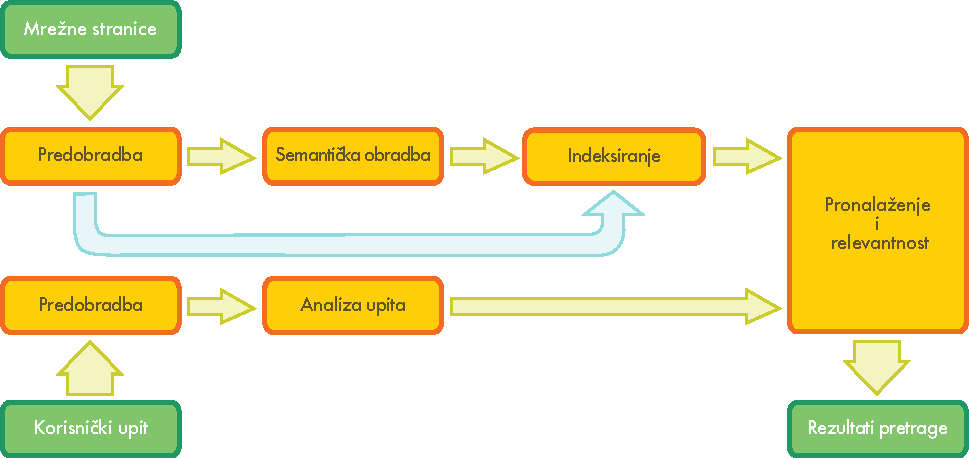
\includegraphics[width=\textwidth]{../_media/croatian/web_search_architecture}
  \caption{Arhitektura www-tražilice}
  \label{fig:websearcharch_cro}
  \colorrule{grey3}{\textwidth}{1.5pt}
\end{figure*}

Pa ipak, za razrađenije pretrage obavijesti uključivanje dubljega jezičnoga znanja bit će ključno za ispravnu interpretaciju rezultata. Eksperimenti u kojim se rabe \textbf{leksički resursi} kao što su strojno čitljivi tezaurusi i ontološki organizirani jezični resursi (npr. WordNet za engleski ili Hrvatski Wordnet – CroWN) pokazuju ozbiljan napredak omogućujući pronalaženje www-stranica na temelju sinonima upitnih riječi, npr. \emph{nuklearna energija} i \emph{atomska energija} ili na temelju riječi još udaljenije povezanih s upitnim riječima.

\boxtext{Sljedeći će naraštaj tražilica morati uključivati razrađenije jezične tehnologije.} 

Pa ipak, za razrađenije pretrage obavijesti uključivanje dubljega jezičnoga znanja bit će ključno za ispravnu interpretaciju rezultata. Eksperimenti u kojim se rabe leksički resursi kao što su strojno čitljivi tezaurusi i ontološki organizirani jezični resursi (npr. WordNet za engleski ili Hrvatski Wordnet – CroWN) pokazuju ozbiljan napredak omogućujući pronalaženje www-stranica na temelju sinonima upitnih riječi, npr. nuklearna energija i atomska energija ili na temelju riječi još udaljenije povezanih s upitnim riječima.

Sljedeći će naraštaj tražilica morati uključivati razrađenije jezične tehnologije, osobito ako upit bude sadržavao pitanje ili kakvu drugu rečenicu umjesto popisa upitnih riječi.  Za upit \emph{Daj mi popis svih tvrtki koje su bile preuzete od drugih tvrtki u zadnjih pet godina}, potrebna je sintaktička i \textbf{semantička analiza}. Sustav također mora žurno priskrbiti i tako indeksirane dokumente. Za zadovoljavajući odgovor na ovo pitanje potrebna je primjena sintaktičke raščlambe (parsanja) kako bi se raščlanila sintaktička struktura rečenice i odredilo kako korisnik traži tvrtke koje je neka tvrtka preuzela, a ne tvrtke koje su preuzele neku tvrtku. Također, izraz \emph{u zadnjih pet godina}, treba obraditi kako bi se odredilo o kojih je točno pet godina riječ uzimajući u obzir tekuću godinu. Konačno, obrađeni upit se mora sraziti s golemom količinom nestrukturiranih podataka kako bi se pronašao komadić ili komadići obavijesti koje korisnik traži. Taj se zadatak obično naziva pretraga obavijesti i uključuje pretragu i rangiranje relevantnih dokumenata. K tome pri sastavljanju zahtijevanoga popisa tvrtki, sustav mora moći prepoznati u pretraživanim dokumentima kako određen niz pismena doista predstavlja ime tvrtke. Takav se zadatak zove prepoznavanje imena i obavlja ga specijalizirana aplikacija za tu namjenu. Još su zahtjevniji pokušaji da se na temelju upita pronađu relevantni dokumenti pisani na drugim jezicima. Za takvo višejezično pretraživanje obavijesti moramo strojno prevesti upit na se moguće jezike i pronađene dokumente prevesti na jezik upita.

Rastuća količina podataka dostupnih u netekstnim oblicima potiče stvaranje usluga koje bi omogućile multimedijsko pretraživanje obavijesti, npr. pretragu u slikovnim, audio- ili video-zapisima. Za audio- i video-zapise još je potreban i modul za raspoznavanje govora koji bi omogućio pretvorbu govora u tekst ili njegov fonetski zapis u kojem se onda može obavljati pretraga.

Za flektivno bogate jezike kao što je hrvatski, tražilice moraju omogućiti pretragu odjednom po svim oblicima u kojima se neka riječ može pojaviti, umjesto da se svaki oblik mora unositi pojedinačno. Takav oblik pretrage moguće je izvesti s pomoću Hrvatskoga lematizacijskoga poslužitelja koji je razvijen na Odsjeku za lingvistiku Filozofskoga fakulteta Sveučilišta u Zagrebu i slobodno je dostupan preko Interneta \cite{str16} omogućujući pristup Hrvatskome morfološkome leksikonu, opsežnoj bazi podataka hrvatskih riječi i svih njihovih oblika. Ta baza sadrži preko 110.000 natuknica iz kojih je generirano preko 4 milijuna oblika tako da svaki zapis u bazi sadrži natuknicu, oblik i MSD-oznaku tj. popis svih gramatičkih kategorija koje su se ostvarile tim oblikom. Taj je zapis usklađen s MulText East \cite{str17} preporukama.

Godine 2009., kao rezultat zajeničkoga flamansko-hrvatskoga projekta CADIAL \cite{str18}, vladina agencija HIDRA omogućila je javni www-pristup svim hrvatskim zakonskim i podzakonskim dokumentima putem flektivno osjetljive tražilice \cite{str19}. Ta tražilica takođe omogućuje i višejezičnu pretragu dokumenata s obzirom na to da su svi dokumenti indeksirani deskriptorima iz EUROVOC-a što omogućuje uporabu i engleskih deskriptora u upitu.
  
\subsubsection{Govorna interakcija}

Govorna interakcija jedno je od mnogih područja primjene govornih tehnologija, tj. tehnologija za obradbu govora. Tehnologije za govornu interakciju stvaraju sučelja koja omogućuju komunikaciju govorenoga jezika umjesto grafičkoga sučelja, tipkovnice ili miša. Danas su takva govorna korisnička sučelja (\emph{voice user interfaces}, VUI) uključena u djelomično ili potpuno automatizirane usluge koje razne tvrtke nude svojim korisnicima, zaposlenicima ili partnerima putem telefona. Područja koja danas u mnogome ovise o uporabi VUI-ja su bankarstvo, logistika, javni prijevoz i telekomunikacije. Drugi oblici uporabe tehnologija za govornu interakciju su sučelja prema pojedinim uređajima, npr. sustavi za cestovnu navigaciju ili sustavi gdje je govorna interakcija zamjena za ulazno/izlazne podatke grafičkih sučelja, npr. kod pametnih telefona.

\begin{figure*}[htb]
  \colorrule{grey3}{\textwidth}{1.5pt}
  \center 
  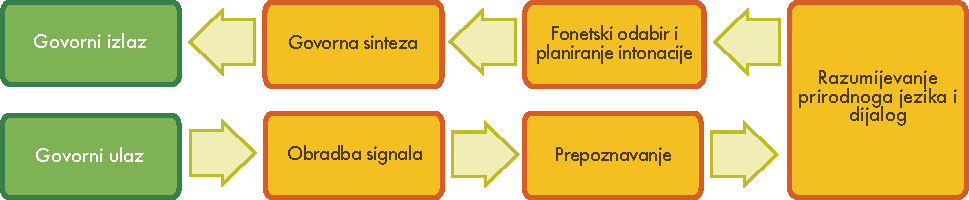
\includegraphics[width=\textwidth]{../_media/croatian/simple_speech-based_dialogue_architecture}
  \caption{Govorna interakcija}
  \label{fig:dialoguearch_cro}
  \colorrule{grey3}{\textwidth}{1.5pt}
\end{figure*}

Sustavi koji koriste tehnologiju za govornu interakciju sastoje se od četiri različita podsustava s pripadajućim tehnologijama:

\begin{enumerate}
\item Automatsko \textbf{prepoznavanje govora} (\emph{automatic speech recognition}, ASR) određuje koje su riječi zaista izgovorene u nizu glasova koje je korisnik izrekao.
\item Razumijevanje prirodnoga jezika bavi se analizom sintaktičke strukture korisnikova iskaza i njegovom interpretacijom u skladu s namjenom određenoga sustava.
\item Upravljanje razgovorom određuje koju akciju sustav mora poduzeti na temelju korisničkove upute i na temelju ukupne funkcionalnosti toga sustava.
\item \textbf{Sinteza govora} (\emph{text-to-speech}, TTS) tehnologija se rabi za pretvaranje pojedinih riječi nekoga iskaza u niz glasova koji će biti odaslani korisniku. 
\end{enumerate}

\boxtext{Govorna interakcija je temelj za stvaranje sučelja koja omogućuju korisniku uporabu govora umjesto grafičkoga sučelja, tipkovnice i miša.}

Jedan od glavnih izazova jest kako da ASR-sustav što točnije prepozna riječi koje je korisnik uporabio. To zahtijeva ili ograničenje broja mogućih korisničkih iskaza na ograničen skup riječi, ili ručno stvaranje jezičnoga modela koji pokriva širok raspon mogućih iskaza na prirodnome jeziku. Uporabom postupaka strojnoga učenja jezični se modeli mogu automatski generirati iz \textbf{govornih korpusa}, tj. velikih zbirki govornih audio snimaka i njihove tekstovne transkripcije. Ograničavanje skupa dopuštenih iskaza obično ne omogućuje korisnicima uporabu VUI-ja na prirodan način, pa takvi sustavi znaju korisnicima izgledati i zvučati odbojno. Istodobno, sastavljanje, podešavanje i održavanje takvih opsežnih jezičnih i govornih modela znatno poskupljuje takve sustave. S druge strane sustavi koji rabe jezične modele, već u polasku dopuštaju korisnika slobodnije izražavanje, npr. započinjanjem razgovora rečenicom „Kako vam mogu pomoći?“, pokazuju i viši stupanj automatizacije i viši stupanj korisničkoga prihvaćanja.

Za određene dijelove VUI-ja, tvrtke nerijetko rabe snimljene iskaze profesionalnih spikera. Tako snimljeni statični iskazi, u kojima se riječi ne mijenjaju ovisno o kontekstu uporabe ili o osobnim podatcima pojedinoga korisnika, korisniku mogu pružiti kvalitetu govora koju očekuje. Međutim, što je sadržaj dinamičniji, tada je i vjernost govora manja jer je potrebno umjetno povezivati velik broj malih snimki. Nasuprot ovim sustavima, današnje sustave za TTS moguće je podešavati do željene kakvoće s obzirom na prirodnost naglaska dinamično organiziranih iskaza.

U proteklom je desetljeću na tržištu tehnologija za govornu interakciju došlo do uznapredovale standardizacije sučeljavanja različitih tehnoloških komponenta. Također je u proteklome desetljeću došlo do značajnoga okrupnjivanja na tržištu, osobito kad je riječ o ASR i TTS sustavima. Na tržištima u zemljama skupine G20 tj. gospodarski jakih zemalja značajne populacije, prevladava pet svjetski relevantnih tvtrki, s tim što su Nuance (SAD) i Loquendo (Italija) najzastupljenije u Europi. Godine 2011. Nuance je najavio preuzimanje Loquenda što će značiti daljnji korak u okrupnjavanju tržišta.

Premda je baza hrvatskih difona razvijena još 1998. unutar projekta MBROLA \cite{str20} u kojem je sudjelovao Odsjek za fonetiku Filozofskoga fakulteta Sveučilišta u Zagrebu, do danas još uvijek ne postoji niti jedan komercijalni sustav za hrvatski ATS ili TTS razvijen u Hrvatskoj. Istraživanja na ovome području provode se i na Fakultetu elektrotehnike i računarstva istoga sveučilišta \cite{art1}, ali i na Sveučilištu u Rijeci jaka skupina istraživača radi na razvoju resursa i alata za obradbu hrvatskoga govora \cite{art2, str21, art3}.

Ako bi se pokušao baciti pogled onkraj sadašnjega stanja ove tehnologije, mogle bi se očekivati značajne promjene s obzirom na ubrzano širenje pametnih telefona kao nove platforme za odnose s korisnicima uz već postojeće kao što su telefon, Internet i e-pošta. Ovakav se razvoj prilika može očekivati i u slučaju primjene tehnologije za govornu interakciju. S jedne će strane i dugoročno gledano potrebe za klasičnim telefonskim VUI zacijelo opadati, a s druge će strane uporaba govora kao izvora ulaznih podataka za pametne telefone zacijelo biti u porastu. Taj smjer razvoja također se može prepoznati s obzirom na vidan napredak točnosti prepoznavanja govora neovisnoga o govorniku u sustavima za diktiranje koji se već nude kao usluga korisnicima pametnih telefona.

\subsubsection{Strojno prevođenje}

Zamisao uporabe računala za prevođenje s jednoga prirodnoga jezika na drugi može se smjestiti još u 1946., a uslijedila joj je značajna potpora za istraživanja u tom području tijekom 1950-ih i ponovno u 1980-ima. Pa ipak, \textbf{strojno prevođenje} (\emph{machine translation}, MT) još uvijek ne uspijeva ispuniti visoka očekivanja glede njegove kakvoće. 

\boxtext{U svom najjednostavnijem obliku MT\\ samo zamjenjuje riječi jednoga prirodnoga\\ jezika riječima iz drugoga.}

Najjednostavniji oblik strojnoga prevođenja sastoji se od zamjene riječi jednoga prirodnoga jezika riječima iz drugoga. To može biti uporabivo u uskim područjima s izrazito ograničenim, formulaičnim izrazima, npr. kod vremenskih izvješća. Međutim, za dobar prijevod manje ograničenih tekstova, veći tekstni odsječci (fraze, rečenice ili čitavi odlomci) moraju se što više u prijevodu približiti svojim prijevodnim ekvivalentima u polaznome jeziku. Najveći je problem u tome što je prirodni jezik višeznačan, a taj se problem pojavljuje na više razina, npr. na razini razobličenja značenja riječi (word sense disambiguation, WSD) na leksičkoj razini (Jaguar na početku rečenice može značiti životinju ili automobilsku marku) ili na razini smještanja prijedložnoga izraza u sintaktičkoj strukturi kao u primjeru:

\begin{itemize}
\item Policajac je uočio čovjeka bez teleskopa.\\
  {[}The policeman spotted a man without a telescope.{]} 
\item Policajac je uočio čovjeka bez pištolja.\\
  {[}The policeman spotted a man without a pistol.{]}
\end{itemize}

Jedan od mogućih pristupa izgradnji strojnoprevoditeljskih sustava temeljen je na jezičnim pravilima. Za prevođenje između bliskosrodnih jezika, izravno bi prevođenje moglo biti lakše izvedivo. Nerijetko sustavi temeljeni na pravilima (ili na jezičnome znanju) raščlanjuju ulazni tekst i pretvaraju ga u posrednu simboličku prezentaciju iz koje se onda generira tekst na ciljnome jeziku. Uspjeh ovakvih pristupa u mnogome ovisi o dostupnim opsežnim rječnicima s morfološkim, sintaktičkim i semantičkim podatcima, ali i o velikom broju gramatičkih pravila koje su brižljivo izradili visokostručni jezikoslovci. To je vrlo zahtjevan, dugotrajan i stoga skup posao.

\begin{figure*}[htb]
  \colorrule{grey3}{\textwidth}{1.5pt}
  \center
  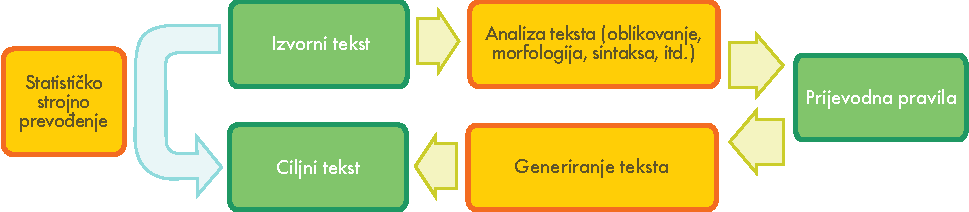
\includegraphics[width=\textwidth]{../_media/croatian/machine_translation}
  \caption{Statističko strojno prevođenje}
  \label{fig:mtarch_cro}
  \colorrule{grey3}{\textwidth}{1.5pt}
\end{figure*}

S krajem 1980-ih, kad je porasla snaga računala i kad su ona postala dostupnija, više se zanimanja počelo posvećivati statističkim modelima u strojnome prevođenju. Statistički modeli izvedeni su iz raščlambe dvojezičnih korpusa tj. \textbf{usporednih korpusa} kao što je npr. Europarl korpus, koji sadrži zapisnike sjednica Europskoga parlamenta na 21 europskih jezika, ili JRC-Acquis usporedni korpus \cite{pro6} na 22 europska jezika. Kad im se osigura dovoljno podataka, statistički sustavi za strojno prevođenje rade dovoljno dobro za dobivanje približnoga značenja teksta na stranome jeziku obradbom usporednih tekstova i pronalaženjem odgovarajućih prijevodnih podudarnosti među njima. Međutim, za razliku od sustava temeljenih na znanju (ili pravilima), MT sustavi temeljeni na statistici (ili podatcima) često generiraju tekst koji nije ovjeren tj. nije usklađen s gramatikom ciljnoga jezika. Podatkovno temeljeni pristupi strojnome prevođenju su u prednosti jer zahtijevaju manje ljudskoga napora, a mogu pokriti i osobitosti jezika (npr. idiomatske izraze) koje obično sustavi temeljeni na pravilima zanemaruju ili zaobilaze. Kad se gledaju samo europski jezici, prihvatljivi se prijevodi mogu dobiti za engleski i romanske jezike, no kakvoća prijevoda značajno opada za ostale germanske, slavenske, ugrofinske ili baltičke jezike \cite{pro2}.

\boxtext{Strojno je prevođenje osobito izazovno za slavenske jezike zbog njihova slobodnoga reda riječi, bogatstva oblika riječi i postojanja udaljenih a međuovisnih dijelova iste fraze.}
 
Kako su prednosti i nedostatci sustava za strojno prevođenje temeljenih na znanju i sustava temeljenih na podatcima upravo komplementarno raspoređeni, danas se istraživači mahom usmjeravaju na hibridne pristupe koji kombiniraju metodologije obiju vrsta ovih sustava. Jedan od načina hibridizacije jest uporaba obje vrste sustava za obavljanje prevođenja, a potom selekcijski modul odlučuje o tome koji je rezultat više kakvoće za svaku pojedinu rečenicu. Na žalost, u slučaju duljih rečenica, npr. više od 12 riječi, niti jedan sustav još uvijek ne daje prijevod željene kakvoće. Učinkovitijim se doima pristup u kojem se kombiniraju najbolji dijelovi rečenica iz višestrukih mogućih prijevoda, a oni mogu biti poprilično složeni s obzirom da odgovarajući dijelovi višestrukih prijevodnih rješenja nisu uvijek lako uočljivi, te se moraju posebno sravnjivati. 

Strojno je prevođenje s i na hrvatski jezik osobito izazovan zadatak. Slobodniji red riječi u rečenici i bogata fleksija predstavljaju probleme pri generiranju ispravnih rečeničnih konstrukcija i oblika riječi koji obličnim nastavcima kodiraju gramatičke kategorije roda, padeža, broja, načina, vremena itd. Dodatne probleme često postavlja i zahtjev za sročnošću glede tih kategorija između npr. atributa i imenice u rodu, broju i padežu ili samo u rodu i broju kad je riječ o subjektu i predikatu.

Premda su Željko Bujas i Bulcsú László još 1959. organizirali prvu radionicu o strojnome prevođenju \cite{art4} na Filozofskome fakultetu Sveučilišta u Zagrebu, nikakvo ozbiljnije istraživanje o strojnome prevođenju za hrvatski jezik nije se dogodilo prije 21. stoljeća. Projekt „Informacijske tehnologije u prevođenju i e-učenju hrvatskoga“ \cite{str22} pokrenut je 2007. s ciljem istraživanja koji su preduvjeti potrebni za stvaranje MT sustava za prevođenje na i s hrvatskoga jezika. Počevši od 2010. Europska je komisija pokrenula i potpomaže nekoliko projekata kako bi se razvila istraživanja i razvoj strojnoga prevođenja za tzv. jezike s nedovoljno razvijenim resursima, a među njih je uključen i hrvatski. Tako CIP ICT PSP projekt LetsMT! \cite{str23} i FP7 projekt ACCURAT \cite{str24} razvijaju nove metode za što jednostavnije prikupljanje podataka potrebnih za strojno prevođenje i izgradnju takvih sustava prilagođenih različitim domenama i oblicima primjene. U oba ova projekta kao hrvatski partner sudjeluje skupina istraživača s Filozofskoga fakulteta Sveučilišta u Zagrebu.

Projekt ACCURAT \cite{pro3} istražuje nove metode uporabe usporedivih korpusa ne bi li se nadoknadila nestašica jezičnih resursa i posredno poboljšalo strojno prevođenje za jezike s nedovoljnim resursima i za uske domene \cite{pro4}. Cilj je projekta ACCURAT postići značajan napredak u kakvoći strojnoga prijevoda za čitav niz novih službenih jezka EU i jezika zemalja-pristupnica (estonski, grčki, hrvatski, letonski, litavski i rumunjski), kao i predložiti nove pristupe za prilagodbu tehnologija za strojno prevođenje u pojedinim uskim domenama i time značajno povećati pokrivenost različitih jezika i domena strojnim prevođenjem.

Projekt LetsMT! \cite{pro5} izgrađuje novi vrstu \emph{on-line} suradne platforme za dijeljenje usporednih tekstova i automatsko stvaranje vlastitih sustava za strojno prevođenje. Ova platforma smještena u računalnome oblaku omogućit će svim vrstama korisnika slanje u posebno zaštićen repozitorij vlastitih jezičnih resursa na temelju kojih će se potom automatski izraditi vlastiti sustav za statističko strojno prevođenje treniran upravo na temelju tih vlastitih jezičnih resursa. Takav sustav za strojno prevođenje potom se može podijeliti s ostalim korisnicima. Strojnoprevoditeljske usluge projekta LetsMT! mogu se rabiti na nekoliko načina: kroz www-portal, kroz \emph{widget} koji se može slobodno preuzeti i uključiti na svoje www-stranice, kroz dodatak za popularne prebirnike kao i kroz integraciju u postojeće sustave za strojno potpomognuto prevođenje kako \emph{on-line}, tako i \emph{off-line}.

Google Translate nudi prijevode na hrvatski i s hrvatskoga od 2008. Kakvoća njegovih prijevoda bila je niska u početku, ali se poboljšava kako je sve više i više usporednih hrvatsko-engleskih podataka dostupno \emph{on-line}.

Još uvijek se smatra kako upravo na području poboljšanja kakvoće prijevoda ima još mnogo prostora za napredak kod sustava za strojno prevođenje. Napredak se očekuje u prilagodbi jezičnih resursa određenom području uporabe ovisno o temi ili korisniku, kao i u integraciji s postojećim sustavima za strojno potpomognuto prevođenje u kojima se već rabe velike terminološke baze i prijevodne memorije. Dodatni je problem što je većina trenutačnih strojnoprevoditeljskih sustava usmjerena na engleski i podupire svega još nekoliko jezika pri prevođenju na hrvatski i s hrvatskoga. To zapravo onemogućuje druge prijevodne smjerove, a istodobno zahtijeva od korisnika da se služe većim brojem raznorodnih sustava.

Postupci vrjednovanja omogućuju uspoređivanje kakvoće prijevoda sustava za strojno prevođenje, njihove različite pristupe i stanje strojnoprevoditeljskih sustava za različite jezike. U okviru projekta Euromatrix+ sastavljena je ~\ref{fig:euromatrix_en} u kojoj je prikazana kakvoća za sve parove strojnih prijevoda između 22 službena jezika EU-a (irski jedino nedostaje) iskazana s pomoću BLEU mjere \cite{pro6} koja s većim brojem bodova iskazuje višu kakvoću prijevoda. Ljudski prevoditelji obično postižu oko 80 bodova. 

\begin{figure*}[htbp]
  \centering
  \setlength{\tabcolsep}{0.17em}
  \small
  \begin{tabular}{>{\columncolor{corange1}}cccccccccccccccccccccccc}
    & \multicolumn{22}{>{\columncolor{corange1}}c}{Markmál -- \textcolor{grey1}{Target language}}\\\addlinespace[{-.009cm}]
    \rowcolor{corange1}  & EN & BG & DE & CS & DA & EL & ES & ET & FI & FR & HU & IT & LT & LV & MT & NL & PL & PT & RO & SK & SL & SV\\
    EN & -- & \textcolor{blue}{40.5} & \textcolor{blue}{46.8} & \textcolor{green2}{52.6} & \textcolor{green2}{50.0} & \textcolor{blue}{41.0} & \textcolor{green2}{55.2} & \textcolor{purple}{34.8} & \textcolor{purple}{38.6} & \textcolor{green2}{50.1} & \textcolor{purple}{37.2} & \textcolor{green2}{50.4} & \textcolor{purple}{39.6} & \textcolor{blue}{43.4} & \textcolor{purple}{39.8} & \textcolor{green2}{52.3} & \textcolor{blue}{49.2} & \textcolor{green2}{55.0} & \textcolor{blue}{49.0} & \textcolor{blue}{44.7} & \textcolor{green2}{50.7} & \textcolor{green2}{52.0}\\
    BG & \textcolor{green}{61.3} & -- & \textcolor{purple}{38.7} & \textcolor{purple}{39.4} & \textcolor{purple}{39.6} & \textcolor{purple}{34.5} & \textcolor{blue}{46.9} & \textcolor{red3}{25.5} & \textcolor{red3}{26.7} & \textcolor{blue}{42.4} & \textcolor{red3}{22.0} & \textcolor{blue}{43.5} & \textcolor{red3}{29.3} & \textcolor{red3}{29.1} & \textcolor{red3}{25.9} & \textcolor{blue}{44.9} & \textcolor{purple}{35.1} & \textcolor{blue}{45.9} & \textcolor{purple}{36.8} & \textcolor{purple}{34.1} & \textcolor{purple}{34.1} & \textcolor{purple}{39.9}\\
    DE & \textcolor{green2}{53.6} & \textcolor{red3}{26.3} & -- & \textcolor{purple}{35.4} & \textcolor{blue}{43.1} & \textcolor{purple}{32.8} & \textcolor{blue}{47.1} & \textcolor{red3}{26.7} & \textcolor{red3}{29.5} & \textcolor{purple}{39.4} & \textcolor{red3}{27.6} & \textcolor{blue}{42.7} & \textcolor{red3}{27.6} & \textcolor{purple}{30.3} & \textcolor{red2}{19.8} & \textcolor{green2}{50.2} & \textcolor{purple}{30.2} & \textcolor{blue}{44.1} & \textcolor{purple}{30.7} & \textcolor{red3}{29.4} & \textcolor{purple}{31.4} & \textcolor{blue}{41.2}\\
    CS & \textcolor{green2}{58.4} & \textcolor{purple}{32.0} & \textcolor{blue}{42.6} & -- & \textcolor{blue}{43.6} & \textcolor{purple}{34.6} & \textcolor{blue}{48.9} & \textcolor{purple}{30.7} & \textcolor{purple}{30.5} & \textcolor{blue}{41.6} & \textcolor{red3}{27.4} & \textcolor{blue}{44.3} & \textcolor{purple}{34.5} & \textcolor{purple}{35.8} & \textcolor{red3}{26.3} & \textcolor{blue}{46.5} & \textcolor{purple}{39.2} & \textcolor{blue}{45.7} & \textcolor{purple}{36.5} & \textcolor{blue}{43.6} & \textcolor{blue}{41.3} & \textcolor{blue}{42.9}\\
    DA & \textcolor{green2}{57.6} & \textcolor{red3}{28.7} & \textcolor{blue}{44.1} & \textcolor{purple}{35.7} & -- & \textcolor{purple}{34.3} & \textcolor{blue}{47.5} & \textcolor{red3}{27.8} & \textcolor{purple}{31.6} & \textcolor{blue}{41.3} & \textcolor{red3}{24.2} & \textcolor{blue}{43.8} & \textcolor{red3}{29.7} & \textcolor{purple}{32.9} & \textcolor{red3}{21.1} & \textcolor{blue}{48.5} & \textcolor{purple}{34.3} & \textcolor{blue}{45.4} & \textcolor{purple}{33.9} & \textcolor{purple}{33.0} & \textcolor{purple}{36.2} & \textcolor{blue}{47.2}\\
    EL & \textcolor{green2}{59.5} & \textcolor{purple}{32.4} & \textcolor{blue}{43.1} & \textcolor{purple}{37.7} & \textcolor{blue}{44.5} & -- & \textcolor{green2}{54.0} & \textcolor{red3}{26.5} & \textcolor{red3}{29.0} & \textcolor{blue}{48.3} & \textcolor{red3}{23.7} & \textcolor{blue}{49.6} & \textcolor{red3}{29.0} & \textcolor{purple}{32.6} & \textcolor{red3}{23.8} & \textcolor{blue}{48.9} & \textcolor{purple}{34.2} & \textcolor{green2}{52.5} & \textcolor{purple}{37.2} & \textcolor{purple}{33.1} & \textcolor{purple}{36.3} & \textcolor{blue}{43.3}\\
    ES & \textcolor{green}{60.0} & \textcolor{purple}{31.1} & \textcolor{blue}{42.7} & \textcolor{purple}{37.5} & \textcolor{blue}{44.4} & \textcolor{purple}{39.4} & -- & \textcolor{red3}{25.4} & \textcolor{red3}{28.5} & \textcolor{green2}{51.3} & \textcolor{red3}{24.0} & \textcolor{green2}{51.7} & \textcolor{red3}{26.8} & \textcolor{purple}{30.5} & \textcolor{red3}{24.6} & \textcolor{blue}{48.8} & \textcolor{purple}{33.9} & \textcolor{green2}{57.3} & \textcolor{purple}{38.1} & \textcolor{purple}{31.7} & \textcolor{purple}{33.9} & \textcolor{blue}{43.7}\\
    ET & \textcolor{green2}{52.0} & \textcolor{red3}{24.6} & \textcolor{purple}{37.3} & \textcolor{purple}{35.2} & \textcolor{purple}{37.8} & \textcolor{red3}{28.2} & \textcolor{blue}{40.4} & -- & \textcolor{purple}{37.7} & \textcolor{purple}{33.4} & \textcolor{purple}{30.9} & \textcolor{purple}{37.0} & \textcolor{purple}{35.0} & \textcolor{purple}{36.9} & \textcolor{red3}{20.5} & \textcolor{blue}{41.3} & \textcolor{purple}{32.0} & \textcolor{purple}{37.8} & \textcolor{red3}{28.0} & \textcolor{purple}{30.6} & \textcolor{purple}{32.9} & \textcolor{purple}{37.3}\\
    FI & \textcolor{blue}{49.3} & \textcolor{red3}{23.2} & \textcolor{purple}{36.0} & \textcolor{purple}{32.0} & \textcolor{purple}{37.9} & \textcolor{red3}{27.2} & \textcolor{purple}{39.7} & \textcolor{purple}{34.9} & -- & \textcolor{red3}{29.5} & \textcolor{red3}{27.2} & \textcolor{purple}{36.6} & \textcolor{purple}{30.5} & \textcolor{purple}{32.5} & \textcolor{red2}{19.4} & \textcolor{blue}{40.6} & \textcolor{red3}{28.8} & \textcolor{purple}{37.5} & \textcolor{red3}{26.5} & \textcolor{red3}{27.3} & \textcolor{red3}{28.2} & \textcolor{purple}{37.6}\\
    FR & \textcolor{green}{64.0} & \textcolor{purple}{34.5} & \textcolor{blue}{45.1} & \textcolor{purple}{39.5} & \textcolor{blue}{47.4} & \textcolor{blue}{42.8} & \textcolor{green}{60.9} & \textcolor{red3}{26.7} & \textcolor{purple}{30.0} & -- & \textcolor{red3}{25.5} & \textcolor{green2}{56.1} & \textcolor{red3}{28.3} & \textcolor{purple}{31.9} & \textcolor{red3}{25.3} & \textcolor{green2}{51.6} & \textcolor{purple}{35.7} & \textcolor{green}{61.0} & \textcolor{blue}{43.8} & \textcolor{purple}{33.1} & \textcolor{purple}{35.6} & \textcolor{blue}{45.8}\\
    HU & \textcolor{blue}{48.0} & \textcolor{red3}{24.7} & \textcolor{purple}{34.3} & \textcolor{purple}{30.0} & \textcolor{purple}{33.0} & \textcolor{red3}{25.5} & \textcolor{purple}{34.1} & \textcolor{red3}{29.6} & \textcolor{red3}{29.4} & \textcolor{purple}{30.7} & -- & \textcolor{purple}{33.5} & \textcolor{red3}{29.6} & \textcolor{purple}{31.9} & \textcolor{red2}{18.1} & \textcolor{purple}{36.1} & \textcolor{red3}{29.8} & \textcolor{purple}{34.2} & \textcolor{red3}{25.7} & \textcolor{red3}{25.6} & \textcolor{red3}{28.2} & \textcolor{purple}{30.5}\\
    IT & \textcolor{green}{61.0} & \textcolor{purple}{32.1} & \textcolor{blue}{44.3} & \textcolor{purple}{38.9} & \textcolor{blue}{45.8} & \textcolor{blue}{40.6} & \textcolor{red3}{26.9} & \textcolor{red3}{25.0} & \textcolor{red3}{29.7} & \textcolor{green2}{52.7} & \textcolor{red3}{24.2} & -- & \textcolor{red3}{29.4} & \textcolor{purple}{32.6} & \textcolor{red3}{24.6} & \textcolor{green2}{50.5} & \textcolor{purple}{35.2} & \textcolor{green2}{56.5} & \textcolor{purple}{39.3} & \textcolor{purple}{32.5} & \textcolor{purple}{34.7} & \textcolor{blue}{44.3}\\
    LT & \textcolor{green2}{51.8} & \textcolor{red3}{27.6} & \textcolor{purple}{33.9} & \textcolor{purple}{37.0} & \textcolor{purple}{36.8} & \textcolor{red3}{26.5} & \textcolor{red3}{21.1} & \textcolor{purple}{34.2} & \textcolor{purple}{32.0} & \textcolor{purple}{34.4} & \textcolor{red3}{28.5} & \textcolor{purple}{36.8} & -- & \textcolor{blue}{40.1} & \textcolor{red3}{22.2} & \textcolor{purple}{38.1} & \textcolor{purple}{31.6} & \textcolor{purple}{31.6} & \textcolor{red3}{29.3} & \textcolor{purple}{31.8} & \textcolor{purple}{35.3} & \textcolor{purple}{35.3}\\
    LV & \textcolor{green2}{54.0} & \textcolor{red3}{29.1} & \textcolor{purple}{35.0} & \textcolor{purple}{37.8} & \textcolor{purple}{38.5} & \textcolor{red3}{29.7} & \textcolor{red2}{8.0} & \textcolor{purple}{34.2} & \textcolor{purple}{32.4} & \textcolor{purple}{35.6} & \textcolor{red3}{29.3} & \textcolor{purple}{38.9} & \textcolor{purple}{38.4} & -- & \textcolor{red3}{23.3} & \textcolor{blue}{41.5} & \textcolor{purple}{34.4} & \textcolor{purple}{39.6} & \textcolor{purple}{31.0} & \textcolor{purple}{33.3} & \textcolor{purple}{37.1} & \textcolor{purple}{38.0}\\
    MT & \textcolor{green}{72.1} & \textcolor{purple}{32.2} & \textcolor{purple}{37.2} & \textcolor{purple}{37.9} & \textcolor{purple}{38.9} & \textcolor{purple}{33.7} & \textcolor{blue}{48.7} & \textcolor{red3}{26.9} & \textcolor{red3}{25.8} & \textcolor{blue}{42.4} & \textcolor{red3}{22.4} & \textcolor{blue}{43.7} & \textcolor{purple}{30.2} & \textcolor{purple}{33.2} & -- & \textcolor{blue}{44.0} & \textcolor{purple}{37.1} & \textcolor{blue}{45.9} & \textcolor{purple}{38.9} & \textcolor{purple}{35.8} & \textcolor{blue}{40.0} & \textcolor{blue}{41.6}\\
    NL & \textcolor{green2}{56.9} & \textcolor{red3}{29.3} & \textcolor{blue}{46.9} & \textcolor{purple}{37.0} & \textcolor{blue}{45.4} & \textcolor{purple}{35.3} & \textcolor{blue}{49.7} & \textcolor{red3}{27.5} & \textcolor{red3}{29.8} & \textcolor{blue}{43.4} & \textcolor{red3}{25.3} & \textcolor{blue}{44.5} & \textcolor{red3}{28.6} & \textcolor{purple}{31.7} & \textcolor{red3}{22.0} & -- & \textcolor{purple}{32.0} & \textcolor{blue}{47.7} & \textcolor{purple}{33.0} & \textcolor{purple}{30.1} & \textcolor{purple}{34.6} & \textcolor{blue}{43.6}\\
    PL & \textcolor{green}{60.8} & \textcolor{purple}{31.5} & \textcolor{blue}{40.2} & \textcolor{blue}{44.2} & \textcolor{blue}{42.1} & \textcolor{purple}{34.2} & \textcolor{blue}{46.2} & \textcolor{red3}{29.2} & \textcolor{red3}{29.0} & \textcolor{blue}{40.0} & \textcolor{red3}{24.5} & \textcolor{blue}{43.2} & \textcolor{purple}{33.2} & \textcolor{purple}{35.6} & \textcolor{red3}{27.9} & \textcolor{blue}{44.8} & -- & \textcolor{blue}{44.1} & \textcolor{purple}{38.2} & \textcolor{purple}{38.2} & \textcolor{purple}{39.8} & \textcolor{blue}{42.1}\\
    PT & \textcolor{green}{60.7} & \textcolor{purple}{31.4} & \textcolor{blue}{42.9} & \textcolor{purple}{38.4} & \textcolor{blue}{42.8} & \textcolor{blue}{40.2} & \textcolor{green}{60.7} & \textcolor{red3}{26.4} & \textcolor{red3}{29.2} & \textcolor{green2}{53.2} & \textcolor{red3}{23.8} & \textcolor{green2}{52.8} & \textcolor{red3}{28.0} & \textcolor{purple}{31.5} & \textcolor{red3}{24.8} & \textcolor{blue}{49.3} & \textcolor{purple}{34.5} & -- & \textcolor{purple}{39.4} & \textcolor{purple}{32.1} & \textcolor{purple}{34.4} & \textcolor{blue}{43.9}\\
    RO & \textcolor{green}{60.8} & \textcolor{purple}{33.1} & \textcolor{purple}{38.5} & \textcolor{purple}{37.8} & \textcolor{blue}{40.3} & \textcolor{purple}{35.6} & \textcolor{green2}{50.4} & \textcolor{red3}{24.6} & \textcolor{red3}{26.2} & \textcolor{blue}{46.5} & \textcolor{red3}{25.0} & \textcolor{blue}{44.8} & \textcolor{red3}{28.4} & \textcolor{red3}{29.9} & \textcolor{red3}{28.7} & \textcolor{blue}{43.0} & \textcolor{purple}{35.8} & \textcolor{blue}{48.5} & -- & \textcolor{purple}{31.5} & \textcolor{purple}{35.1} & \textcolor{purple}{39.4}\\
    SK & \textcolor{green}{60.8} & \textcolor{purple}{32.6} & \textcolor{purple}{39.4} & \textcolor{blue}{48.1} & \textcolor{blue}{41.0} & \textcolor{purple}{33.3} & \textcolor{blue}{46.2} & \textcolor{red3}{29.8} & \textcolor{red3}{28.4} & \textcolor{purple}{39.4} & \textcolor{red3}{27.4} & \textcolor{blue}{41.8} & \textcolor{purple}{33.8} & \textcolor{purple}{36.7} & \textcolor{red3}{28.5} & \textcolor{blue}{44.4} & \textcolor{purple}{39.0} & \textcolor{blue}{43.3} & \textcolor{purple}{35.3} & -- & \textcolor{blue}{42.6} & \textcolor{blue}{41.8}\\
    SL & \textcolor{green}{61.0} & \textcolor{purple}{33.1} & \textcolor{purple}{37.9} & \textcolor{blue}{43.5} & \textcolor{blue}{42.6} & \textcolor{purple}{34.0} & \textcolor{blue}{47.0} & \textcolor{purple}{31.1} & \textcolor{red3}{28.8} & \textcolor{purple}{38.2} & \textcolor{red3}{25.7} & \textcolor{blue}{42.3} & \textcolor{purple}{34.6} & \textcolor{purple}{37.3} & \textcolor{purple}{30.0} & \textcolor{blue}{45.9} & \textcolor{purple}{38.2} & \textcolor{blue}{44.1} & \textcolor{purple}{35.8} & \textcolor{purple}{38.9} & -- & \textcolor{blue}{42.7}\\
    SV & \textcolor{green2}{58.5} & \textcolor{red3}{26.9} & \textcolor{blue}{41.0} & \textcolor{purple}{35.6} & \textcolor{blue}{46.6} & \textcolor{purple}{33.3} & \textcolor{blue}{46.6} & \textcolor{red3}{27.4} & \textcolor{purple}{30.9} & \textcolor{purple}{38.9} & \textcolor{red3}{22.7} & \textcolor{blue}{42.0} & \textcolor{red3}{28.2} & \textcolor{purple}{31.0} & \textcolor{red3}{23.7} & \textcolor{blue}{45.6} & \textcolor{purple}{32.2} & \textcolor{blue}{44.2} & \textcolor{purple}{32.7} & \textcolor{purple}{31.3} & \textcolor{purple}{33.5} & --\\
    \end{tabular}
  \caption{Kakvoća strojnoprevoditeljskoga prijevoda za sve parove između 22 službena jezika EU-a }{Machine translation between 22 EU-languages }
  \label{fig:euromatrix_en}
\end{figure*}

Najbolji rezultati (prikazani zeleno i plavo) postignuti su za jezike za koje već postoje sustavi znatno razrađeni unutar raznih istraživačkih programa i za koje jezike postoji mnogo usporednih korpusa (npr. engleski, francuski, nizozemski, španjolski, njemački), a najgori su rezultati (u crvenome) za jezike koji su u mnogome strukturno različiti od većine jezika (npr. madžarski, maltski, finski).

\subsection{Ostala područja primjene}

Izgradnja jezičnotehnoloških aplikacija uključuje čitav niz podzadataka koji se ne vide na razini korisničkoga sučelja, ali 'ispod poklopca' osiguravaju funkcionalnost toga sustava. Upravo ti podzadatci rezultat su rješavanja važnih istraživačkih problema koji su prerasli u pojedine podgrane samoga računalnoga jezikoslovlja. Npr. \textbf{odgovaranje na pitanja} (\emph{question answering}, QA) postalo je aktivnim područje istraživanja za koje su izgrađeni obilježeni korpusi i organiziraju se posebna znanstvena natjecanja. Rješavanje ovoga problema kreće od pretrage temeljene na ključnim riječima (na koju stroj obično odgovara s čitavim skupom potencijalno relevantnih dokumenata) prema scenariju u kojem korisnik postavlja konkretno pitanje, a sustav pruža jedinstven odgovor, npr.:
		
\begin{itemize}
\item[] \textit{Pitanje: Koliko je godina imao Neil Armstrong kad je stupio na Mjesec?}
\item[] \textit{Odgovor: 38.}
\end{itemize}

Premda se ovakva vrsta pretage nesumnjivo može povezati s već spomenutim www-pretraživanjem, danas se odgovaranje na pitanja smatra ponajprije sveobuhvatnim nazivom za proučavanja kakve sve vrste pitanja valja razlikovati i kako se s njima valja postupati, kako se dokumente koji potencijalno sadrže odgovor valja obrađivati i uspoređivati (daju li suprotstavljene odgovore?), te kako se određena obavijest – točan odgovor – može pouzdano crpiti iz dokumen(a)ta bez zanemarivanja konteksta. 

Ovaj je zadatak usko povezan sa zadatkom \textbf{crpljenja obavijesti} (\emph{information extraction}, IE), područjem koje je bilo iznimno popularno i utjecajno u vrijeme „statističkoga prevrata“ u računalnome jezikoslovlju, tj. u ranim 1990-im. Cilj IE-a je pronaći posebne obavijesti u posebnim klasama dokumenata, a to bi moglo biti, npr., pronalaženje u novinskim člancima ključnih osoba koje sudjeluju u preuzimanju tvrtki. Drugi mogući scenarij, razrađen iz izvješća o terorističkim napadima, tiče se postupka s pomoću kojega se iz teksta može prepoznati obrazac djelovanja, cilj, vrijeme ili mjesto napada i njegove posljedice. Popunjavanje takvih domenski ovisnih obrazaca središnja je osobina IE-a. Upravo zbog toga IE predstavlja još jedan primjer jezične tehnologije 'iza scene' koja je sama jasno odijeljena od ostalih poddisciplina (ili tehnologija), ali zbog praktičnih razloga mora biti uključena u šire uporabno okružje.

\boxtext{Jezičnotehnološke aplikacije nerijetko\\ djeluju 'ispod poklopca' i omogućuju uvećanu funkcionalnosti većih sustava.}

Godine 2009. Hrvatska izvještajna novinska agencija (HINA) \cite{str25} započela je s razvojem sustava za (pred)obradbu svojih vijesti koja je uključila lematizaciju, prepoznavanje imena, klasifikaciju vijesti prema zadanoj shemi rubrika i crpljenje ključnih riječi. Ovaj su sustav zajednički razvili Fakultet elektrotehnike i računarstva \cite{str26} i Filozofski fakultet, oba sastavnice Sveučilišta u Zagrebu.

Dva rubna područja, koja katkada igraju ulogu samostalnih, a katkada samo potpornih aplikacija, jesu sažimanje teksta i generiranje teksta. Sažimanje pokušava dati srž duljega teksta u obliku kraćega teksta, a postoji kao ponuđena funkcionalnost već i u MS Wordu. Postupci sažimanja mahom su statistički utemeljeni pri čemu se prvo identificiraju „važne“ riječi u tekstu (npr. riječi koje su visoko učestale u danome tekstu, ali su izrazito nisko učestale u općoj jezičnoj uporabi), a potom se pronalaze rečenice u kojima se te riječi nalaze. Takve se rečenice u dokumentu posebno obilježavaju ili izdvajaju ne bi li se od njih sastavio sažetak. U tom najpopularnijem scenariju sažimanje dokumenata vrsta je izdvajanja rečenica: čitav se tekst reducira na podskup svojih rečenica. Svi komercijalni sustavi za sažimanje tekstova koriste isti pristup. Alternativni pristup iskušava se u nekoliko istraživačkih središta i usmjeren je na sastavljanje novih rečenica, tj. na izgradnju sažetka sastavljenog od rečenica koje se ne moraju pojaviti u istome obliku u sažimanome tekstu.

\boxtext{U većini tekstnih tehnologija istraživanja za hrvatski jezik su manje razvijena od istraživanja za druge europske jezike.}

Ovaj pristup zahtijeva stanovit oblik „dubljega razumijevanja“ teksta i stoga je manje robustan, a nije uopće moguć bez modula za generiranje teksta tj. novih rečenica. Takav generator teksta u najvećem broju slučajeva nije samostalna aplikacija već je uključen u šira programska okružja kao što su npr. medicinski informacijski sustavi gdje se podatci o podinim pacijentima skupljaju, spremaju, obrađuju. Generiranje izvješća o stanju pacijenta samo je jedna od mnogih funkcionalnosti takvih sustava.

Niti jedna od tehnologija iz ova dva rubna područja još ne postoje za hrvatski jezika osim nekoliko eksperimenata koji su izvedeni za sažimanje tekstova na hrvatskome jeziku \cite{art5} i generiranje teksta \cite{art6}. 

\subsection{Jezične tehnologije u obrazovanju}

Područje jezičnih tehnologija je visoko interdisciplinarno područje koje uključuje stručnjake iz jezikoslovlja, informacijskih znanosti, računarskih znanosti, matematike, filozofije, psiholingvistike, kognitivne znanosti i neuroznanosti itd. Kako se na Odsjeku za lingvistiku Filozofskoga fakulteta Sveučilišta u Zagrebu neprekinuto od 1950-ih proučavaju i poučavaju algebarskolingvistički pristupi jezičnome opisu, uvođenje posebnoga smjera Računalna lingvistika u dvogodišnjem Diplomskome studiju lingvistike 2005. bilo je samo logičan nastavak te tradicije. Sličan je progam pokrenut na Sveučilištu u Zadru 2010.

\subsection{Nacionalni projekti i inicijative}

Govornika hrvatskoga jezika ima oko 5,5 milijuna i taj broj nipošto nije dovoljan da za održavanje skupoga razvoja novih jezičnohtehnoloških proizvoda isključivo iz komercijalnih izvora. Razvoj jezičnih resursa i alata za hrvatski jezik košta isto kao i za jezik s nekoliko stotina milijuna govornika. Rezultat toga jest da je broj komercijalno orijentiranih jezičnotehnoloških tvrtki za hrvatski jezik ravan nuli. Ulogu financijskoga podupiratelja jezičnotehnoloških aktivnosti djelomično preuzima država, no sasvim sigurno ne u opsegu potrebnome za razvoj svih potrebnih jezičnih resursa i alata.

\boxtext{Jeste li znali da se prva uporaba računalnoga usporednoga korpusa u kontrastivnoj lingvistici u povijesti lingvistike dogodila u Zagrebu 1968?}

U Hrvatskoj su se aktivnosti oko prikupljanja jezičnih resursa, tj. računalnih
korpusa, počele već 1960-ih kad je 1967. Željko Bujas sastavio prvi hrvatski
računalni korpus i napravio njegovu konkordanciju \cite{boo3} u Zavodu za
lingvistiku Filozofskoga fakulteta Sveučilišta u Zagrebu. Od tada je ta
ustanova postala središnjom ustanovom u Hrvatskoj za istraživanja s područja
korpusne lingvistike. Godine 1968. u Zavodu se pod vodstvom Rudolfa Filipovića
po prvi puta u povijesti lingvistike uporabio usporedni računalni korpus u
kontrastivnolingvističkim istraživanjima \cite{art7}. Tijekom 1970-ih i 1980-ih
obavljala se računalna obradba starih hrvatskih pisaca, a sastavljanje
\emph{Jednomilijunskoga korpusa hrvatskoga književnoga jezika} započelo je
1976. pod vodstvom Milana Moguša. Na temelju toga korpusa sastavljen je prvi
hrvatski čestotni rječnik \cite{boo4}.

 Sastavljanje Hrvatskoga nacionalnoga
korpusa \cite{str27} počelo je 1998. \cite{pro8, boo5}, a opseg od 101 milijun
riječi-pojavnica dohvatio je 2004. \cite{pro9} Danas je najveći hrvatski korpus
hrWaC sastavljen na istome fakultetu 2011., a obasiže 1,2 milijarde
riječi-pojavnica skupljenih s .hr internetske domene \cite{pro10}. Od godine
2000. na istome se fakultetu pod vodstvom Damira Borasa odvija opsežna
aktivnost digitalizacije starih hrvatskih jedno- i višejezičnih rječnika
\cite{str28}.

\boxtext{Jeste li znali kako je najstariji hrvatski tiskani rječnik Dictionarium quinque nobilissimarum Europae linguarum Latinae, Italicae, Germanicae, Dalmaticae et Ungaricae Fausta Vrančića (1595) ujedno i najstariji madžarski tiskani rječnik?}

Pri Institutu za hrvatski jezik i jezikoslovlje 2004. započelo je sastavljanje opsežnoga korpusa pod nazivom Hrvatska jezična riznica \cite{str29, pro11} koja uključuje pisane tekstove od 11. stoljeća do današnih dana. Riznica je organizirana kao u tri glavna korpusa (starohrvatski, srednjehrvatski i suvremeni hrvatski) gdje se za prva dva rješavaju bitni problemi dijakronijskih korpusa što u hrvatskome slučaju znači, transliteracija s tri različita pisma (glagoljice, ćirilice i latinice), rješavanje nestandardnih pravopisnih rješenja, individualne varijacije u uporabi pojedinih pismena itd.

Nakon istraživačkih programa 1970-ih i 1980-ih, koji su uobičajeno bili usmjereni prema računalnoj obradbi književnih tekstova, većinu istraživačkih aktivnosti na području računalnoga jezikoslovlja, korpusnoga jezikoslovlja i jezičnih tehnologija danas podupire Ministarstvo znanosti, obrazovanja i sporta kroz projekte povezane s jezičnim tehnologijama. Još je 1991. započeo prvi takav projekt pod nazivom \emph{Računalna obradba hrvatskoga književnoga jezika}, 1996. je slijedio \emph{Računalna obradba hrvatskoga jezika}, a 2002. \emph{Razitak hrvatskih jezičnih resursa}. Godine 2007. iz istoga su izvora poduprta tri osnovna istraživačka programa s po nekoliko projekata usmjerenih na razvoj jezičnih tehnologija za hrvatski jezik:

\begin{itemize}
\item Računalnolingvistički modeli i jezične tehnologije za hrvatski jezik \cite{str30} gdje se sastavlja i održava čitav niz jezičnih resursa i alata (npr. Hrvatski nacionalni korpus, Hrvatsko-engleski paralelni korpus, Hrvatski morfološki leksikon, Hrvatska ovisnosna banka stabala \cite{str31}, Hrvatski wordnet \cite{str32}, hibridni označivač \cite{art8} i lematizator \cite{pro12}, ovisnosni parser za hrvatski, sustav za prepoznavanje imena i drugi alati za crpljenje obavijesti \cite{str33}, itd.);
\item Izvori za hrvatsku baštinu i hrvatski europski identitet \cite{str34} s projektima koji se bave digitalizacijom starih hrvatskih rječnika i izradbom Hrvatskoga valencijskoga rječnika \cite{art9};
\item Hrvatska jezična riznica \cite{str29} gdje se niz projekata bavi različitim jezikoslovnim problemima započevši od istraživanja hrvatskih narječja i etimologije, do razvoja semantičkih mreža za izgradnju leksičkih resursa. Svi ti projekti uključuju digitalizaciju skupljenih jezičnih podataka i izravno uvećavaju broj dostupnih jezičnih resursa za hrvatski jezik.
\end{itemize}

Također na Sveučilištu u Rijeci projekt Govorne tehnologije \cite{str38} napravio je značajan napredak u razvoju temeljnih resursa i alata za obradbu hrvatskoga govora kao što su Hrvatski govorni korpus i prototipovi sustava za ATR i TTS na hrvatskome.

Ovi su istraživački programi otvorili mogućnost da razvoj jezičnih tehnologija za hrvatski jezik uhvati korak s ostalim europskim jezicima, a istodobno su pružili priliku za ravnopravno sudjelovanje hrvatskih istraživačkih skupina u postojećim FP7 i ICT-PSP projektima s obzirom da je zadnji takav projekt (TELRI II) u kojem su sudjelovali završio još 2002.

Iz Republike Hrvatske Filozofski je fakultet Sveučilišta u Zagrebu bio je partnerom na projektu CLARIN, pothvatu koji nastoji oko izgradnje istraživačke infrastrukture za istraživače s područjā humanističkih i društvenih znanosti na razini čitave Europe, a koja se infrastruktura temelji na jezičnim resursima i alatima. Hrvatska je jedna od zemalja koje su izrazile spremnost pristupiti CLARIN ERIC-u. Isti Fakultet je partner u FP7 projektu ACCURAT i ICT-PSP projektima LetsMT! i CESAR. Sveučilište u Zadru bilo je partnerom u ICT-PSP projektu ATLAS.

\subsection{Dostupnost alata i resursa za hrvatski jezik}

~\ref{fig:resursi_cro} daje pregled trenutačnoga stanja s jezičnotehnološkom potporom hrvatskome jeziku. Ocjene postojećih alata i resursa temeljene su na uprosječenoj procjeni nekoliko vodećih stručnjaka s toga područja koji su u mogućem rasponu od 0 do 6 ocijenili stanje služeći se s nekoliko kriterija. Osnovni rezultati za hrvatske jezične tehnologije mogu se sažeti u sljedećih nekoliko točaka:
\begin{itemize}
\item Kad je riječ o većini temeljnih tehnoloških alata i resursa (referentni korpusi, manji usporedni korpusi, veliki flektivni rječnici, opojavničitelji, MSD-označivači, lematizatori, NERC sustavi itd.) hrvatski stoji relativno dobro.
\item Međutim, veliki sintaktički obilježeni korpusi nedostaju kao i veliki usporedni korpusi (npr. hrvatski prijevod pravne stečevine EU). Mnogim postojećim resursima nedostaje standardiziran oblik, pa je potrebna ozbiljna inicijativa da se standardiziraju ti podatci kao i formati za razmjenu podataka.
\item Premda su u nekim područjima već započeli eksperimenti, kao što su plitko parsanje (\emph{chunking}), sažimanje, primjena ontoloških resursa, oni se odvijaju samo u akademskim krugovima, a dosegnuti rezultati su daleko od razine razvijenosti koju pokazuju drugi europski jezici. Obradba multimedijskih i multimodalnih dokumenata dobiva na važnosti, osobito digitalizacija u kontekstu očuvanja nacionalne kulturne baštine, ali jezične tehnologije za hrvatski jezik još nisu uključene u te procese u dovoljnoj mjeri.
\item Na potpodručjima kao što su npr. sinteza govora, prepoznavanje govora i crpljene obavijesti, postoje pojedini prozvodi, ali ograničene ili visokospecijalizirane funkcional-nosti.
\item Alati i resursi za naprednije jezične tehnologije kao što su duboko parsanje, strojno prevođenje, tekstna semantika, obradba diskurza, generiranje jezika, upravljanje dijalogom, itd. jednostavno za hrvatski još ne postoje.
\end{itemize}

Uzevši zajedno svu financijsku potporu dobivenu kroz spomenute projekte i programe s područja jezičnih tehnologija u rasponu od 2007. do 2012., može se reći kako je to jedva šestina od stvarno potrebne potpore. Stoga ne treba čuditi kako se za jezične tehnologije za hrvatski jezik još uvijek može reći kako su u povojima. Broj od oko 5,5 milijuna govornika hrvatskoga u Republici Hrvatskoj i susjednim zemljama jednostavno je premalen da bi se skup razvoj novih jezičnotehnoloških proizvoda održavao samo tržišnim potrebama. Trenutačno u Hrvatskoj nema tvrtke koja bi proizvodila jezičnotehnološke alate jer se to ne smatra profitabilnim. Stoga je nastavak financijske potpore iz javnih izvora ključan, posebno imajući u vidu očekivani porast broja digitalnih dokumenata na hrvatskome s uključivanjem u Europsku uniju 2013. kad će hrvatski jezik postati njezin 24. službeni jezik.

\begin{figure*}[t]
  \centering
\begin{tabular}{>{\columncolor{orange1}}p{.33\linewidth}@{\hspace*{6mm}}c@{\hspace*{6mm}}c@{\hspace*{6mm}}c@{\hspace*{6mm}}c@{\hspace*{6mm}}c@{\hspace*{6mm}}c@{\hspace*{6mm}}c}
  \rowcolor{orange1}
   \cellcolor{white}&\begin{sideways}\makecell[l]{Količina}\end{sideways}
  &\begin{sideways}\makecell[l]{\makecell[l]{Dostupnost} }\end{sideways} &\begin{sideways}\makecell[l]{Kakvoća}\end{sideways}
  &\begin{sideways}\makecell[l]{Pokrivenost}\end{sideways} &\begin{sideways}\makecell[l]{Zrelost}\end{sideways} &\begin{sideways}\makecell[l]{Održivost}\end{sideways} &\begin{sideways}\makecell[l]{Prilagodljivost~~~}\end{sideways} \\ \addlinespace
  \multicolumn{8}{>{\columncolor{orange2}}l}{Jezični alati i aplikacije} \\\addlinespace
Prepoznavanje govora &1&2&2&2&2&1&3 \\ \addlinespace
Sinteza govora &2&2&2&2&2&1&2\\ \addlinespace
Gramatička analiza &2&1.5&3.5&3&2&1&4\\ \addlinespace
Semantička analiza &0.3&0&0.3&0.67&0&0&0.3\\ \addlinespace
Generiranje teksta &1&1&2&0&1&0&0\\ \addlinespace
Strojno prevođenje &1&0&1&1&0&0&0\\ \addlinespace
  \multicolumn{8}{>{\columncolor{orange2}}l}{Jezični resursi} \\\addlinespace
Tekstovni korpus &2&2&3&4&3&2.5&2\\ \addlinespace
Govorni korpusi &2&1&2&2&2&2&2\\ \addlinespace
Usporedni korpusi &3&2&3&3&3&1&2\\ \addlinespace
Leksički resursi &2.5&3&3.5&3.5&3.5&2.5&2.5\\ \addlinespace
Gramatike &0&0&0&0&0&0&0\\
  \end{tabular}
  \vspace*{5mm}
  \caption{Stanje jezičnih tehnologija za hrvatski jezik}
  \label{fig:resursi_cro}
\end{figure*}

\subsection{Usporedba između jezika}

Trenutačno stanje razvoja jezičnih tehnologija značajno varira od jedne jezične zajednice do druge. Kako bi se usporedilo stanje među jezicima, ovo potpoglavlje predstavlja vrjednovanje temeljeno na dva ogledna područja primjene jezičnih tehnologija (strojno prevođenje i obradba govora), jednom području primjene 'ispod poklopca' (analiza teksta), kao i na temeljnim jezičnim resursima potrebnim za izgradnju jezičnotehnoloških aplikacija. Jezici su ocijenjeni prema skali od pet bodova:

\begin{enumerate}
\item Izvrsna razvijenost
\item Dobra razvijenost
\item Umjerena razvijenost
\item Sporadična razvijenost
\item Slaba ili nikakva razvijenost
\end{enumerate}

Jezičnotehnološka razvijenost mjerena je prema sljedećim kriterijima:

\smallskip
\textbf{Obradba govora:} Kakvoća postojeće tehnologije za prepoznavanje govora, kakvoća postojeće tehnologije za sintezu govora, pokrivanje raznih područja, broj i veličina postojećih govornih korpusa, broj i raznovrsnost postojećih aplikacija govornih tehnologija.

\textbf{Strojno prevođenje:} Kakvoća postojećih tehnologija za strojno prevođenje, broj jezičnih parova koji su zastupljeni, pokrivenost jezičnih pojava i domena, kakvoća i veličina postojećih usporedivih korpusa, broj i raznolikost postojećih primjena strojnoga prevođenja.

\textbf{Analiza teksta:} Kakvoća i zastupljenost postojećih tehnologija za analizu teksta (morfologija, sintaksa, semantika), pokrivenost različitih jezičnih pojava i područja, broj i raznolikost postojećih primjena, kakvoća i opseg postojećih (označenih) korpusa, kakvoća i pokrivenost postojećih leksičkih resursa (npr. Wordnet) i gramatika.

\textbf{Jezični resursi: :} Kakvoća i opseg postojećih jednojezičnih, govornih i usporednih korpusa, kakvoća i pokrivenost postojećih leksičkih resursa i gramatika.
\vfill

\columnbreak
Slike od ~\ref{fig:speech_cluster_cro} do ~\ref{fig:resources_cluster_cro} pokazuju kako je hrvatski za gotovo sve alate i resurse u skupini jezika koji su na dnu po razvijenosti. Razvoj jezičnih tehnologija za hrvatski usporediv je s ostalim jezicima maloga broja govornika kao što su estonski, letonski, litavski, slovački, a u nekoj mjeri danski i finski. Međutim, svi ovi jezici znatno zaostaju za jezicima kao što su njemački ili francuski, a niti za njih jezičnotehnološki resursi i alati ne dosežu kakvoću i opseg sličnih resursa i alata koji su na raspolaganju za engleski jezik. Stoga je upravo engleski jezik najnapredniji u gotovo svim područjima premda i kod njega postoji znatan broj manjkavosti u resursima koji bi se morali primijeniti u visoko kvalitetnim aplikacijama.
\vfill

\subsection{Zaključci}

\emph{U ovome nizu bijelih knjiga po prvi se puta za 30 europskih jezika pokušalo procijeniti njihovu jezičnotehnološku razvijenost i dati njihovu međusobnu usporedbu. Uočavanjem manjkavosti, potreba i nedostataka, europska jezičnotehnološka zajednica i zainteresirani dionici sad su u položaju sastaviti opsežan program istraživanja i razvoja usmjeren na izgradnju istinski višejezične i tehnološko potpomognute komunikacije unutar cijele Europe.}

Rezultati ovoga niza bijelih knjiga pokazuju kako postoje značajne razlike u razvijenosti jezičnih tehnologija za različite europske jezike. Dok za neke jezike postoje dobre aplikacije visoke kakvoće i slobodno dostupni jezični resursi, za drugi, obično maloljudniji jezici, pokazuju značajne manjkavosti. Mnogim jezicima nedostaju temeljne tehnologije za analizu teksta i osnovni jezični resursi. Drugi pak jezici imaju temeljne alate i resurse, ali je primjena npr. semantičkih metoda još uvijek daleko. Stoga je potreban širok zajednički napor kako bi se postigao ambiciozni cilj uspostave visoke razine razvijenosti jezičnih tehnologija za sve europske jezike vidljiv u, npr. strojnome prevođenju visoke kakvoće.

Ne možemo zaista biti optimistični glede jezičnih tehnologija za hrvatski jezik. Na tom području u Hrvatskoj postoji istraživačka scena u nastajanju, ponajprije na sveučilištima i u istraživačkim institutima, ali mala ili srednja poduzeća, kao potencijalni korisnici ili proizvođači jezičnih tehnologija za hrvatski jezik, gotovo ne postoje. Razne su ustanove uložile napore na istraživanje i razvoj jezičnotehnoloških proizvoda kao što su veliki hrvatski korpusi, obradba morfologije, strojno prevođenje, obradba govora, itd. No ti se alati i resursi moraju dalje razvijati, a za to je potrebna potpora. Prema procjenama danim podrobno u ovome izvješću, potrebna je žurna i neposredna akcija kako bi se osigurala daljnja nova postignuća za hrvatski jezik. Sasvim je razvidno kako se moraju pojačati napori u stvaranju jezičnih resursa za hrvatski jezik i općenito poduprijeti njihovo istraživanje, inovacije i razvoj. Potreba za velikim količinama podataka kao i krajnja složenost jezičnotehnoloških sustava ukazuje na potrebu razvoja ključne nove infrastrukture koja će omogućiti suradnju i dijeljenje resursa, alata i znanja.

Javna financijska potpora jezičnim tehnologijama u Europi je relativno niska kad ju se usporedi s troškovima prevođenja i višejezičnoga pristupa u SAD-u \cite{str36}. U Hrvatskoj je javno financiranje razvoja jezičnih tehnologija još i manje nego u mnogim usporedivim europskim zemljama, uključujući i susjedne zemlje poput Slovenije ili Madžarske. Nerijetko postoji nedostatak kontinuiteta u financijskoj potpori istraživanjima i razvoju. Kratkoročni projekti ili programi smjenjuju se s razdobljima slabije ili nikakve potpore. Uz to postoji i opći nedostatak koordinacije s programima u ostalim zemljama EU-a na razini Europske komsije.
Premda postoji goruća potreba prepoznavanja važnosti jezičnih tehnologija u osiguravanju održivoga razvoja hrvatskoga jezika u 21. stoljeću i u izazovima koje će pred njega staviti uloga jednoga od službenih jezika EU, još uvijek nije pokrenuta nikakva opsežna inicijativa na nacionalnoj razini koja bi skrbila o stvaranju velikih resursa, alata i servisa za hrvatski jezik, o partnerstvu između vlade, istraživanja i gospodarstva ne bi li se razvio stručno-komercijalni klaster za hrvatske jezične tehnologije. Vjerujemo kako bi ta inicijativa morala imati institucionalni okvir u obliku posebnoga središta kompetencija/izvrsnosti koji bi mogao dobiti potporu iz strukturnih fondova EU s ciljem poticanja poslovno orijentiranih istraživanja, promicanja suradnje unutar područja između tvrtki i istraživačkih ustanova na razvoju novih proizvoda i tehnologija, te podizanja kompetitivnost hrvatskih tvrtki na tržištu EU kojega će Hrvatska postati sastavni dio već 2013.

Dugoročni je cilj META-NET-a omogućiti stvaranje visokokvalitetnih jezičnih tehnologija za sve jezike. To zahtijeva da svi dionici u tome procesu — političari, istraživači, poduzetnici — ujedine svoje napore. Rezultat će biti tehnologije koje će omogućiti nadilaženje postojećih prepreka i izgradnju mostova između europskih jezika, pripremajući put za političko i ekonomsko jedinstvo kroz kulturnu raznolikost.

\end{multicols}

\clearpage

\begin{figure*}[t]
  \small
  \centering
  \begin{tabular}
  { 
  >{\columncolor{corange5}}p{.13\linewidth}@{\hspace{.040\linewidth}}
  >{\columncolor{corange4}}p{.13\linewidth}@{\hspace{.040\linewidth}}
  >{\columncolor{corange3}}p{.13\linewidth}@{\hspace{.040\linewidth}}
  >{\columncolor{corange2}}p{.13\linewidth}@{\hspace{.040\linewidth}}
  >{\columncolor{corange1}}p{.13\linewidth} 
  }
  \multicolumn{1}{>{\columncolor{white}}c@{\hspace{.040\linewidth}}}{\textbf{Izvrsna}} & 
  \multicolumn{1}{@{}>{\columncolor{white}}c@{\hspace{.040\linewidth}}}{\textbf{Dobra}} &
  \multicolumn{1}{@{}>{\columncolor{white}}c@{\hspace{.040\linewidth}}}{\textbf{Djelomična}} &
  \multicolumn{1}{@{}>{\columncolor{white}}c@{\hspace{.040\linewidth}}}{\textbf{Sporadična}} &
  \multicolumn{1}{@{}>{\columncolor{white}}c}{\textbf{Slaba podrška/}} \\ 
  \multicolumn{1}{>{\columncolor{white}}c@{\hspace{.040\linewidth}}}{\textbf{podrška}} & 
  \multicolumn{1}{@{}>{\columncolor{white}}c@{\hspace{.040\linewidth}}}{\textbf{podrška}} &
  \multicolumn{1}{@{}>{\columncolor{white}}c@{\hspace{.040\linewidth}}}{\textbf{podrška}} &
  \multicolumn{1}{@{}>{\columncolor{white}}c@{\hspace{.040\linewidth}}}{\textbf{podrška}} &
  \multicolumn{1}{@{}>{\columncolor{white}}c}{\textbf{odsutnost podrške}} \\ \addlinespace

& \vspace*{0.5mm}Engleski
& \vspace*{0.5mm}Finski \newline 
Francuski \newline 
Nizozemski \newline 
Talijanski \newline  
Portugalski \newline 
Španjolski \newline
Češki \newline
Ruski \newline
& \vspace*{0.5mm}Baskijski \newline 
Bugarski \newline 
Danski \newline 
Estonski \newline 
Galicijski \newline 
Grčki \newline  
Irski \newline  
Katalonski \newline 
Norveški \newline 
Poljski \newline 
Srpski \newline 
Slovački \newline 
Slovenski \newline 
Švedski \newline
Mađarski  \newline
& \vspace*{0.5mm}Islandski \newline  
\textbf{Hrvatski} \newline 
Latvijski \newline 
Litavski \newline 
Malteški \newline 
Rumunjski\\
  \end{tabular}
  \caption{Obrada govora: stanje jezičnih tehnologija za 30 službenih jezika Europe}
  \label{fig:speech_cluster_cro}
\end{figure*}

\begin{figure*}[b]
  \small
  \centering
  \begin{tabular}
  { % defines color for each column.
  >{\columncolor{corange5}}p{.13\linewidth}@{\hspace{.040\linewidth}}
  >{\columncolor{corange4}}p{.13\linewidth}@{\hspace{.040\linewidth}}
  >{\columncolor{corange3}}p{.13\linewidth}@{\hspace{.040\linewidth}}
  >{\columncolor{corange2}}p{.13\linewidth}@{\hspace{.040\linewidth}}
  >{\columncolor{corange1}}p{.13\linewidth} 
  }
  \multicolumn{1}{>{\columncolor{white}}c@{\hspace{.040\linewidth}}}{\textbf{Izvrsna}} & 
  \multicolumn{1}{@{}>{\columncolor{white}}c@{\hspace{.040\linewidth}}}{\textbf{Dobra}} &
  \multicolumn{1}{@{}>{\columncolor{white}}c@{\hspace{.040\linewidth}}}{\textbf{Djelomična}} &
  \multicolumn{1}{@{}>{\columncolor{white}}c@{\hspace{.040\linewidth}}}{\textbf{Sporadična}} &
  \multicolumn{1}{@{}>{\columncolor{white}}c}{\textbf{Slaba podrška/}} \\ 
  \multicolumn{1}{>{\columncolor{white}}c@{\hspace{.040\linewidth}}}{\textbf{podrška}} & 
  \multicolumn{1}{@{}>{\columncolor{white}}c@{\hspace{.040\linewidth}}}{\textbf{podrška}} &
  \multicolumn{1}{@{}>{\columncolor{white}}c@{\hspace{.040\linewidth}}}{\textbf{podrška}} &
  \multicolumn{1}{@{}>{\columncolor{white}}c@{\hspace{.040\linewidth}}}{\textbf{podrška}} &
  \multicolumn{1}{@{}>{\columncolor{white}}c}{\textbf{odsutnost podrške}} \\ \addlinespace

& \vspace*{0.5mm} Engleski
& \vspace*{0.5mm} Francuski \newline 
Španjolski \newline
& \vspace*{0.5mm}Nizozemski \newline 
Talijanski \newline 
Katalonski \newline 
Poljski \newline 
Rumunjski \newline 
Mađarski \newline
Ruski \newline
& \vspace*{0.5mm}Baskijski \newline 
Bugarski \newline 
Danski \newline 
Estonski \newline 
Finski \newline 
Galicijski \newline 
Grčki \newline 
Irski \newline 
Islandski \newline 
\textbf{Hrvatski} \newline 
Latvijski \newline 
Litavski \newline 
Malteški \newline 
Norveški \newline 
Portugalski \newline 
Srpski \newline 
Slovački \newline 
Slovenski \newline 
Švedski \newline
Češki \newline
  \end{tabular}
  \caption{Strojno prevođenje: stanje jezičnih tehnologija za 30 službenih jezika Europe}
  \label{fig:mt_cluster_cro}
\end{figure*}

\begin{figure*}[t]
  \small
  \centering
  \begin{tabular}
  { % defines color for each column.
  >{\columncolor{corange5}}p{.13\linewidth}@{\hspace{.040\linewidth}}
  >{\columncolor{corange4}}p{.13\linewidth}@{\hspace{.040\linewidth}}
  >{\columncolor{corange3}}p{.13\linewidth}@{\hspace{.040\linewidth}}
  >{\columncolor{corange2}}p{.13\linewidth}@{\hspace{.040\linewidth}}
  >{\columncolor{corange1}}p{.13\linewidth} 
  }
  \multicolumn{1}{>{\columncolor{white}}c@{\hspace{.040\linewidth}}}{\textbf{Izvrsna}} & 
  \multicolumn{1}{@{}>{\columncolor{white}}c@{\hspace{.040\linewidth}}}{\textbf{Dobra}} &
  \multicolumn{1}{@{}>{\columncolor{white}}c@{\hspace{.040\linewidth}}}{\textbf{Djelomična}} &
  \multicolumn{1}{@{}>{\columncolor{white}}c@{\hspace{.040\linewidth}}}{\textbf{Sporadična}} &
  \multicolumn{1}{@{}>{\columncolor{white}}c}{\textbf{Slaba podrška/}} \\ 
  \multicolumn{1}{>{\columncolor{white}}c@{\hspace{.040\linewidth}}}{\textbf{podrška}} & 
  \multicolumn{1}{@{}>{\columncolor{white}}c@{\hspace{.040\linewidth}}}{\textbf{podrška}} &
  \multicolumn{1}{@{}>{\columncolor{white}}c@{\hspace{.040\linewidth}}}{\textbf{podrška}} &
  \multicolumn{1}{@{}>{\columncolor{white}}c@{\hspace{.040\linewidth}}}{\textbf{podrška}} &
  \multicolumn{1}{@{}>{\columncolor{white}}c}{\textbf{odsutnost podrške}} \\ \addlinespace

& \vspace*{0.5mm}Engleski
& \vspace*{0.5mm}Francuski \newline 
  Nizozemski \newline 
  Talijanski \newline 
  Španjolski \newline
  Ruski \newline 
& \vspace*{0.5mm}Baskijski \newline 
  Bugarski \newline 
  Danski \newline 
  Finski \newline 
  Galicijski \newline 
  Grčki \newline 
  Katalonski \newline 
  Norveški \newline 
  Poljski \newline 
  Portugalski \newline 
  Rumunjski \newline 
  Slovački \newline 
  Slovenski \newline 
  Švedski \newline 
  Češki \newline 
  Mađarski \newline 
& \vspace*{0.5mm}Estonski \newline 
  Irski \newline 
  Islandski \newline 
  \textbf{Hrvatski} \newline 
  Latvijski \newline 
  Litavski \newline 
  Malteški \newline 
  Srpski \\
  \end{tabular}
  \caption{Analiza teksta: stanje jezičnih tehnologija za 30 službenih jezika Europe}
  \label{fig:text_cluster_cro}
\end{figure*}

\begin{figure*}[b]
  \small
  \centering
  \begin{tabular}
  { % defines color for each column.
  >{\columncolor{corange5}}p{.13\linewidth}@{\hspace{.040\linewidth}}
  >{\columncolor{corange4}}p{.13\linewidth}@{\hspace{.040\linewidth}}
  >{\columncolor{corange3}}p{.13\linewidth}@{\hspace{.040\linewidth}}
  >{\columncolor{corange2}}p{.13\linewidth}@{\hspace{.040\linewidth}}
  >{\columncolor{corange1}}p{.13\linewidth} 
  }
  \multicolumn{1}{>{\columncolor{white}}c@{\hspace{.040\linewidth}}}{\textbf{Izvrsna}} & 
  \multicolumn{1}{@{}>{\columncolor{white}}c@{\hspace{.040\linewidth}}}{\textbf{Dobra}} &
  \multicolumn{1}{@{}>{\columncolor{white}}c@{\hspace{.040\linewidth}}}{\textbf{Djelomična}} &
  \multicolumn{1}{@{}>{\columncolor{white}}c@{\hspace{.040\linewidth}}}{\textbf{Sporadična}} &
  \multicolumn{1}{@{}>{\columncolor{white}}c}{\textbf{Slaba podrška/}} \\ 
  \multicolumn{1}{>{\columncolor{white}}c@{\hspace{.040\linewidth}}}{\textbf{podrška}} & 
  \multicolumn{1}{@{}>{\columncolor{white}}c@{\hspace{.040\linewidth}}}{\textbf{podrška}} &
  \multicolumn{1}{@{}>{\columncolor{white}}c@{\hspace{.040\linewidth}}}{\textbf{podrška}} &
  \multicolumn{1}{@{}>{\columncolor{white}}c@{\hspace{.040\linewidth}}}{\textbf{podrška}} &
  \multicolumn{1}{@{}>{\columncolor{white}}c}{\textbf{odsutnost podrške}} \\ \addlinespace
  
& \vspace*{0.5mm}Engleski
& \vspace*{0.5mm}Francuski \newline 
    Nizozemski \newline 
    Talijanski \newline 
    Poljski \newline
    Španjolski \newline
    Švedski \newline
    Češki \newline 
    Mađarski \newline
    Ruski \newline 
& \vspace*{0.5mm} Baskijski\newline 
    Bugarski\newline 
    Danski \newline 
    Estonski \newline 
    Finski \newline 
    Galicijski \newline 
    Grčki \newline 
    Katalonski \newline 
    \textbf{Hrvatski} \newline 
    Norveški \newline 
    Portugalski \newline 
    Rumunjski \newline 
    Srpski \newline 
    Slovački \newline 
    Slovenski \newline
&  \vspace*{0.5mm} Irski \newline 
    Islandski \newline 
    Latvijski \newline 
    Litavski \newline 
    Malteški  \\
  \end{tabular}
  \caption{Jezični resursi: stanje jezičnih tehnologija za 30 službenih jezika Europe}
  \label{fig:resources_cluster_cro}
\end{figure*}

\cleardoublepage

% --------------------------------------------------------------------------
\ssection[O META-NET-u]{O META-NET-u}

\begin{multicols}{2}
META-NET je mreža izvrsnosti koju podupire Europska komisija. Mreža se trenutačno sastoji od 54 člana iz 33 europske zemlje \cite{art10}. META-NET organizira META (Multilingual Europe Technology Alliance), rastuću zajednicu europskih profesionalaca i organizacija u području jezičnih tehnologija. META-NET surađuje s ostalim inicijativama kao što su CLARIN (Common Language Resources and Technology Infrastructure) koji uspostavlja digitalne humanističke znanosti u Europi. META-NET skrbi o tehnološkim temeljima za istinsko višejezično europsko društvo koje će:

\begin{itemize}
\item omogućiti komunikaciju i suradnju među jezicima;
\item osigurati jednak pristup informacijama i znanju na bilo kojem jeziku;
\item ponuditi napredne ali dostupne umrežene informacijske tehnologije europskim građanima.
\end{itemize}

META-NET potiče i promiče višejezične tehnologije za sve europske jezike. Te tehnologije omogućuju strojno prevođenje, proizvodnju sadržaja, obradbu obavijesti i upravljanje znanjem u širokom rasponu primjena i područja. Ova mreža izvrsnosti želi unaprijediti postojeće pristupe kako bi se postigla što bolja komunikacija i suradnja među jezicima. Svi Europljani imaju jednako pravo na informaciju bez obzira na jezik kojim se služe.

META-NET se započeo 1. veljače 2010. s ciljem unaprjeđivanja istraživanja s područja jezičnih tehnologija (JT). Ova mreža izvrsnosti podupire Europu koja se ujedinjuje u jedinstveno digitalno tržište i jedinstven informacijski prostor. META-NET je već poduzeo nekoliko akcija koje su promicale njegov cilj. META-VISION, META-SHARE i META-RESEARCH su tri smjera djelovanja ove mreže izvrsnosti.

META-VISION skrbi o zajednici dinamičkih i utjecajnih dionika koja je okupljena oko jedinstvene vizije i zajedničkoga istraživačkoga plana (\emph{Strategic Research Agenda}, SRA). Glavni cilj ovih aktivnosti jest izgraditi koherentnu i kohezivnu jezičnotehnološku zajednicu u Europi uključivanjem predstavnika iz sasvim različitih i rascjepkanih skupina dionika. U prvoj godini META-NET-a, predstavljanja na FLaReNet Forumu (Španjolska), Language Technology Days (Luxembourg), JIAMCATT2012 (Luxembourg), LREC2012 (Malta), EAMT2010 (Francuska) i ICT2012 (Belgija) bila su usmjerena prema javnosti. Prema prvim procjenama META-NET je kontaktiralo već više od 2500 jezičnotehnoloških stručnjaka kako bi uskladili svoje ideje i ciljeve s njim. Na META-FORUM-u u Bruxellesu 2010., META-NET je izložio prve rezultate svoje vizije procesa izgradnje pred više od 250 sudionika. U nizu interaktivnih sjednica sudionici su osigurali dovoljno povratnih obavijesti o viziji koju je mreža izvrnosti predstavila.

META-SHARE jest otvorena i distribuirana platforma za razmjenu i dijeljenje resursa. \emph{Peer-to-peer} mreža digitalnih repozitorija sadržavat će jezične podatke, alate i web servise koji su dokumentirani visokokvalitetnim metapodatcima i organizirani u standardizirane kategorije. Resursi su odmah dostupni i jednoobrazno pretraživi. Raspoloživi resursi uključuju besplatnu i otvorenu građu kao i ograničene, komercijalno dostupne, naplative resurse. META-SHARE cilja na postojeće jezične podatke, alate i sustave, ali i na nove proizvode u nastajanju koji su potrebni za izgradnju i vrjednovanje novih tehnologija, proizvoda i usluga. Višestruka uporabivost, kombiniranje, prenamjena i preradba jezičnih podataka i alata u ovome igra ključnu ulogu. META-SHARE želi postati ključni dio jezičnotehnološkoga tržišta za razvijatelje, lokalizacijske stručnjake, istraživače, prevoditelje i jezikoslovne stručnjake u malim, srednjim i velikim poduzećima. META-SHARE pokriva čitav razvojni krug u jezičnim tehnologijama, od istraživanja do inovativnih proizvoda i usluga. Ključni dio ovih aktivnosti je uspostava META-SHARE-a kao bitnoga i vrijednoga dijela europske i globalne infrastrukture u jezičnotehnološkoj zajednici.

META-RESEARCH izgrađuje mostove prema susjednim istraživačkim i tehnološkim područjima. Ove aktivnosti traže napredak u drugim područjima kako bi se inovativna istraživanja mogli unaprijediti jezične tehnologije. Osobito se aktivnosti usredotočuju na izvođenje vrhunskih istraživanja u području strojnoga prevođenja, prikupljanja podataka, priređivanja skupova podataka i organizacije jezičnih resursa za potrebe vrjednovanja; potom u području katalogiziranja jezičnotehnolođkih alata i metoda; u organizaciji radionica i raznih oblika dodatne izobrazbe članova jezičnotehnološke zajednice.

\bigskip
\textbf{\centerline{office@meta-net.eu -- http://www.meta-net.eu}}

\end{multicols}

\vfill

\makeatletter
\@ifundefined{theHsection}{
}
{
  \renewcommand*{\theHsection}{\thepart.\thesection}}
\makeatother
\part*{\textcolor{white}{English}}
\setcounter{section}{0}
\setcounter{figure}{0}

\addtocontents{toc}{\protect\clearpage\protect}
\addtocontents{toc}{\protect\thispagestyle{empty}\protect}
\addtocontents{toc}{\protect\vspace*{4mm}\protect}
\addtocontents{toc}{\smallskip{\Large\textsf{\centerline{THE CROATIAN LANGUAGE IN THE DIGITAL AGE}}\par}}

\cleardoublepage

\selectlanguage{english}

\ssection[Executive Summary]{Executive Summary}

\begin{multicols}{2}

Information technology changes our everyday lives. We typically use computers for writing, editing, calculating, and information searching, and increasingly for reading, listening to music, viewing photos and watching movies. We carry small computers in our pockets and use them to make phone calls, write emails, get information and entertain ourselves, wherever we are. How does this massive digitisation of information, knowledge and everyday communication affect our language? Will our language change or even disappear? What are the Croatian language’s chances of survival? 

Many of the world’s 6,000 languages will not survive in a globalised digital information society. It is estimated that at least 2,000 languages are doomed to extinction in the decades ahead. Others will continue to play a role in families and neighbourhoods, but not in the wider business and academic world. The status of a language depends not only on the number of speakers or books, films and TV stations that use it, but also on the presence of the language in the digital information space and software applications. 

This white paper for the Croatian language demonstrates that a basic language research environment exists in Croatia, although the technology industry is not really developed. Despite the fact that a small number of technologies and resources for Croatian exist, there are fewer of them developed for the Croatian language than for other Slavic languages, e.\,g.,~Czech, and far fewer than for the major EU languages, like English, German or French. According to the assessment detailed in this report, focused action must be taken in order to bring the Croatian language resources and tools at the level of quality and quantity of language resources and tools that already exist for other European languages.

META-NET’s vision is high-quality language technology for all languages that supports political and economic unity through cultural diversity. This technology will help tear down existing barriers and build bridges between Europe’s languages. This requires all stakeholders—in politics, research, business, and society—to unite their efforts for the future.

This white paper series complements the other strategic actions taken by META-NET. Up-to-date information such as the current version of the META-NET vision paper \cite{str1} or the Strategic Research Agenda (SRA) can be found on the META-NET web site: http://www.meta-net.eu.
\end{multicols}
\clearpage

\ssection[Languages at Risk: a Challenge for Language Technology]{Languages at Risk: a Challenge for Language Technology}

\begin{multicols}{2}
We are witnesses to a digital revolution that is dramatically impacting communication and society. Recent developments in digitised and network communication technology are sometimes compared to Gutenberg’s invention of the printing press. What can this analogy tell us about the future of the European information society and our languages in particular?

\boxtext{The digital revolution is comparable to Gutenberg’s invention of the printing press.}

After Gutenberg’s invention, real breakthroughs in communication and knowledge exchange were accomplished by efforts such as Luther’s translation of the Bible into vernacular language. In subsequent centuries, cultural techniques have been developed to better handle language processing and knowledge exchange:

\begin{itemize}
\item the orthographic and grammatical standardisation of major languages enabled the rapid dissemination of new scientific and intellectual ideas;
\item the development of official languages made it possible for citizens to communicate within certain (often political) boundaries;
\item the teaching and translation of languages enabled exchanges across languages;
\item the creation of editorial and bibliographic guidelines assured the quality of printed material;
\item the creation of different media like newspapers, radio, television, books, and other formats satisfied different communication needs. 
\end{itemize}

In the past twenty years, information technology helped to automate and facilitate many processes:

\begin{itemize}
\item desktop publishing software replaces typewriting and typesetting;
\item Microsoft PowerPoint replaces overhead projector transparencies;
\item e-mail allows documents to be sent and received more quickly than using a fax machine;
\item Skype offers cheap Internet phone calls and hosts virtual meetings;
\item audio and video encoding formats make it easy to exchange multimedia content;
\item web  search engines provide keyword-based access;
\item online services like Google Translate produce quick, approximate translations;
\item social media platforms such as Facebook, Twitter and Google+ facilitate communicaton, collaboration and information sharing.
 sharing.
\end{itemize}

Although such tools and applications are helpful, they are not yet capable of supporting a fully-sustainable, multilingual European society in which information and goods can flow freely.

\subsection[Language Borders Hold back the European Information Society]{Language Borders Hold back the European Information Society}

We cannot predict exactly what the future information society will look like. However, there is a strong likelihood that the revolution in communication technology is bringing together people who speak different languages in new ways. This is putting pressure both on individuals to learn new languages and especially on developers to create new technology applications to ensure mutual understanding and access to shareable knowledge. In the global economic and information space, there is increasing interaction between different languages, speakers and content thanks to new types of media. The current popularity of social media (Wikipedia, Facebook, Twitter, YouTube, and, recently, Google+) is only the tip of the iceberg.

\boxtext{The global economy and information\\ space confronts us with different languages, speakers and content.}

Today, we can transmit gigabytes of text around the world in a few seconds before we recognise that it is in a language that we do not understand. According to a recent report from the European Commission, 57\% of Internet users in Europe purchase goods and services in non-native languages; English is the most common foreign language followed by French, German and Spanish. 55\% of users read content in a foreign language while 35\% use another language to write e-mails or post comments on the Web \cite{str2}. A few years ago, English might have been the lingua franca of the Web —- the vast majority of content on the Web was in English—but the situation has now drastically changed. The amount of online content in other European (as well as Asian and Middle Eastern) languages has exploded. Surprisingly, this ubiquitous digital linguistic divide has not gained much public attention; yet, it raises a very pressing question: Which European languages will thrive in the networked information and knowledge society, and which are doomed to disappear?

\subsection{Our Languages at Risk}

While the printing press helped step up the exchange of information in Europe, it also led to the extinction of many European languages. Regional and minority languages were rarely printed and languages such as Cornish and Dalmatian were limited to oral forms of transmission, which in turn restricted their scope of use. Will the Internet have the same impact on our modern languages?

Europe’s approximately 80 languages are one of our richest and most important cultural assets, and a vital part of this unique social model \cite{str3}. While languages such as English and Spanish are likely to survive in the emerging digital marketplace, many European languages could become irrelevant in a networked society. This would weaken Europe’s global standing, and run counter to the strategic goal of ensuring equal participation for every European citizen regardless of language.

\boxtext{The variety of languages in Europe is one of its richest and most important cultural assets.}

According to a UNESCO report on multilingualism, languages are an essential medium for the enjoyment of fundamental rights, such as political expression, education and participation in society \cite{str4}.
\vfill

\subsection{Language Technology is a Key Enabling Technology}

In the past, investments in language preservation focussed primarily on language education and translation. According to one estimate, the European market for translation, interpretation, software localisation and website globalisation was € 8.4 billion in 2008 and is expected to grow by 10\% per annum \cite{str5}. Yet this figure covers just a small proportion of current and future needs in communicating between languages. The most compelling solution for ensuring the breadth and depth of language usage in Europe tomorrow is to use appropriate technology, just as we use technology to solve our transport and energy needs among others.

Language technology targeting all forms of written text and spoken discourse can help people to collaborate, conduct business, share knowledge and participate in social and political debate regardless of language barriers and computer skills. It often operates invisibly inside complex software systems to help us already today to:

\begin{itemize}
\item find information with a search engine;
\item check spelling and grammar in a word processor;
\item view product recommendations in an online shop;
\item follow the spoken directions of a navigation system;
\item translate web pages via an online service.
\end{itemize}

Language technology consists of a number of core applications that enable processes within a larger application framework. The purpose of the META-NET language white papers is to focus on how ready these core enabling technologies are for each European language. To maintain our position in the frontline of global innovation, Europe will need language technology, tailored to all European languages, that is robust and affordable and can be tightly integrated within key software environments. Without language technology, we will not be able to achieve a really effective interactive, multimedia and multilingual user experience in the near future.

\boxtext{Europe needs robust and affordable language technology for all European languages.} 

\subsection{Opportunities for Language Technology}

In the world of print, the technology breakthrough was the rapid duplication of an image of a text using a suitably powered printing press. Human beings had to do the hard work of looking up, assessing, translating, and summarising knowledge. We had to wait until Edison to record spoken language -- and again his technology simply made analogue copies.

Language technology can now simplify and automate the processes of translation, content production, and knowledge management for all European languages. It can also empower intuitive speech-based interfaces for household electronics, machinery, vehicles, computers and robots. Real-world commercial and industrial applications are still in the early stages of development, yet R\&D achievements are creating a genuine window of opportunity. For example, machine translation is already reasonably accurate in specific domains, and experimental applications provide multilingual information and knowledge management, as well as content production, in many European languages.

As with most technologies, the first language applications such as voice-based user interfaces and dialogue systems were developed for specialised domains, and often exhibit limited performance. However, there are huge market opportunities in the education and entertainment industries for integrating language technologies into games, edutainment packages, libraries, simulation environments and training programmes. Mobile information services, computer-assisted language learning software, eLearning environments, self-assessment tools and plagiarism detection software are just some of the application areas in which language technology can play an important role. The popularity of social media applications like Twitter and Facebook suggest a need for sophisticated language technologies that can monitor posts, summarise discussions, suggest opinion trends, detect emotional responses, identify copyright infringements or track misuse.

\boxtext{Language technology helps overcome\\ the “disability” of linguistic diversity.}

Language technology represents a tremendous opportunity for the European Union. It can help to address the complex issue of multilingualism in Europe—the fact that different languages coexist naturally in European businesses, organisations and schools. However, citizens need to communicate across the language borders of the European Common Market, and language technology can help overcome this final barrier, while supporting the free and open use of individual languages. 

Looking even further ahead, innovative European multilingual language technology will provide a benchmark for our global partners when they begin to support their own multilingual communities. Language technology can be seen as a form of “assistive” technology that helps overcome the “disability” of linguistic diversity and makes language communities more accessible to each other. Finally, one active field of research is the use of language technology for rescue operations in disaster areas, where performance can be a matter of life and death: Future intelligent robots with cross-lingual language capabilities have the potential to save lives.
\vfill

\subsection{Challenges Facing Language Technology}

Although language technology has made considerable progress in the last few years, the current pace of technological progress and product innovation is too slow. Widely-used technologies such as the spelling and grammar correctors in word processors are typically monolingual and are only available for a handful of languages.

\boxtext{Technological progress needs to be accelerated.}

Online machine translation services, although useful for quickly generating a reasonable approximation of a document’s contents, are fraught with difficulties when highly accurate and complete translations are required. Due to the complexity of human language, modelling our tongues in software and testing them in the real world is a long, costly business that requires sustained funding commitments. Europe must therefore maintain its pioneering role in facing the technological challenges of a multiple-language community by inventing new methods to accelerate development right across the map. These could include both computational advances and techniques such as crowd sourcing.
\vfill

\subsection{Language Acquisition in Humans and Machines}

To illustrate how computers handle language and why it is difficult to program them to process different tongues, let’s look briefly at the way humans acquire first and second languages, and then see how language technology systems work.

Humans acquire language skills in two different ways. Babies acquire a language by listening to the real interaction between their parents, siblings and other family members. From the age of about two, children produce their first words and short phrases. This is only possible because humans have a genetic disposition to imitate and then rationalise what they hear.

Learning a second language at an older age requires more cognitive effort,  largely because a child is not immersed in a language community of native speakers. At school, foreign languages are usually acquired by learning grammatical structure, vocabulary and spelling using drills that describe linguistic knowledge in terms of abstract rules, tables and examples.

\boxtext{Humans acquire language skills in two different ways: learning from examples and learning the underlying language rules.}

Moving now to language technology, the two main types of systems ‘acquire’ language capabilities in a similar manner. Statistical (or ‘data-driven’) approaches obtain linguistic knowledge from vast collections of concrete example texts. While it is sufficient to use text in a single language for training, e. g., a spell checker, parallel texts in two (or more) languages have to be available for training a machine translation system. The machine learning algorithm then “learns” patterns of how words, short phrases and complete sentences are translated. 

This statistical approach usually requires millions of sentences to boost performance quality. This is one reason why search engine providers are eager to collect as much written material as possible. Spelling correction in word processors, and services such as Google Search and Google Translate, all rely on statistical approaches. The great advantage of statistics is that the machine learns quickly in a continuous series of training cycles, even though quality can vary randomly.

The second approach to language technology, and to machine translation in particular, is to build rule-based systems. Experts in the fields of linguistics, computational linguistics and computer science first have to encode grammatical analyses (translation rules) and compile vocabulary lists (lexicons). This is very time consuming and labour intensive. Some of the leading rule based machine translation systems have been under constant development for more than 20 years. The great advantage of rule-based systems is that the experts have more detailed control over the language processing. This makes it possible to systematically correct mistakes in the software and give detailed feedback to the user, especially when rule-based systems are used for language learning. However, due to the high cost of this work, rule-based language technology has so far only been developed for a few major languages.

\boxtext{The two main types of language technology systems acquire language in a similar manner.}

As the strengths and weaknesses of statistical and rule based systems tend to be complementary, current research focussed on hybrid approaches that combine the two methodologies. However, these approaches have so far been less successful in industrial applications than in the research lab. 

As we have seen in this chapter, many applications widely used in today’s information society rely heavily on language technology, particularly in Europe’s economic and information space. Although this technology has made considerable progress in the last few years, there is still huge potential to improve the quality of language technology systems. In the next section, we describe the role of Croatian in European information society and assess the current state of language technology for the Croatian language.

\end{multicols}

\clearpage

\ssection[The Croatian Language in the European Information Society]{The Croatian Language in the European Information Society}

\begin{multicols}{2}

\subsection{General Facts}

The Croatian language belongs to the West-South Slavic subgroup of the Slavic branch of the Indo-European linguistic family. Currently over 5.5 million people speak Croatian as their native language. The Croatian language consists of the dialects and standard national language of the Croats, which is the official language of more then 4 million people in the Republic of Croatia and is, along with Bosnian and Serbian, one of three official languages in Bosnia and Herzegovina, where it is spoken by about 700,000 people. However, the Croatian language is also spoken by members of national minorities in Croatia as well as by autochthonous Croatian ethnic and linguistic minorities in Serbia, Montenegro, Slovenia, Hungary, Austria, Slovakia and Italy, who either reside upon territories of former Croatian lands or emigrated due to historically conditioned exoduses throughout the centuries. 

\boxtext{Croatian is the language of government and administration, all levels of the school system, and the language of business and general day-to-day interactions in Croatia.}

Due to intensive economically and politically conditioned emigration after the two World Wars in the 20th century, Croatian is also spoken within the Croatian linguistic community in a number of other European countries and overseas. The largest Croatian economic diaspora is located in Germany, followed by the USA, Canada and Australia, and they also occasionally use the Croatian language. Their active use of the Croatian language mainly depends on the generation of emigration they belong to. However, in many countries, especially in Europe, there are additional school programs in Croatian organized and financed by the Croatian government.

The official status of the Croatian language in Croatia is defined by the Constitution of the Republic of Croatia. According to the Article 12 of the Constitution: “The Croatian language and the Latin script shall be in official use in the Republic of Croatia. In individual local units, another language and Cyrillics or some other script may be introduced into official use together with the Croatian language and Latin script under conditions specified by law.” Since Croatia is expected to join the European Union in 2013, the Croatian language will then become the 24th official language of the EU.

In Croatia there is still not a unified \emph{language law} stipulating the usage of Croatian as an official language in public matters. Efforts to introduce a language act have been undertaken on a few occasions since Croatia gained independence, but so far none of them succeeded in gaining the support of the Croatian Government and did not enter parliamentary procedure. The last attempt was made in April 2010. However, certain articles regarding the usage of Croatian as an official state language in official matters are found within acts on education, court procedures etc. So far, legislation states no requirement for a compulsory test or examination as a prerequisite for naturalization. The Citizenship Act \cite{str6}  presupposes that a foreign person applying for Croatian citizenship is familiar with the Croatian language and alphabet.

According to the 2001 census, Croatia has 4,437,460 residents, of whom 89.63\% are Croats. Serbs are the most significant national minority, comprising 4.54\% of the population, while each remaining national minority makes up less than 0.5\% of the population: the Bosniaks (0.47\%), Albanians (0.34\%), Slovenians (0.30\%), Montenegrins (0.11\%) and others in less significant numbers. The Croatian language is the native language of 96\% of all residents. National minorities declared to speak these languages: Albanian, Bosnian, Bulgarian, Czech, Hebrew, Hungarian, German, Istro-Romanian, Italian, Macedonian, Montenegrin, Polish, Roma, Romanian, Russian, Rusyn, Slovak, Serbian, Turkish and Ukrainian. Four minority languages, Serbian, Hungarian, Italian and Czech, have earned the right to the official use of their minority language and script in certain districts according to their share in the population, which must amount to 1/3 of the general population in a local government district. As of 2009, there are 27 districts in Croatia where national minorities have the right to the official use of their language in local administration. That right is used to a high degree in Istarska County, where Italian is the native language of 20,521 residents, but bilingual street signs can be found even in areas where there is no Italian minority. The Republic of Croatia ratified the European Charter for Regional or Minority Languages in 1997.

The recently conducted 2011 census, which was carried out according to international statistical standards, and thus enumerated all citizens of the Republic of Croatia, foreign citizens and stateless persons who reside in the Republic of Croatia, has not yet provided official figures on language usage.

Croatia has a numerous diaspora that often still speaks the Croatian language. Croatian ethnic and linguistic minorities live in many European countries due to historical migrations beginning from the 16th century, as well as recent, mostly economical and political emigration. The most numerous groups are the so-called Burgenland Croats in Austria (presumably about 50,000), and about the same number of Croats live in Hungary. In Austria, the Croats actively use Burgenland Croatian. This variant of Croatian, which has been standardized according to somewhat different rules then standard Croatian, is one of Austria’s official minority languages. There are a number of kindergartens and schools in Burgenland that use Burgenland Croatian. On the other hand, the Croatian standard language is the official minority language in Hungary. In Italy at the moment live about 3,000 Croats, who use a variant of Croatian called Molise Croatian that is also taught in schools in three communities inhabited by Croats in Molise. The number of Croats in Serbia, specifically in the province of Vojvodina where Croats are a national minority, is difficult to establish, since a number of ethnic Croats are declared as so-called “Bunjevci”, mostly for political reasons. Although many Croats were expelled from Serbia after Croatia gained independence from Yugoslavia, it is assumed that there are still more then 100,000 Croats in Serbia. In other European countries, a Croatian autochthonous minority lives in Montenegro (7,000 to 10,000), the Czech Republic (less then 1,000), Slovakia (4,000) and Romania (7,500). The number of Croats in Slovenia is about 50,000, but only a small number of them are an autochthonous minority, mostly in settlements along the border, and more of them are recent economic emigrants. So, as a minority language, Croatian has the status of an official minority language in Serbia (as one of seven official languages in the province of Vojvodina), Montenegro, Austria and Hungary, and in Italy a variant of Croatian called Molise Croatian is recognized as a linguistic minority.

\begin{figure*}[htb]
  \colorrule{grey3}{\textwidth}{1.5pt}
  \center
  \includegraphics[width=\textwidth]{../_media/croatian/croats-in-neighbouring-states}
  \caption{Croats in neighbouring states \cite{boo2}}
  \label{fig:hrvati_en}
  \colorrule{grey3}{\textwidth}{1.5pt}
\end{figure*}

\subsection{Croatian dialects}

The dialectal picture of Croatia is composed of three dialectal groups: Čakavian, Kajkavian and Štokavian. Dialects belonging to all three dialectal groups are spoken throughout the Republic of Croatia. All Croatian dialects belong to the Central South Slavic diasystem of the Slavic linguistic branch, and on the South-Slavic territory it comprises part of the dialectal continuum between the Slovenian type in the North-West and the Macedonian-Bulgarian type in the South-East. The names of those dialectal groups are based upon the use of the interrogative pronouns \emph{ča}, \emph{kaj} and \emph{što} ‘what’ (lat. \emph{quid}). However, on the South Slavic territory, this classification is relevant only for Croatian dialects and it results from the needs of the Croatian linguistic community. The Slovenes use the pronoun \emph{kaj} but the Slovenian language is not a \emph{Kajkavian dialect}. The Bosniaks, Montenegrins, Serbs, as well as the Bulgarians, Macedonians and Eastern Slavs use \emph{što}, but their languages are not Štokavian dialects in the same sense as the Croatian Štokavian dialect. The Serbs, the Montenegrins and the Bosniaks do not have this pronominal word as a criterion of dialectal classification. As far as Štokavian dialects are concerned, the archaic šćakavian (the so-called Slavonian) is spoken only by Croats, Neo-Štokavian ikavian and ijekavian-šćakavian is spoken by Croats and Bosniaks, and Neo-Štokavian ijekavian by Croats in some areas in the wider Dubrovnik region, but also by other South Slavic peoples. Croats in Burgenland (Austria, Hungary, Slovakia) mostly speak Čakavian, and rarely the Štokavian or Kajkavian dialects; Croats in the Italian province of Molise speak an archaic Štokavian dialect, and Karaševo Croats in Romania speak a Torlak dialect.

Due to numerous, often forced migrations, the areal distribution of certain Croatian dialects has changed drastically since the Middle Ages. Both Čakavian and Kajkavian were historically distributed throughout a much wider area, but at present the Štokavian dialect prevails. Prior to migrations, the Čakavian dialects were spoken as far North as the rivers Kupa and Sava, and as far east as the Una-Dinara-Cetina line. After migrations, Čakavian dialects were ousted mostly to the coastal regions and islands, while the Čakavian dialects inland began to differ according to the degree of Štokavian influence. The Kajkavian dialects were also once spoken much further to the East, where the Štokavian prevails today.

The Čakavian, Kajkavian and Štokavian dialectal groups differ on all linguistic levels: phonological, morphological, syntactic and lexical, and each level includes a number of archaisms and innovations specific to a particular dialectal group.

\begin{figure*}[htb]
  \colorrule{grey3}{\textwidth}{1.5pt}
  \center
  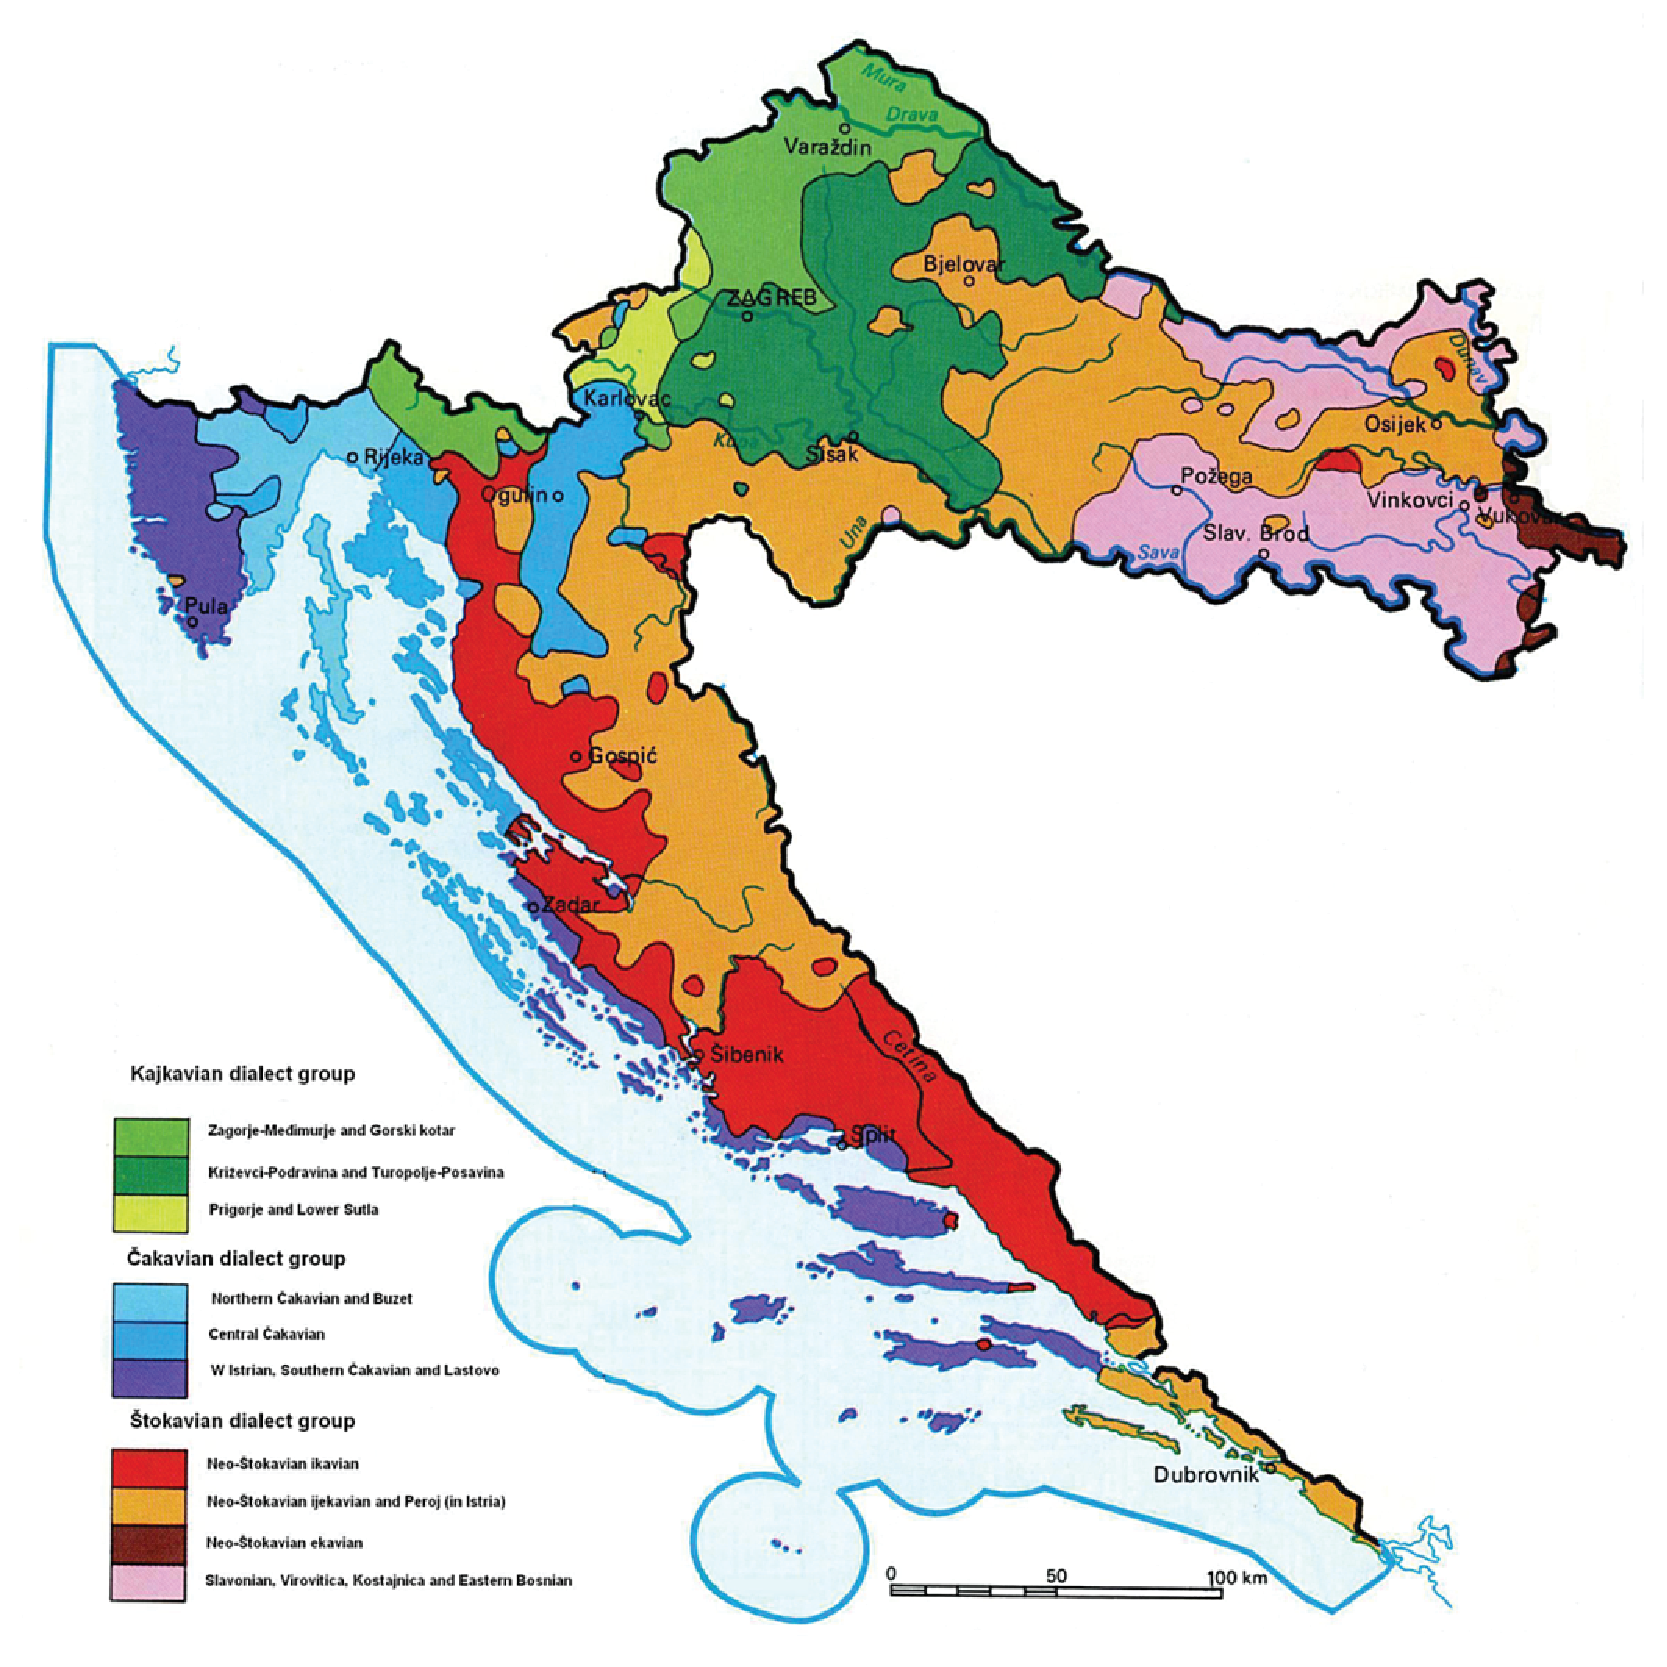
\includegraphics[width=\textwidth]{../_media/croatian/map-dialects}
  \caption{Map of Croatian dialects in the Republic of Croatia}
  \label{fig:dijalekti_en}
  \colorrule{grey3}{\textwidth}{1.5pt}
\end{figure*}


\subsection{Standardisation of Croatian language}

The millennial history of the Croatian language is attested to by texts written as early as the end of the 10th or the beginning of the 11th century, the period in which the three Croatian dialects (Čakavian, Štokavian, Kajkavian) began to form. All three Croatian dialects played an important part in the formation of the Croatian literary language (various dialectal stylizations) and the moulding of the Croatian linguistic culture that led to the Croatian standard language with a Štokavian foundation.

\boxtext{Did you know that the etymology of the\\ word „cravatte“ ('tie') comes from „Croatian“ and from French in 17th century it spread\\ to other languages?}

The first clear trends towards the shaping of the Croatian standard language became apparent in the 17th century, when the majority of the Croatian ethnic community - especially after the grammar and other works of Bartol Kašić (1575 - 1650) and a flourishing of Renaissance and Baroque literature from Štokavian Dubrovnik - recognised the linguistic structure of the Štokavian dialect (firstly with the ikavian \emph{jat} reflex, but later with the jekavian reflex) as the best starting point for the construction of a supra-regional Croatian literary language. Despite the choice of one linguistic structure in the construction of their standard language, the Croats did not dismiss the achievements of the centuries-old linguistic cultures of various dialectal stylisations within the Croatian literary language (Kajkavian, Štokavian, Čakavian, hybrid) that had marked its history within the Croatian ethnic community. Although the standardisation of the language of the Croats based upon the Štokavian dialect began very early, national linguistic unity was only achieved during the time of the Illyrian national revival (starting in 1835), when smaller groups of Croats who had until then expressed themselves in the Kajkavian idiom also accepted the Štokavian Croatian standard language. Throughout most of the 20th century, the Croatian standard language developed in various South Slavic state units under various names, and was presented as a variant of the so-called Croato-Serbian (Serbo-Croatian) language. This was abandoned during the socio-political changes of 1990.

Different stylisations of the Croatian language were shaped in diaspora long in the past (e.\,g.,~Burgenland Croatian, Molise Croatian). Croatian written culture is marked by the use of three alphabets (Glagolitic, Cyrillic, Latin), and the Latin script has been the foremost of the three among the Croats since the 16th century. Its usage was neither normed nor systematised until 1835, when Ljudevit Gaj gave the Croatian Latin alphabet its modern-day form.

\subsection{Characteristics of the Croatian language}

\subsubsection{Phonetics, phonology, morphonology}

The phoneme inventory of the Croatian standard language consists of 5 vowels (\emph{a, e, i, o, u}) and 25 consonants (\emph{m, v, n, l, r, j, nj, lj, p, b, f, s, z, c, t, d, ć, đ, š, ž, č, dž, h, k, g}).  The acoustic and articulatory characteristics of the vowels do not change depending on their placement (regardless whether in a short, long, accented or unaccented syllable). In addition to these 5 vowels, there also exist the syllabic \emph{r} (\emph{crn} ‘black’) and the diphthong \emph{ie}, which is marked in writing as \emph{je}/\emph{ije} (\emph{djelo, odijelo}).

The prosodic system consists of 4 accents (two long accents with a descending and ascending tone and two short accents with descending and ascending tone) and unaccented post-accentual lengths. The accentual system of the Croatian standard language is neo-štokavian, although it exists today with many differentiations from the prosodic models codified in the second half of the 19th century. Accent location is not fixed to a specific syllable, but the distribution of accents does have some limitations (e.\,g.,~the last syllable of a multi-syllable word cannot in principle be accentuated, descending accents are realised only in the initial syllables of non-compound words). These rules are broken in everyday speech, especially in large urban centres that are not located in Neo-štokavian regions (e.\,g.,~\emph{kontinuitêt  / kontinuìtēt}). Accent and length can have a differentiating role as they occasionally differentiate the meaning of lexemes or their wordforms, e.\,g.,~\emph{grȁd}  (= ‘hail’) : \emph{grâd} (= ‘town, city’), \emph{žènē}  (Gen. sing.) : \emph{žène}  (Nom.plur.). 

In Croatian some words do not have their own accent (clitic), but in an accentual unit proclitics can carry an accent passed over from an accented word with a descending accent in the initial syllable (\emph{grâd} : \emph{ȕ grād}), while enclitics cannot do this. The transfer of an accent onto a proclitic is becoming ever more rare in everyday speech, especially in urban centres not located in neo-Štokavian regions.

The Croatian standard language is characterised by a number of phonologically (Nom. sing. \emph{sla\textbf{d}ak} : Gen. sing. \emph{sla\textbf{t}koga}, Nom. sing. \emph{dio} : Gen. sing. \emph{dijela}) and morphonologically conditioned alternations (Nom. sing. \emph{maj\textbf{k}a} : Dat. sing. \emph{maj\textbf{c}i}, Nom. sing. \emph{juna\textbf{k}} : Voc. sing. \emph{juna\textbf{č}e}).

Regional implementation of the Croatian standard language is often influenced in speech by dialects located in a given region, e.\,g.,~in the Čakavian Kvarner region the prevalence of the plosive \emph{t'} in place of the voiceless africate \emph{ć}, or in the northwestern (Kajkavian) region, the non-differentiation of \emph{č} - \emph{ć} and \emph{đ} - \emph{dž}. 

\subsubsection{Morphology}

The Croatian standard language differentiates between ten parts of speech, of which five inflect (nouns, adjectives, numbers, pronouns, verbs) and four do not inflect (prepositions, conjunctions, particles, exclamations), while adverbs inflect only in comparation.

Grammatical categories that characterise the majority of declinable words are gender (three values: masculine, neuter, feminine), number (two values: singular, plural), case (seven values: nominative, genitive, dative, accusative, vocative, locative, instrumental). Some declinable words have special categories (e.\,g.,~definiteness is marked on adjectives with a full set of inflectional endings; animacy is marked by ending in masculine nouns and adjectives; nouns can be concrete, material, categorial or collective etc.). Words that are conjugated (verbs) are characterised by the categories of: manner (four values: indicative, imperative, conditional, optative), person (three values: 1st, 2nd, 3rd), number (two values: singular, plural), voice (two values: active, passive), tense (seven values: present, aorist, imperfect, perfect, pluperfect, future 1, future 2). The verbs \emph{biti} (‘to be’) and \emph{htjeti} (‘to will’) are auxiliary in Croatian. Verbs also have complicated aspectual system (imperfective and perfective with additional subvalues such as inchoativity, iterativity etc.) and they also encode the feature of transitivity. Adjectives and adverbs can take comparative forms (three values: positive, comparative, superlative).

Declension has two main types: noun declension (nouns and indefinite form of adjectives) and pronoun-adjective declension (pronouns, definite form of adjectives, numbers). Each noun gender has its own declension (a-type for masculine and neuter gender, e-type for feminine gender), and there is a special i-type (feminine gender nouns).

\begin{figure*}[htb]
\centering
	\begin{tabular}{|l|l|l|}
  \hline
  \textbf{Noun declension} & \textbf{N and G singular} & \textbf{N plural} \\ 
  \hline \hline
  a-type masculine    & \emph{opis, opis\textbf{a}}     &  \emph{opis\textbf{i}} \\ 
  \hline
  a-type neuter   & \emph{sunce, sunc\textbf{a}}     &  \emph{sunc\textbf{a}} \\ 
  \hline
  e-type feminine   & \emph{žen\textbf{a}, žen\textbf{e}}     &  \emph{žen\textbf{e}} \\
  \hline
  i-type feminine   & \emph{noć, noć\textbf{i}}     &  \emph{noć\textbf{i}} \\
  \hline
  \end{tabular}
  \caption{Noun declension in the Croatian language}
  \label{fig:imenicka_en}
\end{figure*}

Suffixes for adjective-pronoun declension are shown in this table:

\begin{figure*}[htb]
\centering
    \begin{tabular}{|l|l|l|l|}
        \hline
        \textbf{Case} & \textbf{Masculine}        & \textbf{Neuter}       & \textbf{Feminine} \\ \hline
		\multicolumn{4}{|c|}{\textbf{Singular}} \\ \hline
        N     & -i                & -o -e             & -a\\ 
        G     & -og(a) -eg(a)     & -og(a) -eg(a)     & -e\\ 
        D     & -om(u/e) -em(u/e) & -om(u/e) -em(u/e) & -oj\\ 
        A     & = N / = G         & = N               & -u\\ 
        V     & = N               & = N               & = N\\ 
        L     & -om(u/e) -em(u/e) & -om(u/e) -em(u/e) & = D\\ 
        I     & -im               & -im               & -om\\ \hline
		\multicolumn{4}{|c|}{\textbf{Plural}} \\ \hline
		N     & -i        & -a         & -e\\ 
        G     & -ih       & -ih        & -ih\\ 
        D     & -im(a)    & -im(a)     & -im(a)\\ 
        A     & -e        & = N        & = N\\ 
        V     & = N       & = N        & = N\\ 
        L     & = D       & = D        & = D\\ 
        I     & = D       & = D        & = D\\
        \hline
   \end{tabular}
  \caption{Adjective-pronoun declension in the Croatian language}
  \label{fig:zamjenicka_en}
\end{figure*}

Words in Croatian are formed by derivation and compounding. There are a few different methods of formation: suffix formation (\emph{star-ac}), prefix-suffix formation (\emph{do-život-an}), compound non-suffix formation (\emph{plači-drug}), compound suffix formation (\emph{vanjsk-o-politički}), coalescence (\emph{uz-brdo}), formation through compound abbreviations (\emph{Varteks}) and conversion (\emph{mlada}). Suffix formation is the most common. 

\subsubsection{Vocabulary, phraseology, terminology}

The foundational lexical layer of the Croatian standard language, aside from proto-Slavonic lexical heritage, consists of Štokavian vocabulary with an admixture of vocabulary from other Croatian dialects or vocabulary inherited from the literary language of various dialectal stylisations from older periods (e.\,g.,~from Kajkavian, \emph{kukac}, \emph{hlače}, \emph{rječnik}, or Čakavian, \emph{spužva}). Aside from this, the Croatian language as a whole bears witness to direct and indirect contact with other cultures. The Croatian language stands out among the remaining South Slavic languages in significant lexical influence received from Romance languages (substrate traces of the Dalmatic language, e.\,g.,~\emph{jarbol}, \emph{tunj}).  Italian significantly influenced the coastal regions of Croatia (especially the parts formerly under Venetian control), while German and, to an extent, Hungarian influenced the continental part. 

The Church Slavonic literary language left traces in older historical periods of the Croatian language, and so it did not present a great influence during the time in which the standard language was being shaped. Russian did not leave as a deep mark on Croatian as it did on the neighbouring Serbian standard language. The influence of the vocabulary of classical languages (Latin and Greek) is omnipresent in Croatian culture, especially in intellectual vocabulary, and scientific terminology. During the middle-Croatian period (16th - 18th century), Turkish loan words intensively entered the Croatian language, especially words related to everyday life. It is interesting to note that Burgenland Croatian, due to early migrations, does not have any Turkish loanwords, not even those that are in standard Croatian no longer perceived as foreign words (e.\,g.,~\emph{bubreg}, \emph{čizma}, \emph{jastuk}, etc.). In contrast to those loan-words, Burgenland Croatian uses older Croatian words of common Slavic origin and is therefore very important for the history of Croatian lexical inventory. German and French once had an influence on Croatian vocabulary, and in the second half of the 20th century, the influence of English has been ever stronger. The Czech language, although not in direct contact, has had a strong influence on Croatian vocabulary in several episodes, especially in the 19th century in professional terminology enriched by Bogoslav Šulek (e.\,g.,~\emph{časopis}, \emph{kisik}, \emph{dušik}, \emph{vodik}). During the period of Yugoslavia, Croatian was influenced by the Serbian language, especially because of common federal state administration. Purist tendencies in vocabulary came about occasionally from the 16th to the 20th century (e.\,g.,~Zoranić, Ritter Vitezović, Reljković, the period from 1941 - 1945).

Continuity from ancient times to the modern-day Croatian standard language and the participation of three dialects in the construction of the Croatian standard language can be seen in its well-developed and rich phraseology (e.g., in his 16th century stylised texts, Marulić uses the phraseme \emph{zgubiti glas} = ‘to be ashamed, to lose face’, while Zoranić uses the phraseme \emph{u magnutje oka} = ‘immediately’, which are nearly the same as the phrasemes \emph{izgubiti glas} and \emph{u trenu oka} in the Štokavian-structured standard language).

Terminology in specific professional fields began to develop as early as the 16th century, confirmed by the numerous Croatian (mostly multi-lingual) dictionaries compiled from the 16th to the 20th century. In the 19th century, German and Czech had especially strong influence on Croatian terminology, and English has today assumed this role.

\subsubsection{Syntax}

The Croatian language belongs to a group of languages characterised by an SVO syntactic structure (\emph{Marija voli Ivana}) and relatively free word order (numerous permutations of constituents are possible with some limitations, such as clitic placement). As concerns the information structure of sentences, it is a basic rule for structuring stylistically unmarked discourse that the first place is taken by the \emph{theme} (old information), which is followed by the \emph{rheme} (comment, new information).

The subject of a sentence does not have to be explicitly stated, and its omission is desirable insofar as it is repeated a number of times within a narrow context. Double-negation is required (\emph{Nitko ga nije volio}). The agreement of components in gender, number and case is typical of Croatian sentence structure.

There are seven cases in the Croatian standard language, and case forms are combined with prepositions (obligatory for the locative case). An important characteristic of Croatian verbs is their aspect while verb forms also express both tense and modal meaning. Sentence organisation can be both coordinated and subordinated (with the aid of conjunctions or without them). A relatively new occurrence in the modern language is the ever$-$less common use of the Slavonic genitive (\emph{Nije volio vina}), genitive expressions of possession are avoided in favour of possesive adjectives (\emph{majčina kuća} instead of \emph{kuća majke}), and the use of preterite tenses is reduced (imperfect, aorist and pluperfect). In modern Croatian passive constructions are rarer than in the older Croatian language.

\subsubsection{Orthography}

Although the history of Croatian culture has been marked by the use of three scripts (Glagolitic, Cyrillic and Latin script), the Latin script has been the dominant script used by Croats since the 16th century. The Croatian Latin alphabet was not fully standardized until 1835, when Ljudevit Gaj gave it its current-day form. It is composed of 30 characters, of which three are double characters (\emph{dž, lj, nj}), and the rest are single characters, of which five have diacritics (\emph{č, ć, đ, š, ž}). In academic circles, especially in the printing of texts from Croatian written heritage, the dual-characters \emph{dž}, \emph{lj} and \emph{nj}, are replaced by \emph{ģ}, \emph{ļ} and \emph{ń} respectively. The characters \emph{q, x, y, w} do not exist in the Croatian alphabet originally, although they are being used for writing foreign names.

\begin{figure*}[htb]
\centering
	\begin{tabular} {|c|c|c|c|c|c|c|c|c|c|c|c|c|c|c|}
        \hline
        \multicolumn{15}{|c|}{\textbf{Capital letters}} \\ \hline
        A & B  & C & Č & Ć  & D & DŽ & Đ & E & F & G & H & I & J & K \\ \hline
        L & LJ & M & N & NJ & O & P  & R & S & Š & T & U & V & Z & Ž \\ \hline
        \multicolumn{15}{|c|}{\textbf{Lowercase letters}} \\ \hline
        a & b  & c & č & ć  & d & dž & đ & e & f & g & h & i & j & k \\ \hline
        l & lj & m & n & nj & o & p  & r & s & š & t & u & v & z & ž \\
        \hline
   \end{tabular}
  \caption{The Croatian Latin alphabet }
  \label{fig:abeceda_en}
\end{figure*}

Croatian orthography is phonological-morphonological, since it presents a confluence of two orthographic principles: dominant phonological (e.\,g.,~the marking of assimilation) and subordinate morphonological (e.\,g.,~\emph{podcrtati}). Interword separation is logical, and not grammatical (as it once was). It is typical of Croatian orthography that the writing of foreign names is not adjusted to their pronunciation or the graphic inventory of the Croatian alphabet (e.\,g.,~\emph{John}, not \emph{Džon}, or \emph{Washington}, not \emph{Vašington}).

\subsubsection{Onomastics}

Croatian names represent important linguistic monuments of the linguistic, cultural and social heritage of the people who created them. Thus, both personal names (anthroponyms) and place names (toponyms) are an important segment of Croatian linguistic culture. The territory of present-day Croatia, roughly bound by the river Drava in the North, the river Danube  in the East and the Adriatic Sea in the South, is very picturesquely reflected in its complex stratification of geographical names. The complex stratification of Croatian toponymy reflects centuries of coexistence of the various ethnic groups that have settled on the Eastern coast of the Adriatic and its hinterland throughout history. Centuries of linguistic interpenetration and the merging of various cultural traditions have left an indelible imprint on Croatian toponymy. Furthermore, place names attestations are frequently the oldest witnesses to the oldest changes in the Croatian language itself. 

\boxtext{Did you know that Croats were the first Slavic nation to bear family names since 12th century?}

Since Croatian developed across religious (pre-christian and christian), cultural and civilisational borders, traces of both East and West have been left on Croatian names. With regards to personal names, Croatians were the first Slavic nation to bear family names (since the 12th century) along the Adriatic coast due to direct Romance cultural influence. The oldest layer of Croatian names is founded upon proto-Slavic name forms that are following common Indo-European name formation patterns. The patronymics form the basis for the largest part of inventory of family names but, unlike in Russian, they are not productive anymore and remain unchanged as frozen family names that are incorporated in inflectional system as nouns. In contrast to the Croatian toponomastic system, where we found almost no Turkish influence, many Croatian family names were formed upon Turkish loan-words with Croatian suffixes, since most family names in Croatia were created after the Council of Trent in the 16th century, at the time when a large portion of Croatian lands was under Turkish rule.

\subsection{The relationship between the Croatian standard language and other Štokavian-structured languages}

The four national languages, Croatian, Serbian, and recently Bosnian and Montenegrin, all share Štokavian structural basis, however the traditions and superstructures of these languages are fairly different. What is specific to Croatian linguistic history and culture among other the South Slavic languages is the relationship between its three dialects (Kajkavian, Čakavian, Štokavian), which continually enriches the Štokavian-structured Croatian standard language. Because of different starting points (the non-existence of a basic, common standard) and traditions in language cultivation and standardisation, the disunity of neo-Štokavian structure and differences in linguistic superstructure, one monolithic standard language was never formed during the existence of the Yugoslavian states, although there were serveral attempts of political imposition of the common name (\emph{Serbo-Croato-Slovenian} during the Kingdom of Yugoslavia; \emph{Serbo-Croatian} or \emph{Croato-Serbian}, \emph{Croatian} or \emph{Serbian} during the communist Yugoslavia). During the Second World War and few year later all official documents in Yugoslavia were published in four official languages (Croatian, Macedonian, Serbian, Slovenian), but soon a lot of political effort was put again into convergence of Croatian and Serbian. Despite all attempts to recognise the official existence of Croatian as a language on its own, the forcing of unified terminology, vocabulary, orthography and other linguistic norms in Yugoslavia, led to the official recognition of one standard language (\emph{Serbo-Croatian}) with two variants (\emph{eastern} or \emph{Serbian} and \emph{western} or \emph{Croatian}). The reaction from Croatia came in the form of \emph{Declaration on the Position of the Croatian Language} that openly advocated the recognition of the independent Croatian language and was unanimously signed in 1967 by leading scientific, cultural and educational institutions as well as leading intellectuals throughout Croatia who took a great risk with such an open political move in communist times.

In the past 20 years, the four Štokavian-structured standard languages have developed autonomously as national standard languages in naturally diverging way, and no agreement or coordination exists concerning their norming, which has increased differences between them.

\subsection{Linguistic cultivation in Croatia}

The Croatian Language Council was founded by a decision of the Ministry of Science, Education and Sport taken on 14th April 2005. Its basic task is the systematic and scientific care of the Croatian standard language. The specific tasks of the Council are:

\begin{itemize}
\item to tend to the Croatian standard language;
\item to discuss current dilemmas and open issues in the Croatian standard language;
\item to warn of cases of infractions of the constitutional decree on the position of Croatian as the official language of the Republic of Croatia;
\item to promote the culture of the Croatian standard language in written and oral communication;
\item to tend to the status and role of the Croatian standard language in light of Croatia’s integration into the European Union;
\item to make decisions on further standardisation processes of the Croatian standard language;
\item to take care of language issues and set principles for the orthographic standardization.
\end{itemize}

The Croatian Language Council meets regularly and draws conclusions after thorough debate. The Institute of Croatian Language and Linguistics hosts the Council, provides technical and administrative support as well as linguistic expertise when necessary.

The Institute of Croatian Language and Linguistics \cite{str7} is the central Croatian institution for the research of the Croatian language, and one department of the Institute (the Croatian Standard Language Department) is dedicated to the description of the Croatian standard language, with special attention paid to linguistic culture (e.\,g.,~work on offering linguistic advice to the public and the writing of language handbooks). Advice on proper language usage and linguistic expertise are permanent duties of the Institute. Advices are given by phone, e mail and in written form. Furthermore, the answers to the most frequently asked questions are available on the Language Advice Portal \cite{str8} on the Institute web site.

\boxtext{The basic task of the Croatian Language Council is the systematic and scientific care of the Croatian standard language.}

The Institute’s STRUNA project \cite{str9},  which develops the Croatian professional terminology, deserves a special mention. The goal of this project is to establish a system of coordinating terminological work in all professional fields in Croatia, and in doing so contribute to the improvement of the quality and effectiveness of higher education and scientific research work through the creation of unified and verified terminology that can be used by experts in all fields, as well as by interested participants from the general public. The establishment of a research terminology network and scientific cooperation between institutions that deal in various aspects of terminological work is also planned.

\boxtext{Today English loan words are common\\ in the informal language but much less so in\\ the formal or written language.}

Besides this, other Croatian scientific institutions (several universities with their departments of Croatian language and literature) and cultural institutions (such as \emph{Matica hrvatska}) also take part in the care of the Croatian language. Public media, such as state radio-television and some newspaper publishers, have well-developed proofreading services for the Croatian standard language and pay special attention to the quality of language they use in their public text production.

\subsection{Language in education}

Croatian language is official in all primary and secondary schools, except in regions with national minority residents. However, it is not defined as obligatory for the use at universities. There is a pronounced tendency in Croatia, especially in so-called “hard sciences” to teach in the English language. There were agreeable opinions that it could be functional and useful, but also harmful and unacceptable not to teach in the Croatian language at universities. It would have devastating effects for the development of the Croatian scientific terminology and occupational phraseology. Therefore “The Croatian Language Council” advised the Ministry to legally define the language usage at higher education.

In primary and secondary schools, Croatian language and literature is taught as a subject, and takes up considerable space in the curriculum. As part of this subject, Croatian grammar, vocabulary and literature is studied, and written and verbal expression in Croatian is developed. The PISA test, which tests the skills of pupils at the global level, has been executed in Croatia since 2006, and the first results of testing showed that Croatian 15-year-olds took 26th place of world countries, placed ahead of ten European Union member states and the United States of America.

Besides Croatian, in primary and secondary education it is obligatory to study at least one foreign language from the fourth grade. However, English language (only rarely French or German) is often taught already in kindergartens. English language is usually the first foreign language in primary education. The most widespread second foreign language is German, then Italian and French. In secondary education Russian and Spanish are occasionally taught as second or third foreign languages. Latin and Old Greek are taught in all classics-program schools that start from the fifth grade of primary school. Furthermore, Latin language is still obligatory in all humanistic secondary schools. In a Jewish minority school (which is open to general public), it is also possible to study Hebrew. Education on minority languages, from the kindergarten level to secondary education, is available and financed by the Croatian government for the Serbian, Czech, Hungarian and Italian minority.

\subsection{International aspects}

The use of the Croatian standard language in countries in the region is regulated by the laws of these countries. The status of the Croatian standard language as one of the official languages of neighbouring Bosnia and Herzegovina is especially important, and so Croatian institutions pay special attention to cooperation with scientific and cultural institutions of the Croatian nation in Bosnia and Herzegovina. The Republic of Croatia’s cultural institutions establish cooperation with many Croatian diasporic institutions throughout the world. 

\boxtext{When Croatia join the European Union in\\ 2013, the Croatian language will become the 24th official language of the EU.}

Lectures of Croatian language are organised in schools abroad for the children of Croatian citizens who reside either temporarily or permanently in other countries. The Croatian language is taught at many foreign institutions and Slavic studies centres (there are 36 official exchange instructorships for the Croatian language and literature as well as 2 centres for Croatian studies in Australia and Canada in the jurisdiction of and financed by the Ministry of Science, Education and Sport of the Republic of Croatia). A number of centres for the study of Croatian as a second or foreign language operate in Croatia, the best-known of which is \emph{Croaticum} \cite{str10}. 

\subsection{Croatian in the Internet}

According to the statistical information of the Croatian Bureau of Statistics, the use of information and communications technology in enterprises and households looks as follows in terms of percentages:

\begin{figure*}[htb]
\centering
    \begin{tabular}{|c|c|c|c|}
        \hline
      \multicolumn{4}{|c|}{\textbf{Usage of information and communication technologies(ICT) in enterprises(\%)}} \\ \hline
        ~                                              & 2008 & 2009 & 2010 \\ \hline
        \emph{Computer usage}                        & 98   & 98   & 97   \\ \hline
        \emph{Internet access}                       & 97   & 95   & 95   \\ \hline
        \emph{Web site}                            & 64   & 57   & 61   \\ \hline
        \emph{Usage of financial and banking services} & 84   & 84   & 85   \\ \hline
        \emph{E-government usage}                 & 56   & 61   & 63   \\
        \hline
   \end{tabular}
  \caption{ICT in enterprises}
  \label{fig:IST_pod_en}
\end{figure*}

\begin{figure*}[htb]
\centering
	\begin{tabular}{|c|c|c|c|}
        \hline
      \multicolumn{4}{|c|}{\textbf{Households equipped with information and communication technologies(ICT)(\%)}} \\ \hline
        ~                                              & 2008 & 2009 & 2010 \\ \hline
        \emph{Personal computer}   & 53   & 55   & 60   \\ \hline
        \emph{Internet access} & 45   & 50   & 57   \\ \hline
        \emph{Mobile phone}   & 81   & 82   & -    \\
        \hline
   \end{tabular}
  \caption{ICT in households}
  \label{fig:IST_kuc_en}
\end{figure*}

The most-visited Croatian websites are: net.hr (a news, sports, entertainment and events portal), \emph{index.hr} (general web portal, info, services, news, sports, entertainment, automotive, gastronomy), \emph{jutarnji.hr} (the website of the daily newspaper “Jutarnji list”), \emph{24sata.hr} (website of the daily newspaper “24 sata”), tportal.hr (newsportal of HT, Croatian Telecomm), \emph{njuskalo.hr} (“Njuškalo” advertisments portal), \emph{vecernji.hr} (website of the daily newspaper “Večernji list”), \emph{forum.hr} (the largest Croatian web forum, discussing society, culture, entertainment, etc.). Seven daily Croatian newspapers publish their articles on their own dedicated portals in addition to their paper versions.

\boxtext{The growing importance of the Internet is important for Language Technologies.}

The Institute of Croatian Language and Linguistics maintains the web page about the Croatian that features the comprehensive list of mono- and multilingual dictionaries, grammars and orthographies. At the Faculty of Humanities and Social Sciences a similar web page is maintained \cite{str11}. At the same Faculty a portal on Croatian Language Technologies \cite{str12} is maintained since 1999.

The Croatian-language Wikipedia was founded in 2003 and has 108,528 \footnote{Recorded on 2012-05-24} articles, being the 30rd Wikipedia by number of official articles.

Access to resources in Croatian has been made easier in recent times by Croatian institutions and organisations undergoing the digitalisation process (including significantly projects supported by Ministry of Science, Education and Sports and Ministy of Culture for digitising Croatian cultural heritage) which has increased the visibility of the Croatian language among internet sources.
\end{multicols}

\clearpage

\ssection[Language Technology Support for Croatian]{Language Technology Support for Croatian}

\begin{multicols}{2}
Language technologies are used to develop software systems designed to handle human language and are therefore often called “human language technologies”. Human language comes in spoken and written forms. While speech is the oldest and in terms of human evolution the most natural form of language communication, complex information and most human knowledge is stored and transmitted through the written word. Speech and text technologies process or produce these different forms of language, using dictionaries, rules of grammar, and semantics. This means that language technology (LT) links language to various forms of knowledge, independently of the media (speech or text) in which it is expressed. Figure ~\ref{fig:ltincontext_en} illustrates the LT landscape.

\begin{figure*}[htb]
  \colorrule{grey3}{\textwidth}{1.5pt}
  \center
  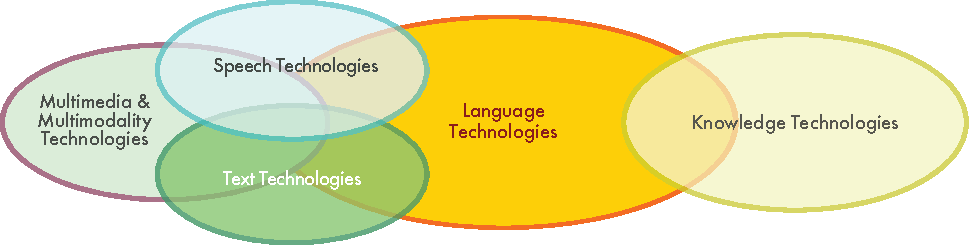
\includegraphics[width=\textwidth]{../_media/english/language_technologies}
  \caption{Language technologies}
  \refstepcounter{refs_en}
  \label{fig:ltincontext_en}
  \colorrule{grey3}{\textwidth}{1.5pt}
\end{figure*}

When we communicate, we combine language with other modes of communication and information media—for example speaking can involve gestures and facial expressions. Digital texts link to pictures and sounds. Movies may contain language in spoken and written form. In other words, speech and text technologies overlap and interact with other multimodal communication and multimedia technologies.

In this section, we will discuss the main application areas of language technology, i.e., language checking, web search, speech interaction, and machine translation. These applications and basic technologies include:

\begin{itemize}
\item spelling correction
\item authoring support
\item computer-assisted language learning
\item information retrieval
\item information extraction
\item text summarisation
\item question answering
\item speech recognition
\item speech synthesis
\end{itemize}

Language technology is an established area of research with an extensive set of introductory literature. The interested reader is referred to the following references: \cite{boo6, boo7, boo8, str37, boo9}.

Before discussing the above application areas, we will briefly describe the architecture of a typical LT system.

\subsection{Application Architectures}

Software applications for language processing typically consist of several components that mirror different aspects of language. While such applications tend to be very complex, figure~\ref{fig:textprocessingarch_en} shows a highly simplified architecture of a typical text processing system. The first three modules handle the structure and meaning of the text input:

\begin{enumerate}
\item Pre-processing: cleans the data, analyses or removes formatting, detects the input languages, and so on.
\item Grammatical analysis: finds the verb, its objects, modifiers and other sentence elements; detects the sentence structure.
\item Semantic analysis: performs disambiguation (i.\,e., computes the appropriate meaning of words in a given context); resolves anaphora (i.\,e., which pronouns refer to which nouns in the sentence); represents the meaning of the sentence in a machine-readable way.
\end{enumerate}

\begin{figure*}[b]
  \colorrule{grey3}{\textwidth}{1.5pt}
  \center
  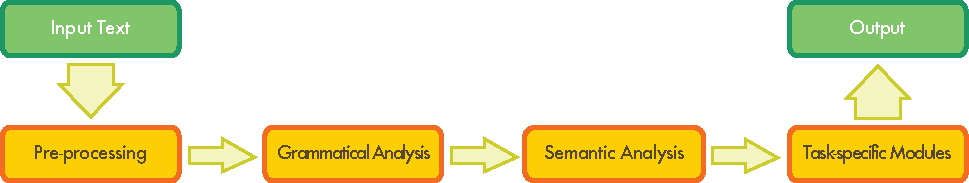
\includegraphics[width=\textwidth]{../_media/english/text_processing_app_architecture}
  \caption{A typical text processing architecture}
  \refstepcounter{refs_en}
  \label{fig:textprocessingarch_en}
  \colorrule{grey3}{\textwidth}{1.5pt}
\end{figure*}

After analysing the text, task-specific modules can perform other operations, such as automatic summarisation and database look-ups.

In the remainder of this section, we firstly introduce the core application areas for language technology, and follow this with a brief overview of the state of LT research and education today, and a description of past and present research programmes. Finally, we present an expert estimate of core LT tools and resources for Croatian in terms of various dimensions such as availability, maturity and quality. The general situation of LT for the Croatian language is summarised in figure~\ref{fig:resursi_en} (p.~\pageref{fig:resursi_en}) at the end of this chapter. This table lists all tools and resources that are \textbf{boldfaced} in the text. LT support for Croatian is also compared to other languages that are part of this series.

\subsection{Core application areas}

In this section, we focus on the most important LT tools and resources, and provide an overview of LT activities in Croatia.

\subsubsection{Language Checking}

\begin{figure*}[t]
  \colorrule{grey3}{\textwidth}{1.5pt}
  \center
  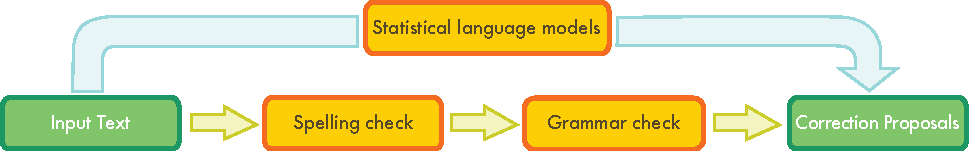
\includegraphics[width=\textwidth]{../_media/english/language_checking}
  \caption{Language checking (top:statistical; bottom:rule-based)}
  \refstepcounter{refs_en}
  \label{fig:langcheckingaarch_en}
  \colorrule{grey3}{\textwidth}{1.5pt}
\end{figure*}

Anyone who has used a word processor such as Microsoft Word knows that it has a spell checker that highlights spelling mistakes and proposes corrections. The first spelling correction programs compared a list of extracted words against a dictionary of correctly spelled words. Today these programs are far more sophisticated. Using language-dependent algorithms for \textbf{grammatical analysis}, they detect errors related to morphology (e.\,g., plural formation) as well as syntax--related errors, such as a missing verb or a conflict of verb-subject agreement (e.\,g., \textit{she *write a letter}). However, most spell checkers will not find any errors in the following text \cite{art11}:

\begin{itemize}
\item[] I have a spelling checker,\\
  It came with my PC.\\
  It plane lee marks four my revue\\
  Miss steaks aye can knot sea.
\end{itemize}

Handling these kinds of errors usually requires an analysis of the context. For example: deciding if an Croatian noun should be written with capital first letter (female personal name) or not (common noun), as in:

\begin{itemize}
\item \textbf{Slatka je ova višnja.}.\\
  {[}This cherry is sweet.{]} 
\item \textbf{Slatka je ova Višnja.}.\\
  {[}This Cherry is sweet.{]}
\end{itemize}

This type of analysis either needs to draw on language-specific \textbf{grammars} laboriously coded into the software by experts, or on a statistical language model. In this case, a model calculates the probability of a particular word as it occurs in a specific position (e.\,g.,~between the words that precede and follow it). For example: \emph{jaz između} (‘gap between’) is much more probable word sequence than \emph{jaz generacija} (‘generation gap’). A statistical language model can be automatically created by using a large amount of (correct) language data, a \textbf{text corpus}. Most of these two approaches have been developed around data from English. Neither approach can transfer easily to Croatian because the language has a flexible word order and rich inflection that contribute abundantly to the data sparsness problem in such systems.

Language Checking is not limited to word processors; it is also used in “authoring support systems”, i.\,e., software environments in which manuals and other types of technical documentation for complex IT, healthcare, engineering and other products, are written. To offset customer complaints about incorrect use and damage claims resulting from poorly understood instructions, companies are increasingly focusing on the quality of technical documentation while targeting the international market (via translation or localisation) at the same time. Advances in natural language processing have led to the development of authoring support software, which helps the writer of technical documentation to use vocabulary and sentence structures that are consistent with industry rules and (corporate) terminology restrictions, but such systems are not yet available for Croatian.

\boxtext{Language checking is not limited to word processors but also applies to authoring systems.}

Although the research on computational models of inflectional morphology existed in 1980s the first industry-strength spelling checker for Croatian Hrvatski računalni pravopis has been published in 1996 \cite{boo2}. Soon after it was bought by Microsoft and today it represents the integral part of Croatian MS Office proofing tools and it is widely used. Other spelling checkers have also been developed by several private companies, but none of them has been so successful. An on-line Croatian Academic Spelling Checker (Hascheck) \cite{str13} exists from 1994. and it is still in use. An open source spelling checker for Croatian also exist, it can be used with OpenOffice on different operating systems and is based on Ispell/Aspell. These programs are based on the very large lexicon of correct wordforms which have two drawbacks: 1) strings that represent correct wordforms appearing in a wrong co text; 2) inability to distinguish between real spelling errors and wordforms which are correct, but which are unknown to the lexicon. Besides spell checkers and authoring support, Language Checking is also important in the field of computer-assisted language learning and is applied to automatically correct queries sent to Web Search engines, e.\,g.,~Google’s \textit{Did you mean…} suggestions. 

\subsubsection{Web Search}

Searching the Web, intranets or digital libraries is probably the most widely used yet largely underdeveloped language technology application today. The Google search engine, which started in 1998, now handles about 80\% of all search queries \cite{str14}. Since 2004, the verb \emph{guglati/googlati} and its derivatives \emph{(iz-/na-/pre-/pro-/u-)guglati/(iz-/na-/pre-/pro-/u-)googlati} is used in Croatian, even though it has not made its way into printed dictionaries (even more complex derivatives such as \emph{ugugljiv} ‘googlable’ are recorded). The Google search interface and results page display has not significantly changed since the first version. However, in the current version, Google offers spelling correction for misspelled words and incorporates basic semantic search capabilities that can improve search accuracy by analysing the meaning of terms in a search query context \cite{str15}. With the help of this algorithm it also started to cover some of the wordforms in which Croatian lexemes could appear in texts. Unlike the e.\,g.,~English nouns where only four wordforms are possible for a noun lexeme (\emph{hand, hand’s, hands, hands’}) in Croatian theoretically it can appear in 14 different wordforms, but they are represented on average with 10 different types (\emph{ruka, ruke, ruci, ruku, rukom, rukama}...). Google search engine can retrieve forms like \emph{ruka, ruke}, but \emph{ruci} is still not connected to lemma \emph{ruka}. There is a room for improvement when Google has to deal with inflectionally rich languages where lexemes appear in many different wordforms. The Google success story shows that a large volume of data and efficient indexing techniques can deliver satisfactory results using mainly statistical approach to language processing, but they also depend heavily on the language structure.

\boxtext{The next generation of search engines\\ will have to include much more sophisticated language technology.}

For more sophisticated information requests, it is essential to integrate deeper linguistic knowledge to facilitate text interpretation. Experiments using \textbf{lexical resources} such as machine-readable thesauri or ontological language resources (e.\,g., WordNet for English or Croatian Wordnet, CroWN for Croatian) have demonstrated improvements in finding pages using synonyms of the original search terms, such as \emph{nuklearna energija} and \emph{atomska energija} (nuclear energy and atomic energy) or even more loosely related terms. 

\begin{figure*}[t]
  \colorrule{grey3}{\textwidth}{1.5pt}
  \center
  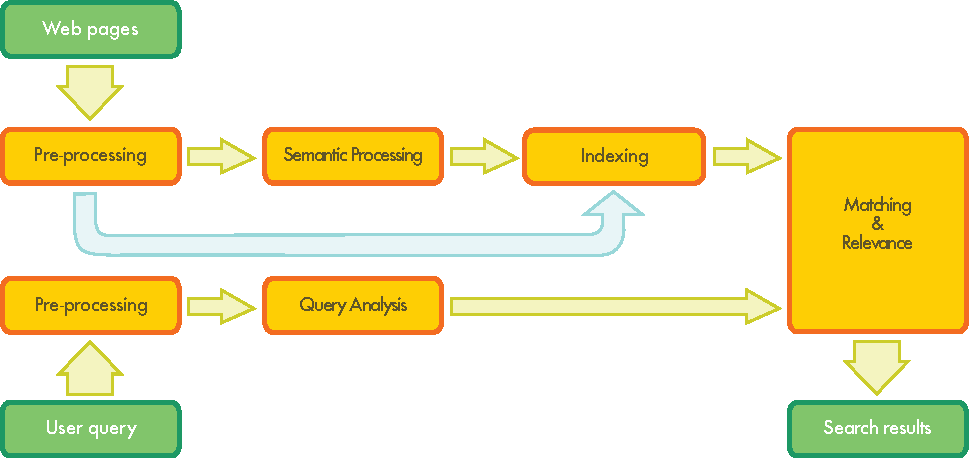
\includegraphics[width=\textwidth]{../_media/english/web_search_architecture}
  \caption{Web search}
  \refstepcounter{refs_en}
  \label{fig:websearcharch_en}
  \colorrule{grey3}{\textwidth}{1.5pt}
 \end{figure*}


The next generation of search engines will have to include much more sophisticated language technology, especially to deal with search queries consisting of a question or other sentence type rather than a list of keywords. For the query, \emph{Give me a list of all companies that were taken over by other companies in the last five years}, a syntactic as well as \textbf{semantic analysis} is required. The system also needs to provide an index to quickly retrieve relevant documents. A satisfactory answer will require syntactic parsing to analyse the grammatical structure of the sentence and determine that the user wants companies that have been acquired, rather than companies that have acquired other companies. For the expression \emph{last five years}, the system needs to determine the relevant range of years, taking into account the present year. The query then needs to be matched against a huge amount of unstructured data to find the pieces of information that are relevant to the user’s request. This process is called information retrieval, and involves searching and ranking relevant documents. To generate a list of companies, the system also needs to recognise a particular string of words in a document represents a company name, using a process called named entity recognition. A more demanding challenge is matching a query in one language with documents in another language. Cross-lingual information retrieval involves automatically translating the query into all possible source languages and then translating the results back into the user’s target language.

Now that data is increasingly found in non-textual formats, there is a need for services that deliver multimedia information retrieval by searching images, audio files and video data. In the case of audio and video files, a speech recognition module must convert the speech content into text (or into a phonetic representation) that can then be matched against a user query.

For inflectional languages like Croatian, it is important to be able to search for all the inflectional forms of a word at once, instead of having to enter each different form separately. This can be done with the aid of the Croatian Lemmatisation Server that has been developed at the Department of Linguistics, Faculty of Humanities and Social Sciences at the University of Zagreb and is freely accessible \cite{str16} providing an interface to the Croatian Morphological Lexicon, a comprehensive full wordforms database. It contains over 110,000 lexemes yielding over 4 million inflectional wordforms where each entry contains lemma, wordform and full MSD tag and it is MulText East \cite{str17} compliant.

In 2009 as a result of a joint Flemish-Croatian project CADIAL \cite{str18}, the governmental agency HIDRA enabled the public web access to all Croatian legislative documents using the inflectionally sensitive search engine \cite{str19}. This engine also enables cross-lingual document retrieval since all documents are indexed with EUROVOC descriptors thus allowing the usage of English EUROVOC descriptors in queries.

\subsubsection{Speech Interaction}

Speech interaction is one of many application areas that depend on speech technology, i.\,e., technologies for processing spoken language. Speech interaction technology is used to create interfaces that enable users to interact in spoken language instead of using a graphical display, keyboard and mouse.  Today, these voice user interfaces (VUI) are used for partially or fully automated telephone services provided by companies to customers, employees or partners. Business domains that rely heavily on VUIs include banking, supply chain, public transportation, and telecommunications. Other uses of speech interaction technology include interfaces to car navigation systems and the use of spoken language as an alternative to the graphical or touchscreen interfaces in smartphones.

Speech interaction technology comprises four technologies: 

\begin{enumerate}
\item Automatic \textbf{speech recognition} (ASR) determines which words are actually spoken in a given sequence of sounds uttered by a user.  
\item Natural language understanding analyses the syntactic structure of a user’s utterance and interprets it according to the system in question.
\item Dialogue management determines which action to take given the user input and system functionality.   
\item \textbf{Speech synthesis} (text-to-speech or TTS) transforms the system’s reply into sounds for the user.
\end{enumerate}

One of the major challenges of ASR systems is to accurately recognise the words a user utters. This means restricting the range of possible user utterances to a limited set of keywords, or manually creating language models that cover a large range of natural language utterances. Using machine learning techniques, language models can also be generated automatically from \textbf{speech corpora}, i.\,e., large collections of speech audio files and text transcriptions. Restricting utterances usually forces people to use the voice user interface in a rigid way and can damage user acceptance; but the creation, tuning and maintenance of rich language models will significantly increase costs. VUIs that employ language models and initially allow a user to express their intent more flexibly — prompted by a \textit{How may I help you?} greeting — tend to be automated and are better accepted.

Companies tend to use utterances pre-recorded by professional speakers for generating the output of the voice user interface. For static utterances where the wording does not depend on particular contexts of use or personal user data, this can deliver a rich user experience. But more dynamic content in an utterance may suffer from unnatural intonation because different parts of audio files have simply been strung together. Through optimisation, today’s TTS systems are getting better at producing natural-sounding dynamic utterances.

\boxtext{Speech interaction is the basis for creating interfaces that allow a user to interact with\\ spoken language instead of a graphical\\ display, keyboard and mouse.}

\begin{figure*}[t]
  \colorrule{grey3}{\textwidth}{1.5pt}
  \center
  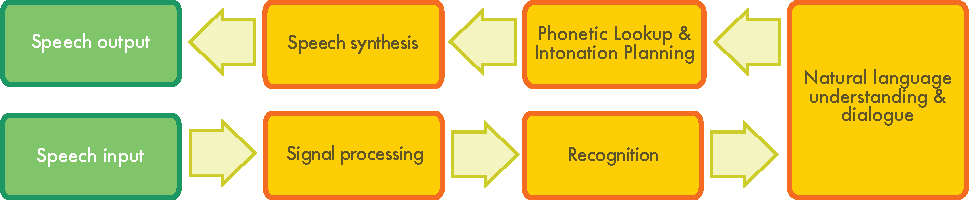
\includegraphics[width=\textwidth]{../_media/english/simple_speech-based_dialogue_architecture}
  \caption{Speech-based dialogue system}
  \refstepcounter{refs_en}
  \label{fig:dialoguearch_en}
  \colorrule{grey3}{\textwidth}{1.5pt}
\end{figure*}

Interfaces in speech interaction have been considerably standardised during the last decade in terms of their various technological components. There has also been strong market consolidation in speech recognition and speech synthesis. The national markets in the G20 countries (economically resilient countries with high populations) have been dominated by just five global players, with Nuance (USA) and Loquendo (Italy) being the most prominent players in Europe. In 2011, Nuance announced the acquisition of Loquendo, which represents a further step in market consolidation.

Although the Croatian diphone base was developed within the MBROLA \cite{str20} project in 1998 in which Department of Phonetics, Faculty of Humanities and Social Sciences, University of Zagreb participated, up to now, there has been no commercial application of Croatian TTS or ATS systems developed in Croatia. Research in this field has been conducted also at the Faculty of Electrical Engineering and Computing of the same university \cite{art1} as well as at the University of Rijeka where a strong group works on the development of resources and tools for speech processing of Croatian \cite{str2, str21, art3}]. 

Looking ahead, there will be significant changes, due to the spread of smartphones as a new platform for managing customer relationships, in addition to fixed telephones, the Internet and e-mail. This will also affect how speech interaction technology is used. In the long term, there will be fewer telephone-based VUIs, and spoken language apps will play a far more central role as a user-friendly input for smartphones. This will be largely driven by stepwise improvements in the accuracy of speaker-independent speech recognition via the speech dictation services already offered as centralised services to smartphone users.

\subsection{Machine Translation}

\begin{figure*}[htb]
  \colorrule{grey3}{\textwidth}{1.5pt}
  \center
  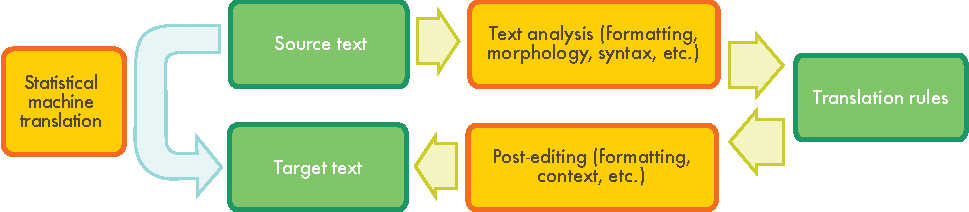
\includegraphics[width=\textwidth]{../_media/english/machine_translation}
  \caption{Machine translation (left:statistical; right:rule-based)}
  \refstepcounter{refs_en}
  \label{fig:mtarch_en}
  \colorrule{grey3}{\textwidth}{1.5pt}
\end{figure*}

The idea of using digital computers to translate natural languages can be traced back to 1946 and was followed by substantial funding for research during the 1950s and again in the 1980s. Yet \textbf{machine translation} (MT) still cannot meet its initial promise of across-the-board automated translation.
 
\boxtext{At its basic level, Machine Translation\\ simply substitutes words in one natural language\\ with words in another language.}

The most basic approach to machine translation is the automatic replacement of the words in a text written in one natural language with the equivalent words of another language. This can be useful in subject domains that have a very restricted, formulaic language such as weather reports. However, in order to produce a good translation of less restricted texts, larger text units (phrases, sentences, or even whole passages) need to be matched to their closest counterparts in the target language. The major difficulty is that human language is ambiguous. Ambiguity creates challenges on multiple levels, such as word sense disambiguation at the lexical level (a \emph{jaguar} is a brand of car or an animal) or the assignment of the prepositional phrases on the syntactic level, e.\,g.,~as in:

\begin{itemize}
\item Policajac je uočio čovjeka bez teleskopa.\\
  {[}The policeman spotted a man without a telescope.{]} 
\item Policajac je uočio čovjeka bez pištolja.\\
  {[}The policeman spotted a man without a pistol.{]}
\end{itemize}

One way to build an MT system is to use linguistic rules. For translations between closely related languages, a translation using direct substitution may be feasible in cases such as the above example. However, rule-based (or linguistic knowledge-driven) systems often analyse the input text and create an intermediary symbolic representation from which the target language text can be generated. The success of these methods is highly dependent on the availability of extensive lexicons with morphological, syntactic, and semantic information, and large sets of grammar rules carefully designed by skilled linguists. This is a very long and therefore costly process.

In the late 1980s when computational power increased and became cheaper, interest in statistical models for machine translation began to grow. Statistical models are derived from analysing bilingual text corpora, \textbf{parallel corpora}, such as the Europarl parallel corpus, which contains the proceedings of the European Parliament in 21 European languages or JRC Acquis parallel corpus in 22 European languages \cite{pro1}. Given enough data, statistical MT works well enough to derive an approximate meaning of a foreign language text by processing parallel versions and finding plausible patterns of words. Unlike knowledge-driven systems, however, statistical (or datadriven) MT systems often generate ungrammatical output. Data-driven MT is advantageous because less human effort is required, and it can also cover special particularities of the language (e.\,g., idiomatic expressions) that are often ignored in knowledge-driven systems. Regarding the European languages, acceptable translations can be obtained for English and the Romance languages, but the quality is downgraded substantially for Germanic, Slavic, Finno-Ugric and Baltic languages \cite{pro2}.

\boxtext{Machine Translation is particularly\\ challenging for Slavic languages because of\\ their free word order, inflectional richness and long distance dependencies.}

The strengths and weaknesses of knowledge-driven and data-driven machine translation tend to be complementary, so that nowadays researchers focus on hybrid approaches that combine both methodologies. One such approach uses both knowledge-driven and data-driven systems, together with a selection module that decides on the best output for each sentence. However, results for sentences longer than, say, 12 words, will often be far from perfect. A more effective solution is to combine the best parts of each sentence from multiple outputs; this can be fairly complex, as corresponding parts of multiple alternatives are not always obvious and need to be aligned. 

For Croatian, MT is particularly challenging. The free word order and extensive inflection is a challenge for generating words with proper endings that mark grammatical categories of gender, case, number, mood, tense, etc. Also the required agreement in all these categories between e.\,g.,~attributes and their nouns or only in number and gender for subject and predicate represent additional challenge.

Although the pioneering workshop on machine translation was organised at the University of Zagreb, Faculty of Humanities and Social Sciences by Željko Bujas and Bulcsú László as early as 1959 \cite{art4}, no serious research on MT for Croatian happened until the beginning of 21st century. Nationally funded project “Information Technology in Translation and e-Learning of Croatian” \cite{str22} started in 2007 with the goal to investigate the prerequisites in building MT systems for translation into and from Croatian. Starting in 2010 several EC co-funded projects were undertaken to advance research and development of machine translation for under-resourced languages, including Croatian. These projects — ICT-PSP project LetsMT! \cite{str23} and FP7 project ACCURAT \cite{str24} — are developing innovative methods for making it easier to gather data for MT and to create customized MT systems for different domains and usage scenarios. In both these projects the group from the Faculty of Humanities and Social Sciences, University of Zagreb is taking part.

The ACCURAT project \cite{pro3} researches novel methods that exploit comparable corpora to compensate for the shortage of linguistic resources to improve MT quality for under-resourced languages and narrow domains \cite{pro4}. The ACCURAT project’s target is to achieve strong improvement in translation quality for a number of new EU official languages and languages of associated countries (Croatian, Estonian, Greek, Latvian, Lithuanian and Romanian), and propose novel approaches for adapting existing MT technologies to specific narrow domains, significantly increasing language and domain coverage of automated translation.

The LetsMT! project \cite{pro5} builds an innovative online collaborative platform for data sharing and MT generation. This cloud-based platform provides all categories of users with an opportunity to upload their proprietary resources to the repository and receive a tailored statistical MT system trained on such resources. The latter can be shared with other users who can exploit them further on. The translation services of the LetsMT! project can be used in several ways: through the web portal, through a widget provided for free inclusion in a web-page, through browser plug-ins, and through integration in computer-assisted translation (CAT) tools and different online and offline applications.

Google Translate has offered translations to and from Croatian since 2008. The quality of the translations was rather poor in the beginning, but is getting better as more and more parallel Croatian-English data is available on-line.

There is still a huge potential for improving the quality of MT systems. The challenges involve adapting language resources to a given subject domain or user area, and integrating the technology into workflows that already have term bases and translation memories. Another problem is that most of the current systems are English-centred and only support a few languages from and into Croatian. This leads to friction in the translation workflow and forces MT users to learn different lexicon coding tools for different systems.

Evaluation campaigns help to compare the quality of MT systems, the different approaches and the status of the systems for different language pairs. Figure~\ref{fig:euromatrix_en} (p.~\pageref{fig:euromatrix_en}), which was prepared during the EC Euromatrix+ project, shows the pair-wise performances obtained for 22 of the 23 official EU languages (Irish was not compared). The results are ranked according to a BLEU score, which indicates higher scores for better translations \cite{pro6}. A human translator would normally achieve a score of around 80 points.

The best results (shown in green and blue) were achieved by languages which benefit from considerable research efforts, within coordinated programs, and from the existence of many parallel corpora (e.\,g., English, French, Dutch, Spanish, German), the worst (in red) by languages that are very different from other languages (e.\,g., Hungarian, Maltese, Finnish).

\subsection{Other application areas}

Building language technology applications involves a range of subtasks that do not always surface at the level of interaction with the user, but they provide significant service functionalities “behind the scenes” of the system in question. They all form important research issues that have now evolved into individual sub-disciplines of computational linguistics. \textbf{Question answering}, for example, is an active area of research for which annotated corpora have been built and scientific competitions have been initiated. The concept of question answering goes beyond keyword-based searches (in which the search engine responds by delivering a collection of potentially relevant documents) and enables users to ask a concrete question to which the system provides a single answer. For example:

\begin{itemize}
\item[] \textit{Question: How old was Neil Armstrong when he stepped on the moon?}
\item[] \textit{Answer: 38.}
\end{itemize}

While question answering is obviously related to the core area of web search, it is nowadays an umbrella term for such research issues as which different types of questions exist, and how they should be handled; how a set of documents that potentially contain the answer can be analysed and compared (do they provide conflicting answers?); and how specific information (the answer) can be reliably extracted from a document without ignoring the context. 

\boxtext{Language technology applications often\\ provide significant service functionalities behind the scenes of larger software systems.}

Question answering is in turn related to \textbf{information extraction} (IE), an area that was extremely popular and influential when computational linguistics took a statistical turn in the early 1990s. IE aims to identify specific pieces of information in specific classes of documents, such as the key players in company takeovers as reported in newspaper stories. Another common scenario that has been studied is reports on terrorist incidents. The task here consists of mapping appropriate parts of the text to a template that specifies the perpetrator, target, time, location and results of the incident. Domain-specific template-filling is the central characteristic of IE, which makes it another example of a “behind the scenes” technology that forms a welldemarcated research area, which in practice needs to be embedded into a suitable application environment.

In 2009 the Croatian Newswire Agency (HINA) \cite{str25} started to develop the system for (pre)processing of their news streams that included lemmatisation, named entity recognition \cite{pro7} and classification, classification of news to a predefined topic schema and keyword extraction. This system was developed jointly by the Faculty of Electrical Engineering and Computing \cite{str26} and the Faculty of Humanities and Social Sciences, both from the University of Zagreb.

Text summarisation and \textbf{text generation} are two borderline areas that can act either as standalone applications or play a supporting role. Summarisation attempts to give the essentials of a long text in a short form, and is one of the features available in Microsoft Word. It mostly uses a statistical approach to identify the “important” words in a text (i.\,e., words that occur very frequently in the text in question but less frequently in general language use) and determine which sentences contain the most of these “important” words. These sentences are then extracted and put together to create the summary. In this very common commercial scenario, summarisation is simply a form of sentence extraction, and the text is reduced to a subset of its sentences. An alternative approach, for which some research has been carried out, is to generate brand new sentences that do not exist in the source text. 

\boxtext{For the Croatian language, research in most text technologies is much less developed than for other European languages.}

This requires a deeper understanding of the text, which means that so far this approach is far less robust. On the whole, a text generator is rarely used as a stand-alone application but is embedded into a larger software environment, such as a clinical information system that collects, stores and processes patient data. Creating reports is just one of many applications for text summarisation. None of the technologies discussed in two ‘borderline’ areas exist for Croatian apart from some isolated experiments that have been performed on text summarisation \cite{art5} and generation \cite{art6}. 

\subsection{Educational programmes}

Language technology is a very interdisciplinary field that involves the combined expertise of linguists, computer scientists, mathematicians, philosophers, psycholinguists, and neuroscientists among others. As a result, it has not acquired a clear, independent existence in the Croatian higher education system as an independent subject of studying. However, at the Department of Linguistics, Faculty of Humanities and Social Sciences the Algebraic linguistic approaches have been studied continuously since 1950s, and it was during the Bologna reform in higher education in 2005 that the Language Technologies topics were collected together in the special study direction of Computational Linguistics at the two-year Master’s programme in Linguistics at the same department. Similar programme was launched at the University of Zadar in 2010.

\subsection{National project and initiatives}

There are only about 5.5 million people speaking Croatian, and this is not enough to sustain costly development of new products supported from the commercial sources. It costs just as much to build language resources and tools for Croatian as for languages with hundreds of millions of speakers. As a result, the number of commercial companies in the language technology industry in Croatian is close to zero. The role of funder of language technology research was partially taken by the state, but certainly not to the extent necessary to develop all the resources and tools needed.

\boxtext{Did you know that the first usage of computer parallel corpus in contrastive linguistic in the history of linguistics was done in Zagreb in 1968?}

In Croatia activities for collecting language resources, i.e. computer corpora, started as early as 1967 when the first computer corpus of Croatian text was collected by Željko Bujas and its concordance produced \cite{boo3} at the Institute of Linguistics, Faculty of Humanities and Social Sciences of the University of Zagreb. Since then, this institution has become a central institution for corpus linguistics research in Croatia. In 1968 the first usage of computer parallel corpus in contrastive linguistics ever, was led by Rudolf Filipović \cite{art7}. The computer processing of old Croatian authors was going on in 1970s and 1980s while the collection of the \emph{One-million corpus of Croatian literary language} started in 1976, lead by Milan Moguš. On the basis of this corpus the first Croatian frequency dictionary was produced \cite{boo4}. The collection of the Croatian National Corpus \cite{str27} started in 1998 \cite{pro8, boo5} and it reached 101 million in 2004 \cite{pro9}. Today, the largest Croatian corpus is the hrWaC collected at the same Faculty in 2011 and it reached 1.2 billion tokens crawled from the .hr internet domain \cite{pro10}. In 2000 at the same Faculty, led by Damir Boras, a large campain of digitalisation of Croatian old mono- and multilingual dictionaries started \cite{str28}. 

\boxtext{Did you know that the oldest Croatian printed dictionary \emph{Dictionarium quinque nobilissimarum Europae linguarum Latinae, Italicae, Germanicae, Dalmaticae et Ungaricae} by Faust Vrančić (1595) is also the oldest Hungarian printed dictionary?}

At the Institute of Croatian Language and Linguistics the collection of a comprehensive language corpus \emph{The Croatian Language On-line Repository} (\emph{Riznica})  \cite{str29, pro11} that includes Croatian written texts from the 11th century onward started in 2004. This Repository is organized into three major corpora (Old Croatian, Middle Croatian, Modern Croatian) where for the first two a substantial problems characteristic for diachronic corpora have to be solved, e.\,g., transliteration of three different scripts (Glagolitic, Cyrillic and Latin), no standardized orthographies, individual variations in the the usage of certain characters etc.

After the research programmes in 1970s and 1980s, that were typically oriented  to literary and linguistic computing, most of research activities in the fields of computational linguistics, corpus linguistics and language technology today is funded by the Ministry of Science, Education and Sports through LT related projects. The first one \emph{Computational Processing of the Croatian Literary Language} started in 1991, and was followed in 1996 by \emph{Computational Processing of the Croatian Language} and in 2002 by Development of the Croatian Language Resources. In 2007 three main research programmes oriented to the development of LT for Croatian, encompassing several research projects were funded from the same source:

\begin{itemize}
\item \emph{Computational Lingustic Models and Language Technologies for Croatian} \cite{str30} where the production and maintaining of a number of resources and tools has been initiated (e.\,g., Croatian National Corpus, Croatian-English Parallel Corpus, Croatian Morphological Lexicon, Croatian Dependency Treebank \cite{str31}, Croatian Wordnet \cite{str32}, hybrid tagger \cite{art8} and lemmatiser \cite{pro12}, dependency parser, NERC system and other information extraction tools \cite{str33} etc.) ;
\item \emph{Sources for Croatian Heritage and Croatian European Identity} \cite{str34} with projects dealing with digitisation of old-Croatian dictionaries and building the Croatian valency dictionary \cite{art9}; 
\item \emph{Croatian Language Repository} \cite{str29} where a number of projects deal with different linguistic problems starting from Croatian dialects and etymological research up to development of semantic networks in building lexical resources. All this projects include digitisation of collected linguistic data thus enriching the pool of available language resources for Croatian. 
\end{itemize}

Also at the University of Rijeka the project Speech Technologies \cite{str38} made a significant progress in the development of the basic resources and tools for Croatian speech processing such as Croatian Speech Corpus and prototypes for Croatian ATR and TTS.

This programmes opened the possibility to catch up with the level of LT development in other European languages and enabled the participation of Croatian research teams in current FP7 and ICT PSP projects, since the last one that they participated in (TELRI II) finished in 2002.

From Croatia the Faculty of Humanites and Social Sciences, University of Zagreb was a partner in the CLARIN project—a pan-European effort to create language resource infrastructure for researchers in humanities and social sciences—and Croatia is to become one of the member countries of the CLARIN ERIC. The same institution takes part in FP7 project ACCURAT and ICT-PSP projects LetsMT! and CESAR. The University of Zadar was a partner in the ICT-PSP project ATLAS.

In 2004 Croatian Language Technologies Society \cite{str35} was founded as a non-governmental organisation and since then it takes care about the development of language technologies for Croatian language. The Society has successfuly organised several national conferences as well as international conferences Formal Approaches to South Slavic and Balkan Languages (2008, 2010, 2012) and SlaviCorp (2011) and appeared as a publisher of several books from the field.


\subsection{Availability of tools and resources for Croatian}

Figure~\ref{fig:resursi_en} provides a rating for language technology support for the Croatian language. This rating of existing tools and resources was generated by leading experts in the field who provided estimates based on a scale from 0 (very low) to 6 (very high) using seven criteria.

\begin{figure*}[t]
  \centering
\begin{tabular}{>{\columncolor{orange1}}p{.33\linewidth}@{\hspace*{6mm}}c@{\hspace*{6mm}}c@{\hspace*{6mm}}c@{\hspace*{6mm}}c@{\hspace*{6mm}}c@{\hspace*{6mm}}c@{\hspace*{6mm}}c}
  \rowcolor{orange1}
   \cellcolor{white}&\begin{sideways}\makecell[l]{Quantity}\end{sideways}
  &\begin{sideways}\makecell[l]{\makecell[l]{Availability} }\end{sideways} &\begin{sideways}\makecell[l]{Quality}\end{sideways}
  &\begin{sideways}\makecell[l]{Coverage}\end{sideways} &\begin{sideways}\makecell[l]{Maturity}\end{sideways} &\begin{sideways}\makecell[l]{Sustainability~~~}\end{sideways} &\begin{sideways}\makecell[l]{Adaptability}\end{sideways} \\ \addlinespace
  \multicolumn{8}{>{\columncolor{orange2}}l}{Language Technology: Tools, Technologies, Applications} \\\addlinespace
Speech recognition &1&2&2&2&2&1&3 \\ \addlinespace
Speech synthesis &2&2&2&2&2&1&2\\ \addlinespace
Grammatical analysis &2&1.5&3.5&3&2&1&4\\ \addlinespace
Semantic analysis &0.3&0&0.3&0.67&0&0&0.3\\ \addlinespace
Text generation Processing &1&1&2&0&1&0&0\\ \addlinespace
Machine translation &1&0&1&1&0&0&0\\ \addlinespace
  \multicolumn{8}{>{\columncolor{orange2}}l}{Language Resources: Resources, Data, Knowledge Bases} \\\addlinespace
Text corpora &2&2&3&4&3&2.5&2\\ \addlinespace
Speech corpora &2&1&2&2&2&2&2\\ \addlinespace
Parallel corpora &3&2&3&3&3&1&2\\ \addlinespace
Lexical resources &2.5&3&3.5&3.5&3.5&2.5&2.5\\ \addlinespace
Grammars &0&0&0&0&0&0&0\\
  \end{tabular}
  \vspace*{5mm}
  \caption{State of language technology support for Croatian}
  \label{fig:resursi_en}
\end{figure*}

The key results for Croatian language technology can be summed up as follows:

\begin{itemize}
\item Croatian stands reasonably well with respect to the most basic language technology tools and resources, such as reference corpora, smaller parallel corpora, large inflectional lexicons, tokenisers, MSD taggers, lemmatisers, NERC system etc.
\item However, a large syntactically annotated corpus is missing as well as large parallel corpus (e.\,g.,~Croatian translations of Acquis Communautaire). Many of existing resources lack standardisation so initiatives are needed to standardise the data and interchange formats.
\item Experiments have been conducted in some areas, such as shallow parsing (chunking), summarization, application of ontological resources, but only in an academic research environment. However, the results obtained are far from the level of development that other European languages demonstrate. The multimedia and multimodal document processing, is gaining attraction, particularly the digitisation in the context of preserving the cultural heritage, but language technologies for Croatian are not involved in these processes as needed.
\item There exist also individual products with limited functionality in subfields such as speech synthesis, speech recognition and information extraction, and a few others.
\item Tools and resources for more advanced language technology such as deep parsing, machine translation, text semantics, discourse processing, language generation, dialogue management, etc., simply do not exist.
\end{itemize}

Taken the fundeing of all above mentioned language technology programmes and projects from 2007 to 2012 the amount was only around 1/6 of the estimated needed sum. It should therefore come as no surprise that Croatian LT is still in its early stages. 5.5 million speakers in the Republic of Croatian and neighbouring countires are simply to few to sustain costly development of new products. At present, almost no companies in Croatia are working in the LT area because they do not see it as profitable. It is thus extremely important to continue public support for Croatian LT particularly having in mind the enlargement of digital documents appearing in Croatian since it will become the 24th official language of the European Union by Croatian accession in 2013.

\subsection{Cross-language comparison}

The current state of LT support varies considerably from one language community to another. In order to compare the situation between languages, this section will present an evaluation based on two sample application areas (machine translation and speech processing) and one underlying technology (text analysis), as well as basic resources needed for building LT applications. The languages were categorised using the following five-point scale: 

\begin{enumerate}
\item Excellent support
\item Good support
\item Moderate support
\item Fragmentary support
\item Weak or no support
\end{enumerate}

LT support was measured according to the following criteria:

\textbf{Speech Processing:} Quality of existing speech recognition technologies, quality of existing speech synthesis technologies, coverage of domains, number and size of existing speech corpora, amount and variety of available speech-based applications.

\textbf{Machine Translation:} Quality of existing MT technologies, number of language pairs covered, coverage of linguistic phenomena and domains, quality and size of existing parallel corpora, amount and variety of available MT applications.

\textbf{Text Analysis:} Quality and coverage of existing text analysis technologies (morphology, syntax, semantics), coverage of linguistic phenomena and domains, amount and variety of available applications, quality and size of existing (annotated) text corpora, quality and coverage of existing lexical resources (e.\,g., WordNet) and grammars.

\textbf{Resources:} Quality and size of existing text corpora, speech corpora and parallel corpora, quality and coverage of existing lexical resources and grammars.

Figures~\ref{fig:speech_cluster_en} to~\ref{fig:resources_cluster_en} show that Croatian is in the bottom cluster for almost all of the tools and resources listed. It compares well with other languages with a small number of speakers, such as Estonian, Latvian, Lithuanian, Slovak, and to some extent more developed Danish and Finnish. However, all these languages lag far behind large languages like German and French, for instance. But even LT resources and tools for those languages clearly do not yet reach the quality and coverage of comparable resources and tools for the English language, which is in the lead in almost all LT areas. And there are still plenty of gaps in English language resources with regard to high quality applications.
 
\subsection{Conclusions}

\emph{In this series of white papers, we have made an important effort by assessing the language technology support for 30 European languages, and by providing a high-level comparison across these languages. By identifying the gaps, needs and deficits, the European language technology community and its related stakeholders are now in a position to design a large scale research and development programme aimed at building a truly multilingual, technology-enabled communication across Europe.}

The results of this white paper series show that there is a dramatic difference in language technology support between the various European languages. While there are good quality software and resources available for some languages and application areas, others, usually smaller languages, have substantial gaps. Many languages lack basic technologies for text analysis and the essential resources. Others have basic tools and resources but the implementation of for example semantic methods is still far away. Therefore a large-scale effort is needed to attain the ambitious goal of providing high-quality language technology support for all European languages, for example through high quality machine translation. 

We cannot really be optimistic about technology support for the Croatian language. There is a nascent research scene in Croatia concerning Croatian language LT, mostly in universities and scientific institutions, but the small and medium enterprises are only potential users of solutions of specific LT problems and no development is done there. Various institutions have devoted their efforts to research and development of the LT products such as production of large Croatian corpora, the morphology processing, machine translation, speech recognition system, etc. But those must be further developed and supported. According to the assessment detailed in this report, immediate action must occur before any breakthroughs for the Croatian language can be achieved. It is clear that there must be a greater effort to create LT resources for Croatian, and drive research, innovation and development in general. The need for large amounts data and the extreme complexity of language technology systems makes it vital to develop a new infrastructure to spur greater sharing and cooperation.

Public funding for LT in Europe is relatively low compared to the expenditures for language translation and multilingual information access by the USA \cite{str36}. In Croatia public funding is even lower than in many other European countries, including neighboring countries Slovenia and Hungary. Finally there is a lack of continuity in research and development funding. Short-term coordinated programmes tend to alternate with periods of sparse or zero funding. In addition, there is an overall lack of coordination with programmes in other EU countries and at the European Commission level.

Although there is a pressing need of recognising the importance of LT in ensuring sustainable development of Croatian in 21st century and in challenges that EU membership will bring with the role of Croatian as the 24th EU official language, no national initiative has been launched, that would foster the creation and usagfe of large-scale resources and tools/services for Croatian, as well as a partnership between government, academia and industry to develop an expertise cluster in Croatian language technology. We believe that this initiative should be institutionally supported by a special-purpose competence centre that could be funded by the EU funds in order to stimulate business research and promote sectoral co¬operation between com¬panies and research institutions to develop innovative products and technologies to improve the competitiveness of enterprises at EU market from 2013 on.

The long term goal of META-NET is to enable the creation of high-quality language technology for all languages. This requires all stakeholders — in politics, research, business, and society — to unite their efforts. The resulting technology will help tear down existing barriers and build bridges between Europe’s languages, paving the way for political and economic unity through cultural diversity.

\end{multicols}
\clearpage
\begin{figure*}[t]
  \small
  \centering
  \begin{tabular}
  { % defines color for each column.
  >{\columncolor{corange5}}p{.13\linewidth}@{\hspace{.040\linewidth}}
  >{\columncolor{corange4}}p{.13\linewidth}@{\hspace{.040\linewidth}}
  >{\columncolor{corange3}}p{.13\linewidth}@{\hspace{.040\linewidth}}
  >{\columncolor{corange2}}p{.13\linewidth}@{\hspace{.040\linewidth}}
  >{\columncolor{corange1}}p{.13\linewidth} 
  }
  \multicolumn{1}{>{\columncolor{white}}c@{\hspace{.040\linewidth}}}{\textbf{Excellent}} & 
  \multicolumn{1}{@{}>{\columncolor{white}}c@{\hspace{.040\linewidth}}}{\textbf{Good}} &
  \multicolumn{1}{@{}>{\columncolor{white}}c@{\hspace{.040\linewidth}}}{\textbf{Moderate}} &
  \multicolumn{1}{@{}>{\columncolor{white}}c@{\hspace{.040\linewidth}}}{\textbf{Fragmentary}} &
  \multicolumn{1}{@{}>{\columncolor{white}}c}{\textbf{Weak/no}} \\ 
  \multicolumn{1}{>{\columncolor{white}}c@{\hspace{.040\linewidth}}}{\textbf{support}} & 
  \multicolumn{1}{@{}>{\columncolor{white}}c@{\hspace{.040\linewidth}}}{\textbf{support}} &
  \multicolumn{1}{@{}>{\columncolor{white}}c@{\hspace{.040\linewidth}}}{\textbf{support}} &
  \multicolumn{1}{@{}>{\columncolor{white}}c@{\hspace{.040\linewidth}}}{\textbf{support}} &
  \multicolumn{1}{@{}>{\columncolor{white}}c}{\textbf{support}} \\ \addlinespace
  
& \vspace*{0.5mm}English
& \vspace*{0.5mm}
Czech \newline 
Dutch \newline 
Finnish \newline 
French \newline 
German \newline   
Italian \newline  
Portuguese \newline 
Spanish \newline
& \vspace*{0.5mm}Basque \newline 
Bulgarian \newline 
Catalan \newline 
Danish \newline 
Estonian \newline 
Galician\newline 
Greek \newline  
Hungarian  \newline
Irish \newline  
Norwegian \newline 
Polish \newline 
Serbian \newline 
Slovak \newline 
Slovene \newline 
Swedish \newline
& \vspace*{0.5mm}
\textbf{Croatian} \newline 
Icelandic \newline  
Latvian \newline 
Lithuanian \newline 
Maltese \newline 
Romanian\\
\end{tabular}
\caption{Speech processing: state of language technology support for 30 European languages}
\label{fig:speech_cluster_en}
\end{figure*}

\begin{figure*}[b]
  \small
  \centering
  \begin{tabular}
  { % defines color for each column.
  >{\columncolor{corange5}}p{.13\linewidth}@{\hspace{.040\linewidth}}
  >{\columncolor{corange4}}p{.13\linewidth}@{\hspace{.040\linewidth}}
  >{\columncolor{corange3}}p{.13\linewidth}@{\hspace{.040\linewidth}}
  >{\columncolor{corange2}}p{.13\linewidth}@{\hspace{.040\linewidth}}
  >{\columncolor{corange1}}p{.13\linewidth} 
  }
  \multicolumn{1}{>{\columncolor{white}}c@{\hspace{.040\linewidth}}}{\textbf{Excellent}} & 
  \multicolumn{1}{@{}>{\columncolor{white}}c@{\hspace{.040\linewidth}}}{\textbf{Good}} &
  \multicolumn{1}{@{}>{\columncolor{white}}c@{\hspace{.040\linewidth}}}{\textbf{Moderate}} &
  \multicolumn{1}{@{}>{\columncolor{white}}c@{\hspace{.040\linewidth}}}{\textbf{Fragmentary}} &
  \multicolumn{1}{@{}>{\columncolor{white}}c}{\textbf{Weak/no}} \\ 
  \multicolumn{1}{>{\columncolor{white}}c@{\hspace{.040\linewidth}}}{\textbf{support}} & 
  \multicolumn{1}{@{}>{\columncolor{white}}c@{\hspace{.040\linewidth}}}{\textbf{support}} &
  \multicolumn{1}{@{}>{\columncolor{white}}c@{\hspace{.040\linewidth}}}{\textbf{support}} &
  \multicolumn{1}{@{}>{\columncolor{white}}c@{\hspace{.040\linewidth}}}{\textbf{support}} &
  \multicolumn{1}{@{}>{\columncolor{white}}c}{\textbf{support}} \\ \addlinespace
  
& \vspace*{0.5mm} English 
& \vspace*{0.5mm} 
French \newline 
Spanish
& \vspace*{0.5mm}
Catalan \newline 
Dutch \newline 
German \newline 
Hungarian \newline
Italian \newline 
Polish \newline 
Romanian \newline 
& \vspace*{0.5mm}Basque \newline 
Bulgarian \newline 
\textbf{Croatian} \newline 
Czech \newline
Danish \newline 
Estonian \newline 
Finnish \newline 
Galician \newline 
Greek \newline 
Icelandic \newline 
Irish \newline 
Latvian \newline 
Lithuanian \newline 
Maltese \newline 
Norwegian \newline 
Portuguese \newline 
Serbian \newline 
Slovak \newline 
Slovene \newline 
Swedish \newline 
\end{tabular}
\caption{Machine translation: state of language technology support for 30 European languages}
\label{fig:mt_cluster_en}
\end{figure*}

\begin{figure*}[t]
  \small
  \centering
  \begin{tabular}
  { % defines color for each column.
  >{\columncolor{corange5}}p{.13\linewidth}@{\hspace{.040\linewidth}}
  >{\columncolor{corange4}}p{.13\linewidth}@{\hspace{.040\linewidth}}
  >{\columncolor{corange3}}p{.13\linewidth}@{\hspace{.040\linewidth}}
  >{\columncolor{corange2}}p{.13\linewidth}@{\hspace{.040\linewidth}}
  >{\columncolor{corange1}}p{.13\linewidth} 
  }
  \multicolumn{1}{>{\columncolor{white}}c@{\hspace{.040\linewidth}}}{\textbf{Excellent}} & 
  \multicolumn{1}{@{}>{\columncolor{white}}c@{\hspace{.040\linewidth}}}{\textbf{Good}} &
  \multicolumn{1}{@{}>{\columncolor{white}}c@{\hspace{.040\linewidth}}}{\textbf{Moderate}} &
  \multicolumn{1}{@{}>{\columncolor{white}}c@{\hspace{.040\linewidth}}}{\textbf{Fragmentary}} &
  \multicolumn{1}{@{}>{\columncolor{white}}c}{\textbf{Weak/no}} \\ 
  \multicolumn{1}{>{\columncolor{white}}c@{\hspace{.040\linewidth}}}{\textbf{support}} & 
  \multicolumn{1}{@{}>{\columncolor{white}}c@{\hspace{.040\linewidth}}}{\textbf{support}} &
  \multicolumn{1}{@{}>{\columncolor{white}}c@{\hspace{.040\linewidth}}}{\textbf{support}} &
  \multicolumn{1}{@{}>{\columncolor{white}}c@{\hspace{.040\linewidth}}}{\textbf{support}} &
  \multicolumn{1}{@{}>{\columncolor{white}}c}{\textbf{support}} \\ \addlinespace

& \vspace*{0.5mm}English
& \vspace*{0.5mm}
  Dutch \newline 
  French \newline 
  German \newline 
  Italian \newline 
  Spanish
& \vspace*{0.5mm}Basque \newline 
  Bulgarian \newline 
  Catalan \newline 
  Czech \newline 
  Danish \newline 
  Finnish \newline 
  Galician \newline 
  Greek \newline 
  Hungarian \newline 
  Norwegian \newline 
  Polish \newline 
  Portuguese \newline 
  Romanian \newline 
  Slovak \newline 
  Slovene \newline 
  Swedish \newline 
& \vspace*{0.5mm}
  \textbf{Croatian} \newline 
  Estonian \newline 
  Icelandic \newline 
  Irish \newline 
  Latvian \newline 
  Lithuanian \newline 
  Maltese \newline 
  Serbian \\
  \end{tabular}
\caption{Text analysis: state of language technology support for 30 European languages}
\label{fig:text_cluster_en}
\end{figure*}

\begin{figure*}[b]
  \small
  \centering
  \begin{tabular}
  { % defines color for each column.
  >{\columncolor{corange5}}p{.13\linewidth}@{\hspace{.040\linewidth}}
  >{\columncolor{corange4}}p{.13\linewidth}@{\hspace{.040\linewidth}}
  >{\columncolor{corange3}}p{.13\linewidth}@{\hspace{.040\linewidth}}
  >{\columncolor{corange2}}p{.13\linewidth}@{\hspace{.040\linewidth}}
  >{\columncolor{corange1}}p{.13\linewidth} 
  }
  \multicolumn{1}{>{\columncolor{white}}c@{\hspace{.040\linewidth}}}{\textbf{Excellent}} & 
  \multicolumn{1}{@{}>{\columncolor{white}}c@{\hspace{.040\linewidth}}}{\textbf{Good}} &
  \multicolumn{1}{@{}>{\columncolor{white}}c@{\hspace{.040\linewidth}}}{\textbf{Moderate}} &
  \multicolumn{1}{@{}>{\columncolor{white}}c@{\hspace{.040\linewidth}}}{\textbf{Fragmentary}} &
  \multicolumn{1}{@{}>{\columncolor{white}}c}{\textbf{Weak/no}} \\ 
  \multicolumn{1}{>{\columncolor{white}}c@{\hspace{.040\linewidth}}}{\textbf{support}} & 
  \multicolumn{1}{@{}>{\columncolor{white}}c@{\hspace{.040\linewidth}}}{\textbf{support}} &
  \multicolumn{1}{@{}>{\columncolor{white}}c@{\hspace{.040\linewidth}}}{\textbf{support}} &
  \multicolumn{1}{@{}>{\columncolor{white}}c@{\hspace{.040\linewidth}}}{\textbf{support}} &
  \multicolumn{1}{@{}>{\columncolor{white}}c}{\textbf{support}} \\ \addlinespace
    
& \vspace*{0.5mm}English
& \vspace*{0.5mm} 
    Czech \newline 
    Dutch \newline 
    French \newline 
    German \newline 
    Hungarian \newline
    Italian \newline
    Polish \newline
    Spanish \newline
    Swedish \newline 
& \vspace*{0.5mm} Basque\newline 
    Bulgarian\newline 
    Catalan \newline 
    \textbf{Croatian} \newline 
    Danish \newline 
    Estonian \newline 
    Finnish \newline 
    Galician \newline 
    Greek \newline 
    Norwegian \newline 
    Portuguese \newline 
    Romanian \newline 
    Serbian \newline 
    Slovak \newline 
    Slovene \newline
&  \vspace*{0.5mm}
    Icelandic \newline 
    Irish \newline 
    Latvian \newline 
    Lithuanian \newline 
    Maltese  \\
  \end{tabular}
  \caption{Speech and text resources: State of support for 30 European languages}  
  \label{fig:resources_cluster_en}
\end{figure*}

\clearpage

\ssection[About META-NET]{About META-NET}

\begin{multicols}{2}

META-NET is a Network of Excellence partially funded by the European Commission. The network currently consists of 54 research centres in 33 European countries \cite{art10}. META-NET forges META, the Multilingual Europe Technology Alliance, a growing community of language technology professionals and organisations in Europe. META-NET fosters the technological foundations for a truly multilingual European information society that:

\begin{itemize}
\item makes communication and cooperation possible across languages;
\item grants all Europeans equal access to information and knowledge regardless of their language;
\item builds upon and advances functionalities of networked information technology.
\end{itemize}

The network supports a Europe that unites as a single digital market and information space. It stimulates and promotes multilingual technologies for all European languages. These technologies support automatic translation, content production, information processing and knowledge management for a wide variety of subject domains and applications. They also enable intuitive language-based interfaces to technology ranging from household electronics, machinery and vehicles to computers and robots.
Launched on 1 February 2010, META-NET has already conducted various activities in its three lines of action META-VISION, META-SHARE and META-RESEARCH.

\textbf{META-VISION} fosters a dynamic and influential stakeholder community that unites around a shared vision and a common strategic research agenda (SRA). The main focus of this activity is to build a coherent and cohesive LT community in Europe by bringing together representatives from highly fragmented and diverse groups of stakeholders. The present White Paper was prepared together with volumes for 29 other languages. The shared technology vision was developed in three sectorial Vision Groups. The META Technology Council was established in order to discuss and to prepare the SRA based on the vision in close interaction with the entire LT community.

\textbf{META-SHARE} creates an open, distributed facility for exchanging and sharing resources. The peer-to-peer network of repositories will contain language data, tools and web services that are documented with high-quality metadata and organised in standardised categories. The resources can be readily accessed and uniformly searched. The available resources include free, open source materials as well as restricted, commercially available, fee-based items.

\textbf{META-RESEARCH} builds bridges to related technology fields. This activity seeks to leverage advances in other fields and to capitalise on innovative research that can benefit language technology. In particular, the action line focuses on conducting leading-edge research in machine translation, collecting data, preparing data sets and organising language resources for evaluation purposes; compiling inventories of tools and methods; and organising workshops and training events for members of the community.\\

\textbf{\centerline{office@meta-net.eu -- http://www.meta-net.eu}}
\end{multicols} \vfill

\cleardoublepage

\appendix
\addtocontents{toc}{\protect\bigskip}

\phantomsection\bsection[Bibliografija -- References]{Bibliografija --- References}
\bibliographystyle{unsrt}
\bibliography{croatian_references}
  
\cleardoublepage

\phantomsection\bsection[META-NET članice -- META-NET Members]{META-NET članice --- META-NET Members}
\label{metanetmembers}

\small
\begin{longtable}{llp{115mm}}
 Austrija & \textcolor{grey1}{Austria} & Zentrum für Translationswissenschaft, Universität Wien: Gerhard Budin\\ \addlinespace 
  Belgija & \textcolor{grey1}{Belgium} & Computational Linguistics and Psycholinguistics Research Centre, University of Antwerp: Walter Daelemans\\ \addlinespace
  & & Centre for Processing Speech and Images, University of Leuven: Dirk van Compernolle \\ \addlinespace
  Bugarska & \textcolor{grey1}{Bulgaria} & Institute for Bulgarian Language, Bulgarian Academy of Sciences: Svetla Koeva \\ \addlinespace
  Cipar & \textcolor{grey1}{Cyprus} & Language Centre, School of Humanities: Jack Burston\\ \addlinespace 
  Češka & \textcolor{grey1}{Czech Republic} & Institute of Formal and Applied Linguistics, Charles University in Prague: Jan Hajič \\ \addlinespace
  Danska &  \textcolor{grey1}{Denmark} & Centre for Language Technology, University of Copenhagen: \newline Bolette Sandford Pedersen, Bente Maegaard\\ \addlinespace
  Estonija & \textcolor{grey1}{Estonia} & Institute of Computer Science, University of Tartu: Tiit Roosmaa, Kadri Vider\\ \addlinespace
  Finska & \textcolor{grey1}{Finland} & Computational Cognitive Systems Research Group, Aalto University: Timo Honkela\\ \addlinespace
  & & Department of Modern Languages, University of Helsinki:\newline Kimmo Koskenniemi, Krister Lindén \\ \addlinespace
  Francuska & \textcolor{grey1}{France} & Centre National de la Recherche Scientifique, Laboratoire d'Informatique pour la Mécanique et les Sciences de l'Ingénieur and Institute for Multilingual and Multimedia Information: Joseph Mariani \\ \addlinespace
  & & Evaluations and Language Resources Distribution Agency: Khalid Choukri\\ \addlinespace 
  Grčka & \textcolor{grey1}{Greece} & R.C. “Athena”, Institute for Language and Speech Processing: Stelios Piperidis\\ \addlinespace 
  Hrvatska & \textcolor{grey1}{Croatia} & Institute of Linguistics, Faculty of Humanities and Social Science, University of Zagreb: Marko Tadić \\ \addlinespace
   Irska & \textcolor{grey1}{Ireland} & School of Computing, Dublin City University: Josef van Genabith\\ \addlinespace
  Island & \textcolor{grey1}{Iceland} & School of Humanities, University of Iceland: Eiríkur Rögnvaldsson\\ \addlinespace
  Italija & \textcolor{grey1}{Italy} & Consiglio Nazionale delle Ricerche, Istituto di Linguistica Computazionale \newline “Antonio Zampolli”: Nicoletta Calzolari\\ \addlinespace
  & & Human Lang. Technology, Fondazione Bruno Kessler: Bernardo Magnini\\ \addlinespace 
  Latvija & \textcolor{grey1}{Latvia} & Tilde: Andrejs Vasiļjevs\\ \addlinespace 
  & & Institute of Mathematics and Computer Science, University of Latvia: Inguna Skadiņa\\ \addlinespace
  Litva & \textcolor{grey1}{Lithuania} & Institute of the Lithuanian Language: Jolanta Zabarskaitė\\ \addlinespace
  Luksemburg & \textcolor{grey1}{Luxembourg} & Arax Ltd.: Vartkes Goetcherian\\ \addlinespace
  Mađarska & \textcolor{grey1}{Hungary} & Research Institute for Linguistics, Hungarian Academy of Sciences: Tamás Váradi\\  \addlinespace
  & & Department of Telecommunications and Media Informatics, Budapest University of Technology and Economics: Géza Németh, Gábor Olaszy\\ \addlinespace
  Malta & \textcolor{grey1}{Malta} & Department Intelligent Computer Systems, University of Malta: Mike Rosner\\ \addlinespace
   Nizozemska & \textcolor{grey1}{Netherlands} & Utrecht Institute of Linguistics, Utrecht University: Jan Odijk\\ \addlinespace 
  & & Computational Linguistics, University of Groningen: Gertjan van Noord\\ \addlinespace
  Norveška & \textcolor{grey1}{Norway} & Department of Linguistic, Literary and Aesthetic Studies, University of Bergen: Koenraad De Smedt\\ \addlinespace 
  & & Department of Informatics, Language Technology Group, University of Oslo:\newline Stephan Oepen \\ \addlinespace
  Njemačka & \textcolor{grey1}{Germany} & Language Technology Lab, DFKI: Hans Uszkoreit, Georg Rehm\\ \addlinespace
  & & Human Language Technology and Pattern Recognition, RWTH Aachen University: Hermann Ney\\ \addlinespace
   & & Department of Computational Linguistics, Saarland University: Manfred Pinkal \\ \addlinespace
  Poljska & \textcolor{grey1}{Poland} & Institute of Computer Science, Polish Academy of Sciences: \newline Adam Przepiórkowski, Maciej Ogrodniczuk \\ \addlinespace
  & & University of Łódź: Barbara Lewandowska-Tomaszczyk, Piotr Pęzik\\ \addlinespace
  & & Department of Computer Linguistics and Artificial Intelligence, Adam Mickiewicz University: Zygmunt Vetulani \\ \addlinespace
  Portugal & \textcolor{grey1}{Portugal} & University of Lisbon: António Branco, Amália Mendes \\ \addlinespace
  & & Spoken Language Systems Laboratory, Institute for Systems Engineering and Computers: Isabel Trancoso \\ \addlinespace
  Rumunjska & \textcolor{grey1}{Romania} & Research Institute for Artificial Intelligence, Romanian Academy of Sciences:\newline Dan Tufiș \\ \addlinespace
  & & Faculty of Computer Science, University Alexandru Ioan Cuza of Iași: Dan Cristea \\ \addlinespace
    Slovačka & \textcolor{grey1}{Slovakia} & Ľudovít Štúr Institute of Linguistics, Slovak Academy of Sciences: Radovan Garabík \\ \addlinespace 
  Slovenija & \textcolor{grey1}{Slovenia} & Jožef Stefan Institute: Marko Grobelnik \\ \addlinespace 
  Srbija & \textcolor{grey1}{Serbia} & University of Belgrade, Faculty of Mathematics: Duško Vitas, Cvetana Krstev,\newline Ivan Obradović \\ \addlinespace
  & & Pupin Institute: Sanja Vranes \\ \addlinespace  
  Španjolska & \textcolor{grey1}{Spain} & Barcelona Media: Toni Badia, Maite Melero \\ \addlinespace 
  & & Institut Universitari de Lingüística Aplicada, Universitat Pompeu Fabra: Núria Bel \\ \addlinespace 
  & & Aholab Signal Processing Laboratory, University of the Basque Country:\newline Inma Hernaez Rioja \\ \addlinespace 
  & & Center for Language and Speech Technologies and Applications, Universitat Politècnica de Catalunya:  Asunción Moreno \\ \addlinespace 
  & & Department of Signal Processing and Communications, University of Vigo:\newline Carmen García Mateo \\ \addlinespace 
  Švedska & \textcolor{grey1}{Sweden} & Department of Swedish, University of Gothenburg: Lars Borin \\ \addlinespace 
  Švicarska & \textcolor{grey1}{Switzerland} & Idiap Research Institute: Hervé Bourlard \\ \addlinespace 
  Ujedinjeno Kraljevstvo & \textcolor{grey1}{UK} & 
  School of Computer Science, University of Manchester: Sophia Ananiadou \\ \addlinespace 
  & & Institute for Language, Cognition and Computation, Center for Speech Technology Research, University of Edinburgh: Steve Renals \\ \addlinespace 
  & & Research Institute of Informatics and Language Processing, University of Wolverhampton: Ruslan Mitkov \\ \addlinespace 
\end{longtable}
\normalsize

\renewcommand*{\figureformat}{} 
\renewcommand*{\captionformat}{} 

\begin{figure*}[htbp] 
  \colorrule{grey3}{\textwidth}{1.5pt} 
  \center
  \iftoggle{lowres}{%
    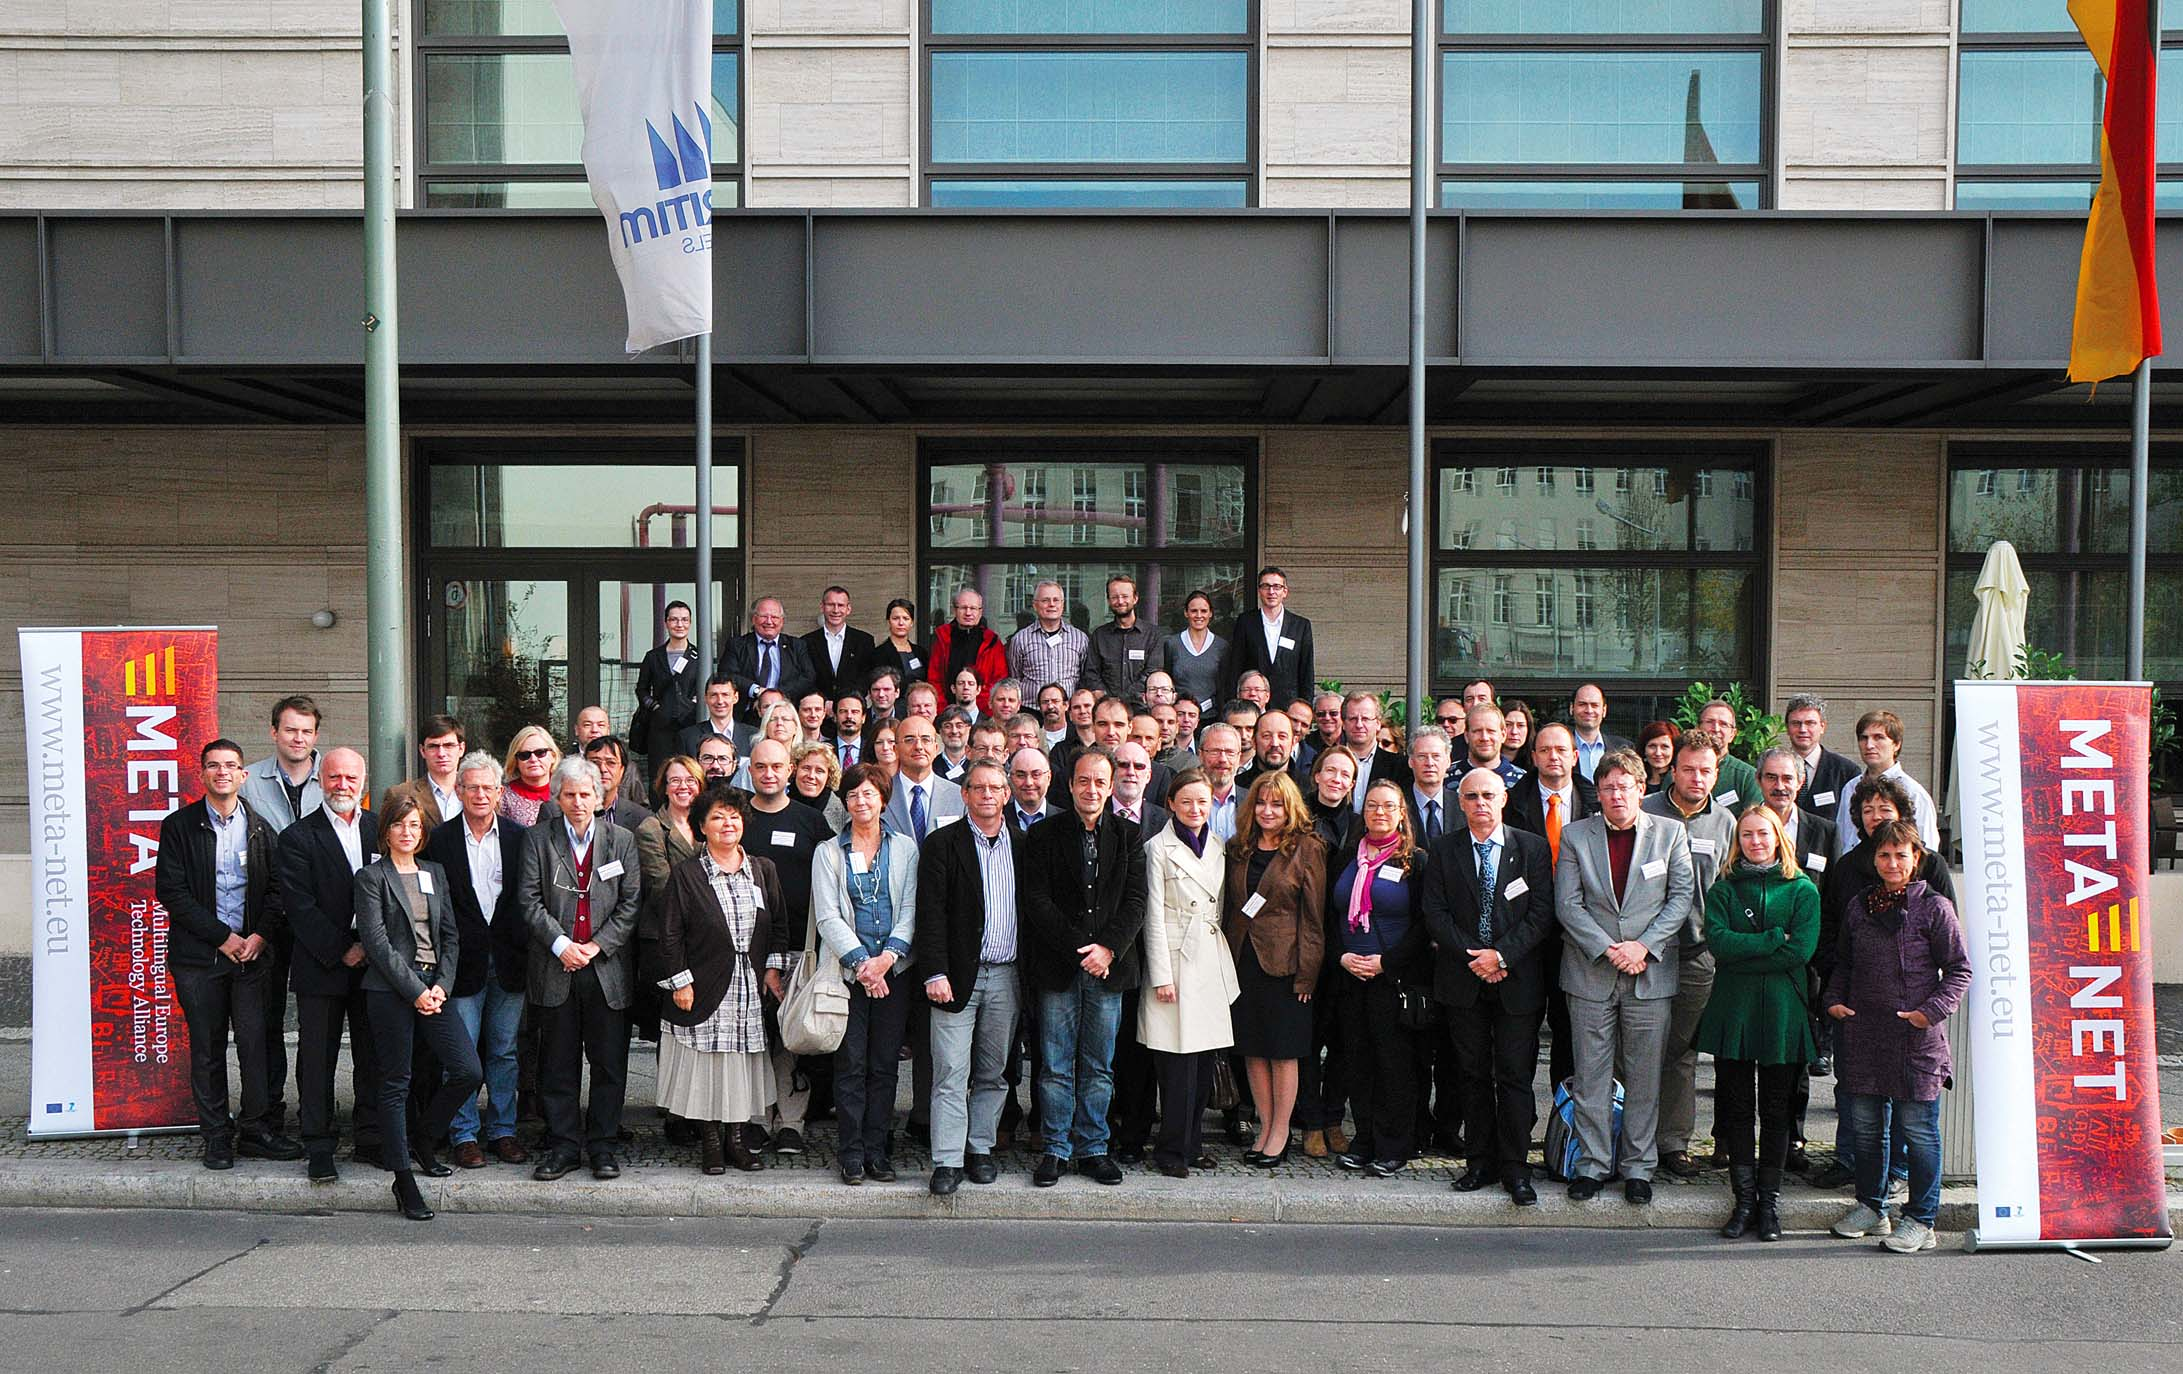
\includegraphics[width=\textwidth]{../_media/meta-net_team_ebook.jpg}
  }{%
    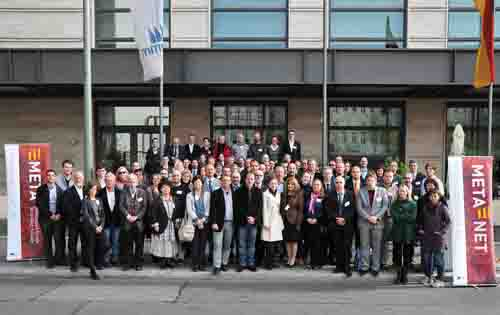
\includegraphics[width=\textwidth]{../_media/meta-net_team.jpg}
  }
    \caption{Oko 100 jezične tehnologije stručnjaci - Predstavnici zemalja i
      jezika zastupljenih u META-NET - raspravlja i finalizirani ključne
      rezultate i poruke Bijele knjige serije na sastanku u Berlinu, Njemačka,
      listopada 21/22, 2011.~--~\textcolor{grey1}{About 100 language technology
      experts -- representatives of the countries and languages represented in
      META-NET -- discussed and finalised the key results and messages of the
      White Paper Series at a meeting in Berlin, Germany, on October 21/22,
      2011.}}
    \medskip \colorrule{grey3}{\textwidth}{1.5pt}
\end{figure*} 

\cleardoublepage

\phantomsection\bsection[Niz Bijele Knjige META-NET -- The META-NET White Paper Series]{Niz bijele knjige META-NET --- The META-NET\ \ \ \ \ \ White Paper Series}
\label{whitepaperseries}

\vspace*{-5mm}
\centering
  \setlength{\tabcolsep}{2em}
  \begin{tabulary}{170mm}{LLL} \toprule
  baskijski & Basque & euskara \\
  bugarski & Bulgarian & български \\
  češki & Czech & čeština \\
  danski & Danish & dansk \\
  engleski & English & English \\
  estonski & Estonian & eesti \\
  finski & Finnish & suomi \\
  francuski & French & français \\
  galicijski & Galician & galego \\
  grčki & Greek & ελληνικά \\
  hrvatski & Croatian & hrvatski \\
  irski & Irish & Gaeilge \\
  islandski & Icelandic & íslenska \\
  katalonski & Catalan & català \\
  latvijski & Latvian & latviešu valoda \\
  litavski & Lithuanian & lietuvių kalba \\
  mađarski & Hungarian & magyar \\
  malteški & Maltese & Malti \\
  nizozemski & Dutch & Nederlands \\
  norveški bokmål & Norwegian Bokmål & bokmål \\
  norveški nýnorsk & Norwegian Nynorsk & nynorsk \\
  njemački & German & Deutsch \\  
  poljski & Polish & polski \\
  portugalski & Portuguese & português \\
  rumunjski & Romanian & română \\
  slovački & Slovak & slovenčina \\
  slovenski & Slovene & slovenščina \\
  srpski & Serbian & српски \\
  španjolski & Spanish & español \\
  švedski & Swedish & svenska \\
  talijanski & Italian & italiano \\ \bottomrule
\end{tabulary}

\end{document}
